%!TEX TS-program = xelatex
\documentclass[notes,12pt, aspectratio=169]{beamer}

\usepackage{amsmath,amsfonts,amssymb,amsthm,mathtools}  % пакеты для математики
%\usepackage{minted}

\usepackage[english, russian]{babel} % выбор языка для документа
\usepackage[utf8]{inputenc} % задание utf8 кодировки исходного tex файла
\usepackage[X2,T2A]{fontenc}        % кодировка

\usepackage{fontspec}         % пакет для подгрузки шрифтов
\setmainfont{Helvetica}  % задаёт основной шрифт документа

% why do we need \newfontfamily:
% http://tex.stackexchange.com/questions/91507/
\newfontfamily{\cyrillicfonttt}{Helvetica}
\newfontfamily{\cyrillicfont}{Helvetica}
\newfontfamily{\cyrillicfontsf}{Helvetica}

\usepackage{unicode-math}     % пакет для установки математического шрифта
% \setmathfont{Neo Euler} % шрифт для математики

\usepackage{polyglossia}      % Пакет, который позволяет подгружать русские буквы
\setdefaultlanguage{russian}  % Основной язык документа
\setotherlanguage{english}    % Второстепенный язык документа

% Шрифт для кода
\setmonofont[Scale=0.85]{Monaco}
\usepackage{verbments}

\usepackage{pgfpages}
% These slides also contain speaker notes. You can print just the slides,
% just the notes, or both, depending on the setting below. Comment out the want
% you want.
%\setbeameroption{hide notes} % Only slide
%\setbeameroption{show only notes} % Only notes
%\setbeameroption{show notes on second screen=right} % Both

\usepackage{array}

\usepackage{tikz}
\usepackage{verbatim}
\setbeamertemplate{note page}{\pagecolor{yellow!5}\insertnote}
\usetikzlibrary{positioning}
\usetikzlibrary{snakes}
\usetikzlibrary{calc}
\usetikzlibrary{arrows}
\usetikzlibrary{decorations.markings}
\usetikzlibrary{shapes.misc}
\usetikzlibrary{matrix,shapes,arrows,fit,tikzmark}

\usepackage{hyperref}
\usepackage{lipsum}
\usepackage{multimedia}
\usepackage{multirow}
\usepackage{dcolumn}
\usepackage{bbm}
\newcolumntype{d}[0]{D{.}{.}{5}}

\usepackage{changepage}
\usepackage{appendixnumberbeamer}
\newcommand{\beginbackup}{
   \newcounter{framenumbervorappendix}
   \setcounter{framenumbervorappendix}{\value{framenumber}}
   \setbeamertemplate{footline}
   {
     \leavevmode%
     \hline
     box{%
       \begin{beamercolorbox}[wd=\paperwidth,ht=2.25ex,dp=1ex,right]{footlinecolor}%
%         \insertframenumber  \hspace*{2ex} 
       \end{beamercolorbox}}%
     \vskip0pt%
   }
 }
\newcommand{\backupend}{
   \addtocounter{framenumbervorappendix}{-\value{framenumber}}
   \addtocounter{framenumber}{\value{framenumbervorappendix}} 
}

% для имитации питоновского синтаксиса 
\newcommand{\pgr}[1]{{\color{green} \textbf{#1}}}


%%%%%%%%%% Работа с картинками %%%%%%%%%
\usepackage{graphicx}                  % Для вставки рисунков
\usepackage{graphics}
\graphicspath{{images/}}    % можно указать папки с картинками
\usepackage{wrapfig}                   % Обтекание рисунков и таблиц текстом

\usepackage[space]{grffile}
\usepackage{booktabs}

% These are my colors -- there are many like them, but these ones are mine.
\definecolor{blue}{RGB}{0,114,178}
\definecolor{red}{RGB}{213,94,0}
\definecolor{yellow}{RGB}{240,228,66}
\definecolor{green}{RGB}{0,128, 0}

\hypersetup{
  colorlinks=false,
  linkbordercolor = {white},
  linkcolor = {blue}
}


%% I use a beige off white for my background
\definecolor{MyBackground}{RGB}{255,253,218}

%% Uncomment this if you want to change the background color to something else
%\setbeamercolor{background canvas}{bg=MyBackground}

%% Change the bg color to adjust your transition slide background color!
\newenvironment{transitionframe}{
  \setbeamercolor{background canvas}{bg=yellow}
  \begin{frame}}{
    \end{frame}
}

\setbeamercolor{frametitle}{fg=blue}
\setbeamercolor{title}{fg=black}
\setbeamertemplate{footline}[frame number]
\setbeamertemplate{navigation symbols}{} 
\setbeamertemplate{itemize items}{-}
\setbeamercolor{itemize item}{fg=blue}
\setbeamercolor{itemize subitem}{fg=blue}
\setbeamercolor{enumerate item}{fg=blue}
\setbeamercolor{enumerate subitem}{fg=blue}
\setbeamercolor{button}{bg=MyBackground,fg=blue,}


% If you like road maps, rather than having clutter at the top, have a roadmap show up at the end of each section 
% (and after your introduction)
% Uncomment this is if you want the roadmap!
% \AtBeginSection[]
% {
%    \begin{frame}
%        \frametitle{Roadmap of Talk}
%        \tableofcontents[currentsection]
%    \end{frame}
% }
\setbeamercolor{section in toc}{fg=blue}
\setbeamercolor{subsection in toc}{fg=red}
\setbeamersize{text margin left=1em,text margin right=1em} 

% списки, которые растягиваются на всю величину слайда 
\newenvironment{wideitemize}{\itemize\addtolength{\itemsep}{10pt}}{\enditemize}

\newcommand{\ENC}{\text{ENC}}
\newcommand{\DEC}{\text{DEC}}


\title[]{\textcolor{blue}{Глубокое обучение и вообще}}
\author{Ульянкин Филипп}
\date{\today}

\begin{document}

%%% TIKZ STUFF
\tikzset{   
        every picture/.style={remember picture,baseline},
        every node/.style={anchor=base,align=center,outer sep=1.5pt},
        every path/.style={thick},
        }
\newcommand\marktopleft[1]{%
    \tikz[overlay,remember picture] 
        \node (marker-#1-a) at (-.3em,.3em) {};%
}
\newcommand\markbottomright[2]{%
    \tikz[overlay,remember picture] 
        \node (marker-#1-b) at (0em,0em) {};%
}
\tikzstyle{every picture}+=[remember picture] 
\tikzstyle{mybox} =[draw=black, very thick, rectangle, inner sep=10pt, inner ysep=20pt]
\tikzstyle{fancytitle} =[draw=black,fill=red, text=white]
%%%% END TIKZ STUFF

% Title Slide
\begin{frame}
\maketitle
\centering \textbf{\color{blue} Посиделка 12:}  Seq2Seq и Attention
\end{frame}

\begin{frame}{Agenda}
\begin{wideitemize}
	\item  Мультимодальные модели
	\item  История автоперевода
	\item  Нейросетевой автоперевод
	\item  Механизмы внимания
\end{wideitemize} 
\end{frame}


\begin{transitionframe}
	\begin{center}
		\Huge  Мультимодальные модели
	\end{center}
\end{transitionframe}


\begin{frame}{Word2vec: семантическое пространство}
	\begin{center}
		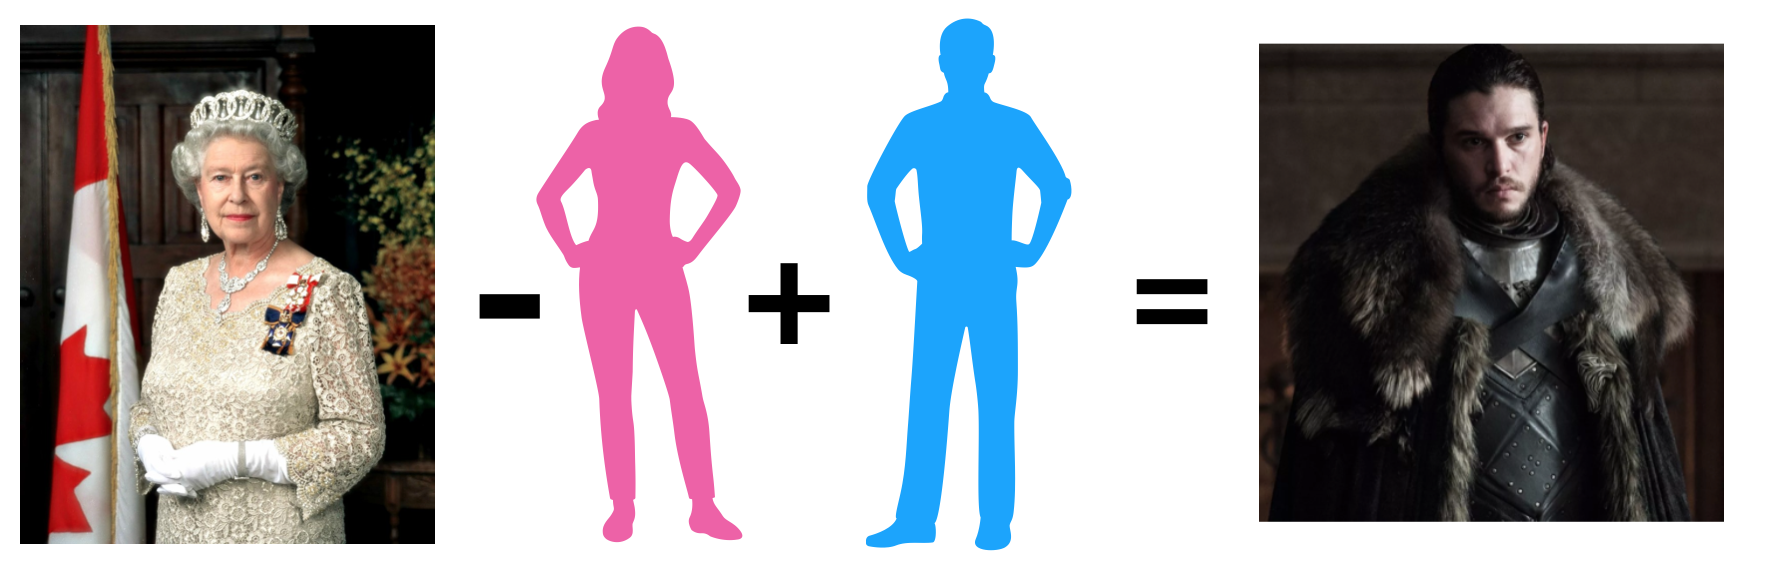
\includegraphics[width=.7\linewidth]{w2v_arith.png}
	\end{center}

	\begin{center}
	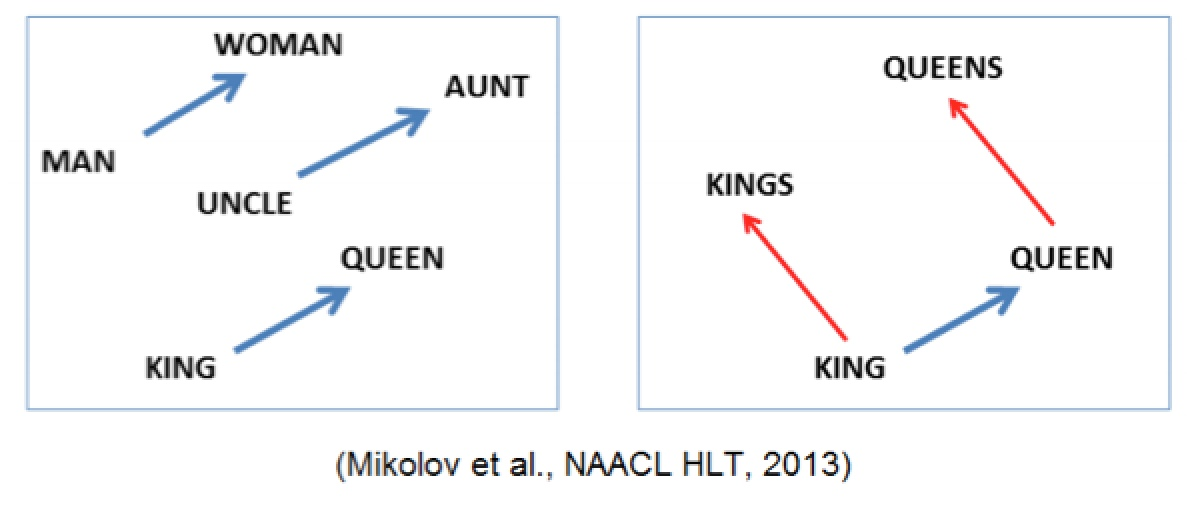
\includegraphics[width=.6\linewidth]{w2v_king1.jpg}
\end{center}
\end{frame} 


\begin{frame}{Векторные пространства}
		\begin{wideitemize} 
			\item  Мы умеем обучать векторные пространства для какого-то одного типа объектов
			\item  \alert{Вот бы можно было учить векторные пространства сразу для разных объектов} 
		\end{wideitemize} 
\end{frame} 


\begin{frame}{Мультимодальное векторное пространство (2014)}
	\begin{center}
		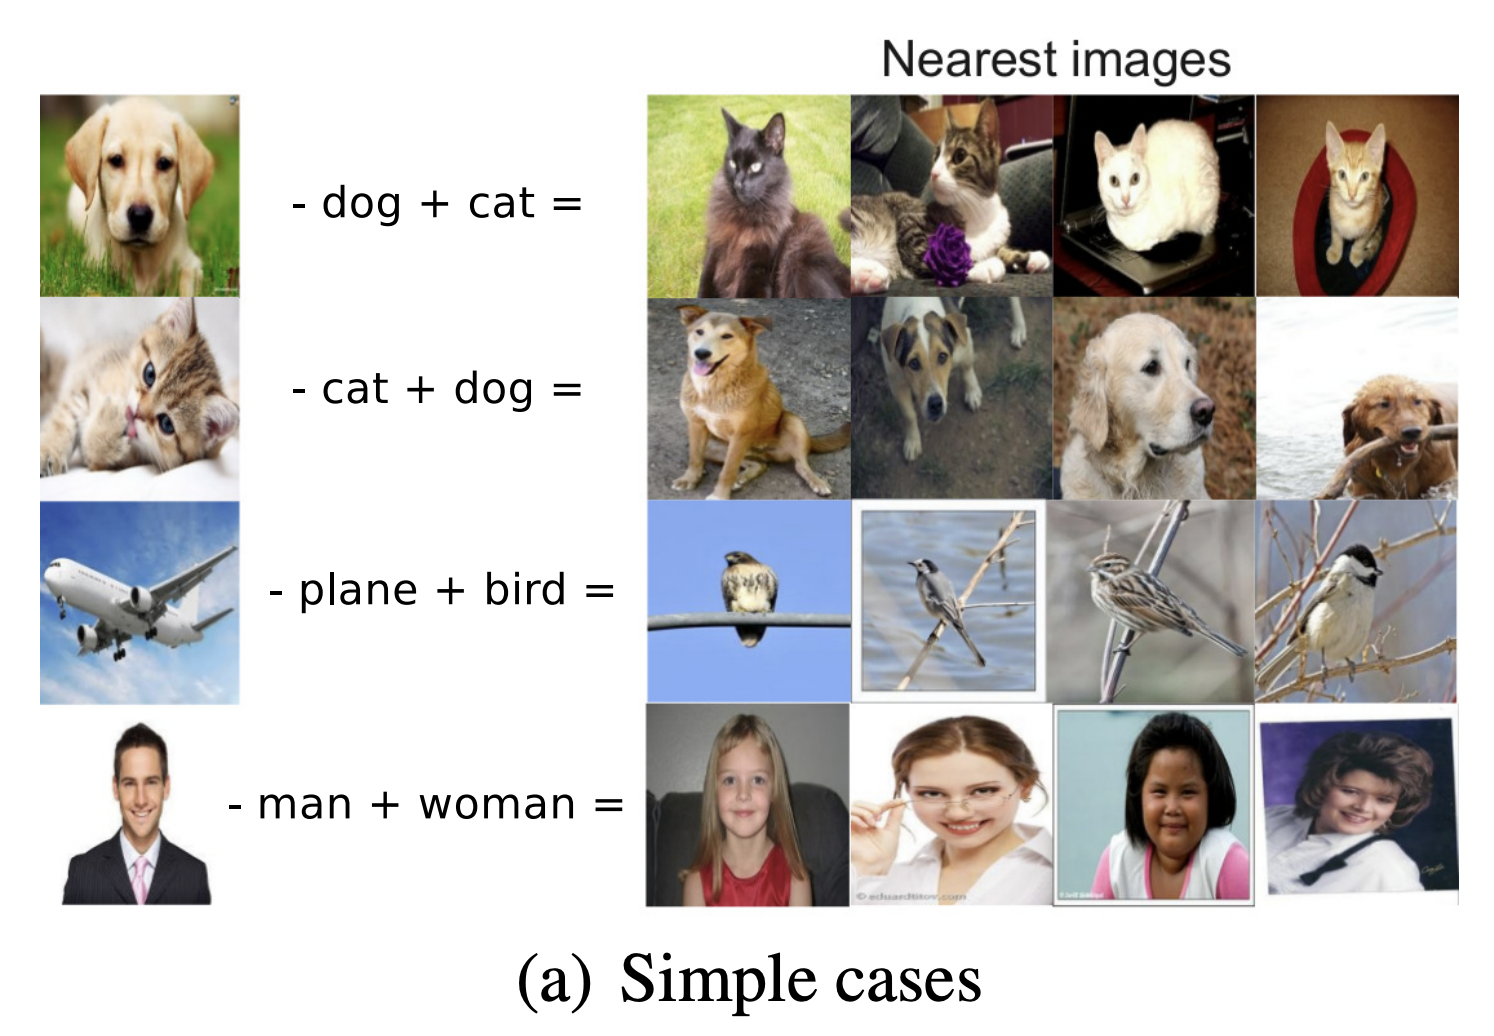
\includegraphics[width=.68\linewidth]{im_and_wd0.png}
	\end{center}
	\vfill
\footnotesize  {\color{blue} \url{https://arxiv.org/pdf/1411.2539.pdf}}
\end{frame} 


\begin{frame}{Мультимодальное векторное пространство (2014)}
	\begin{center}
		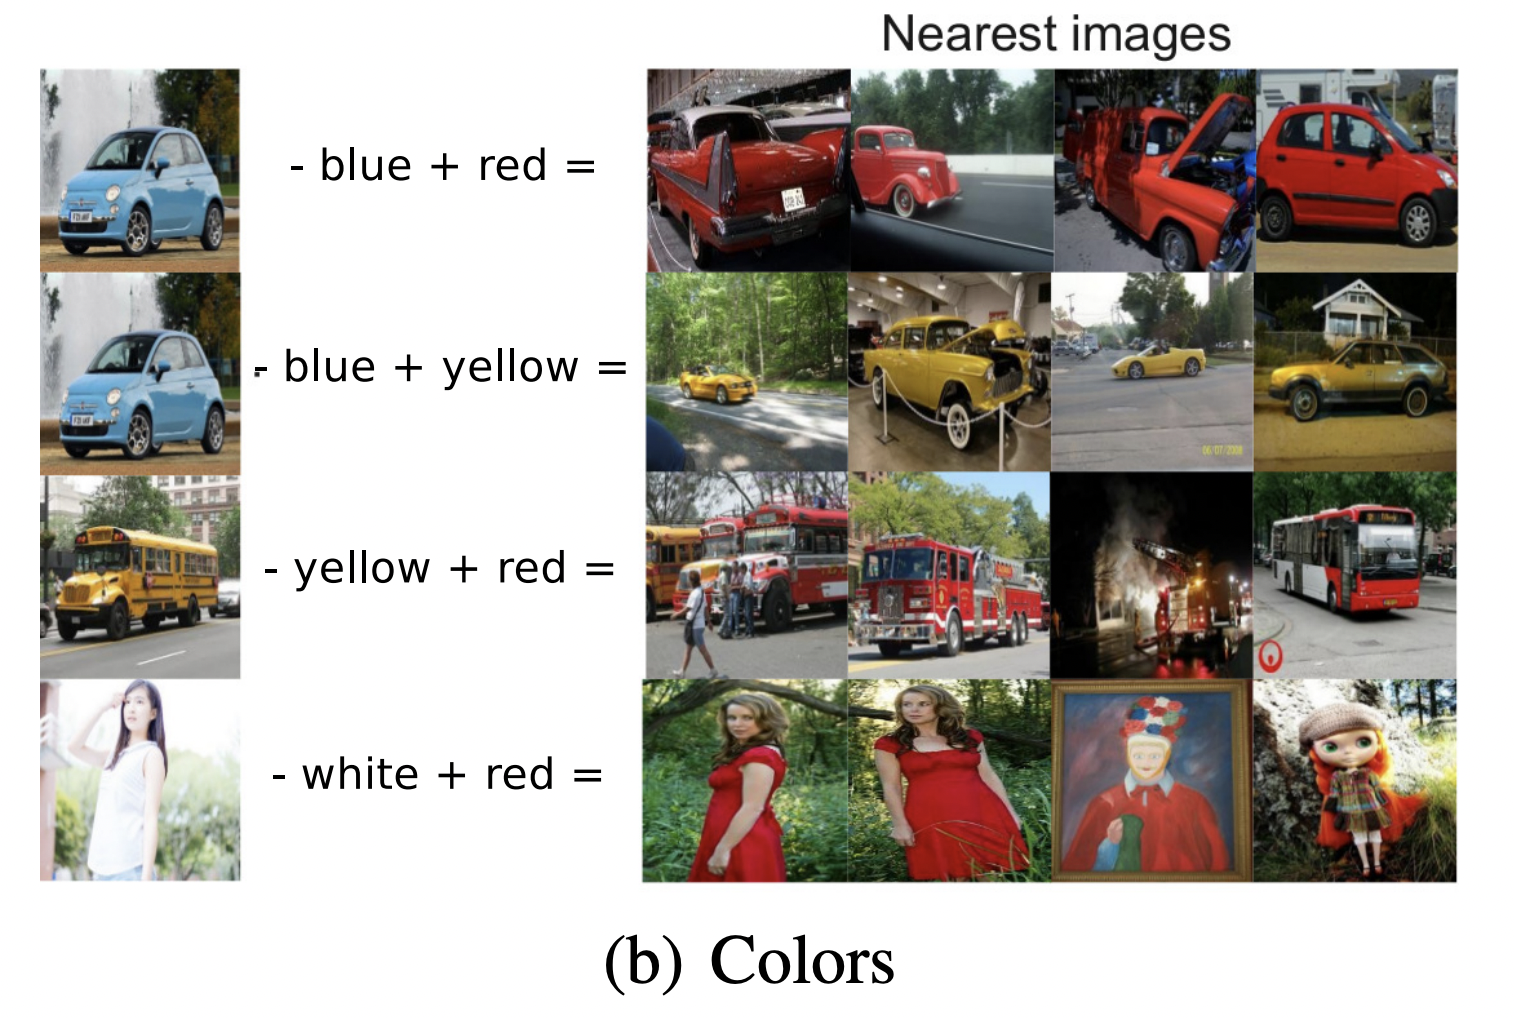
\includegraphics[width=.7\linewidth]{im_and_wd2.png}
	\end{center}
	\vfill
	\footnotesize  {\color{blue} \url{https://arxiv.org/pdf/1411.2539.pdf}}
\end{frame} 


\begin{frame}{Мультимодальное векторное пространство (2014)}
	\begin{center}
		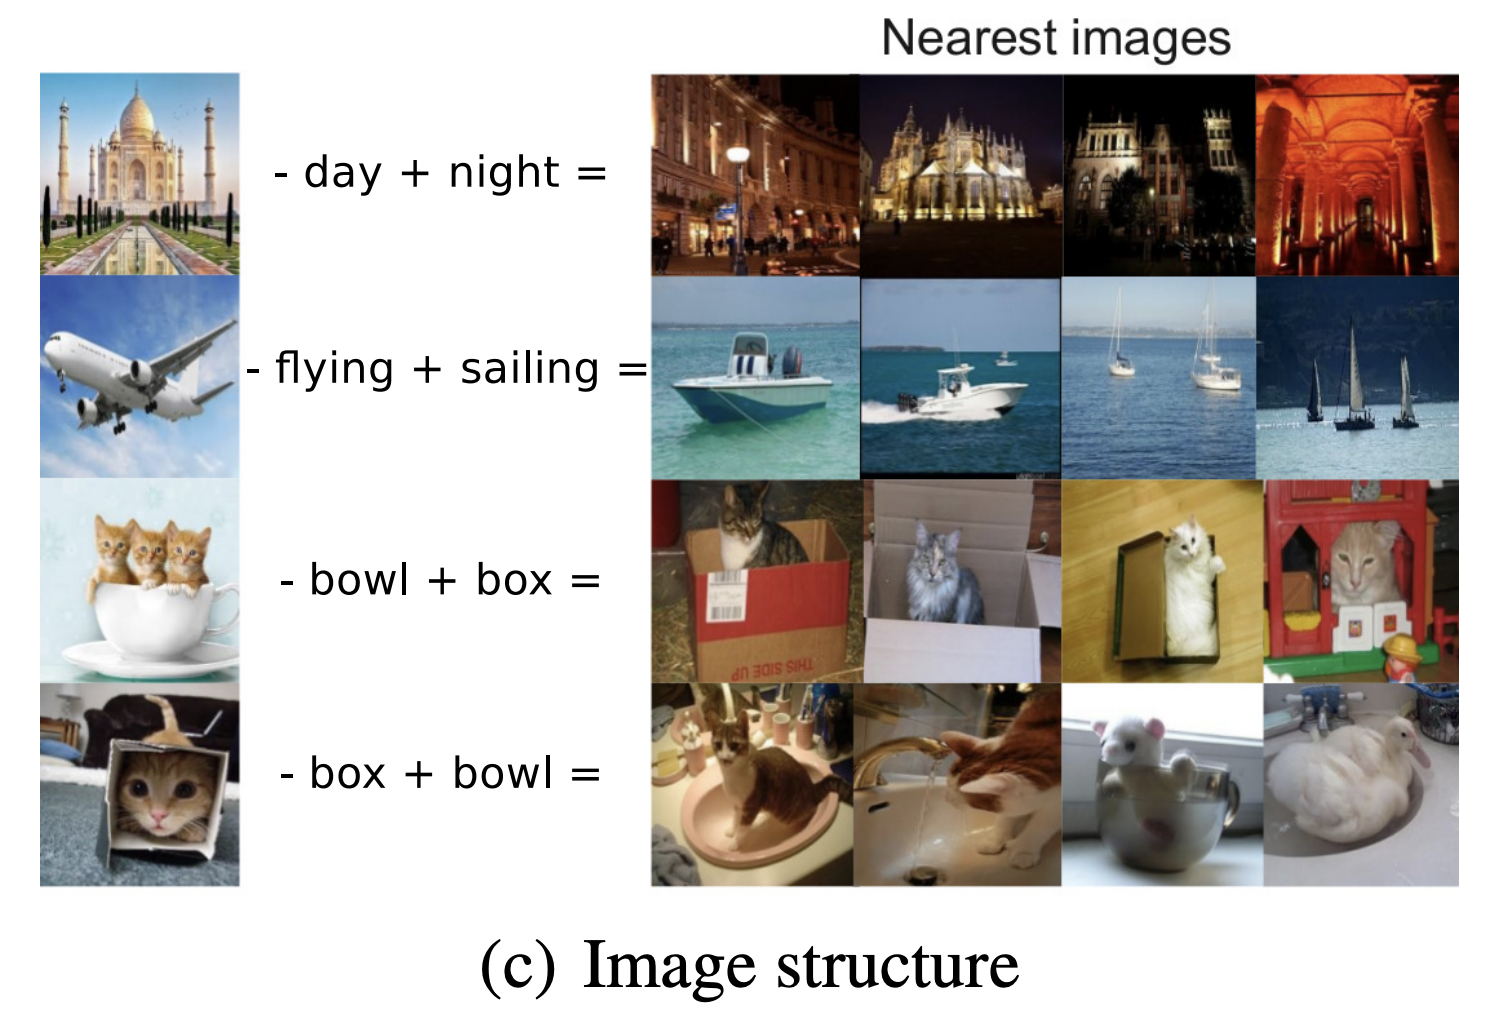
\includegraphics[width=.7\linewidth]{im_and_wd1.png}
	\end{center}
	\vfill
	\footnotesize  {\color{blue} \url{https://arxiv.org/pdf/1411.2539.pdf}}
\end{frame} 


\begin{frame}{Мультимодальное векторное пространство (2014)}
	\begin{center}
		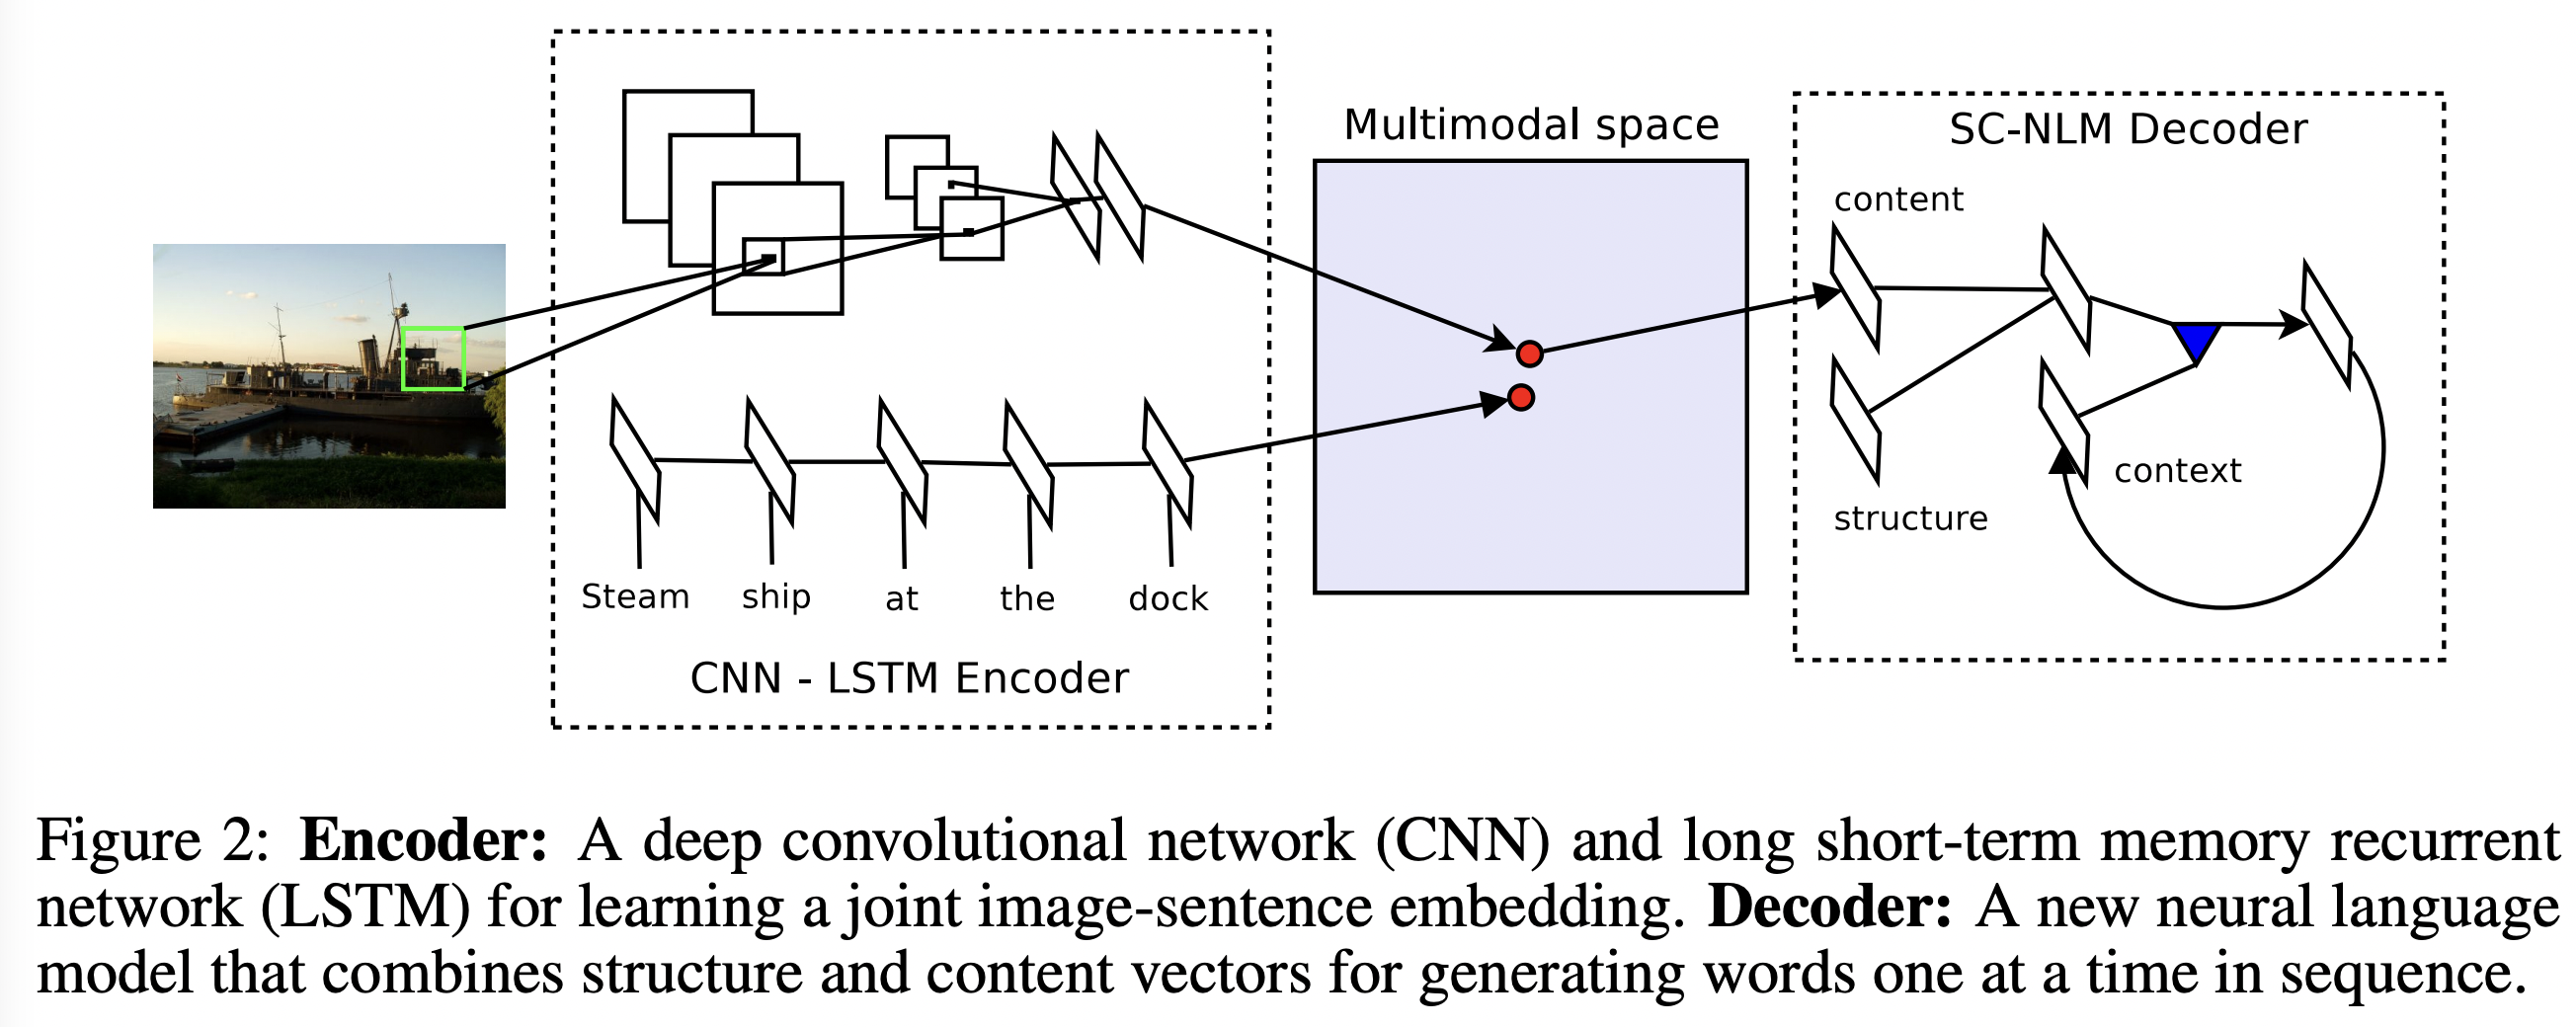
\includegraphics[width=.85\linewidth]{text_img_space.png}
	\end{center}
	\vfill
	\footnotesize  {\color{blue} \url{https://arxiv.org/pdf/1411.2539.pdf}}
\end{frame} 


\begin{frame}{Генерация текста по картинке (2015)}
	\begin{center}
		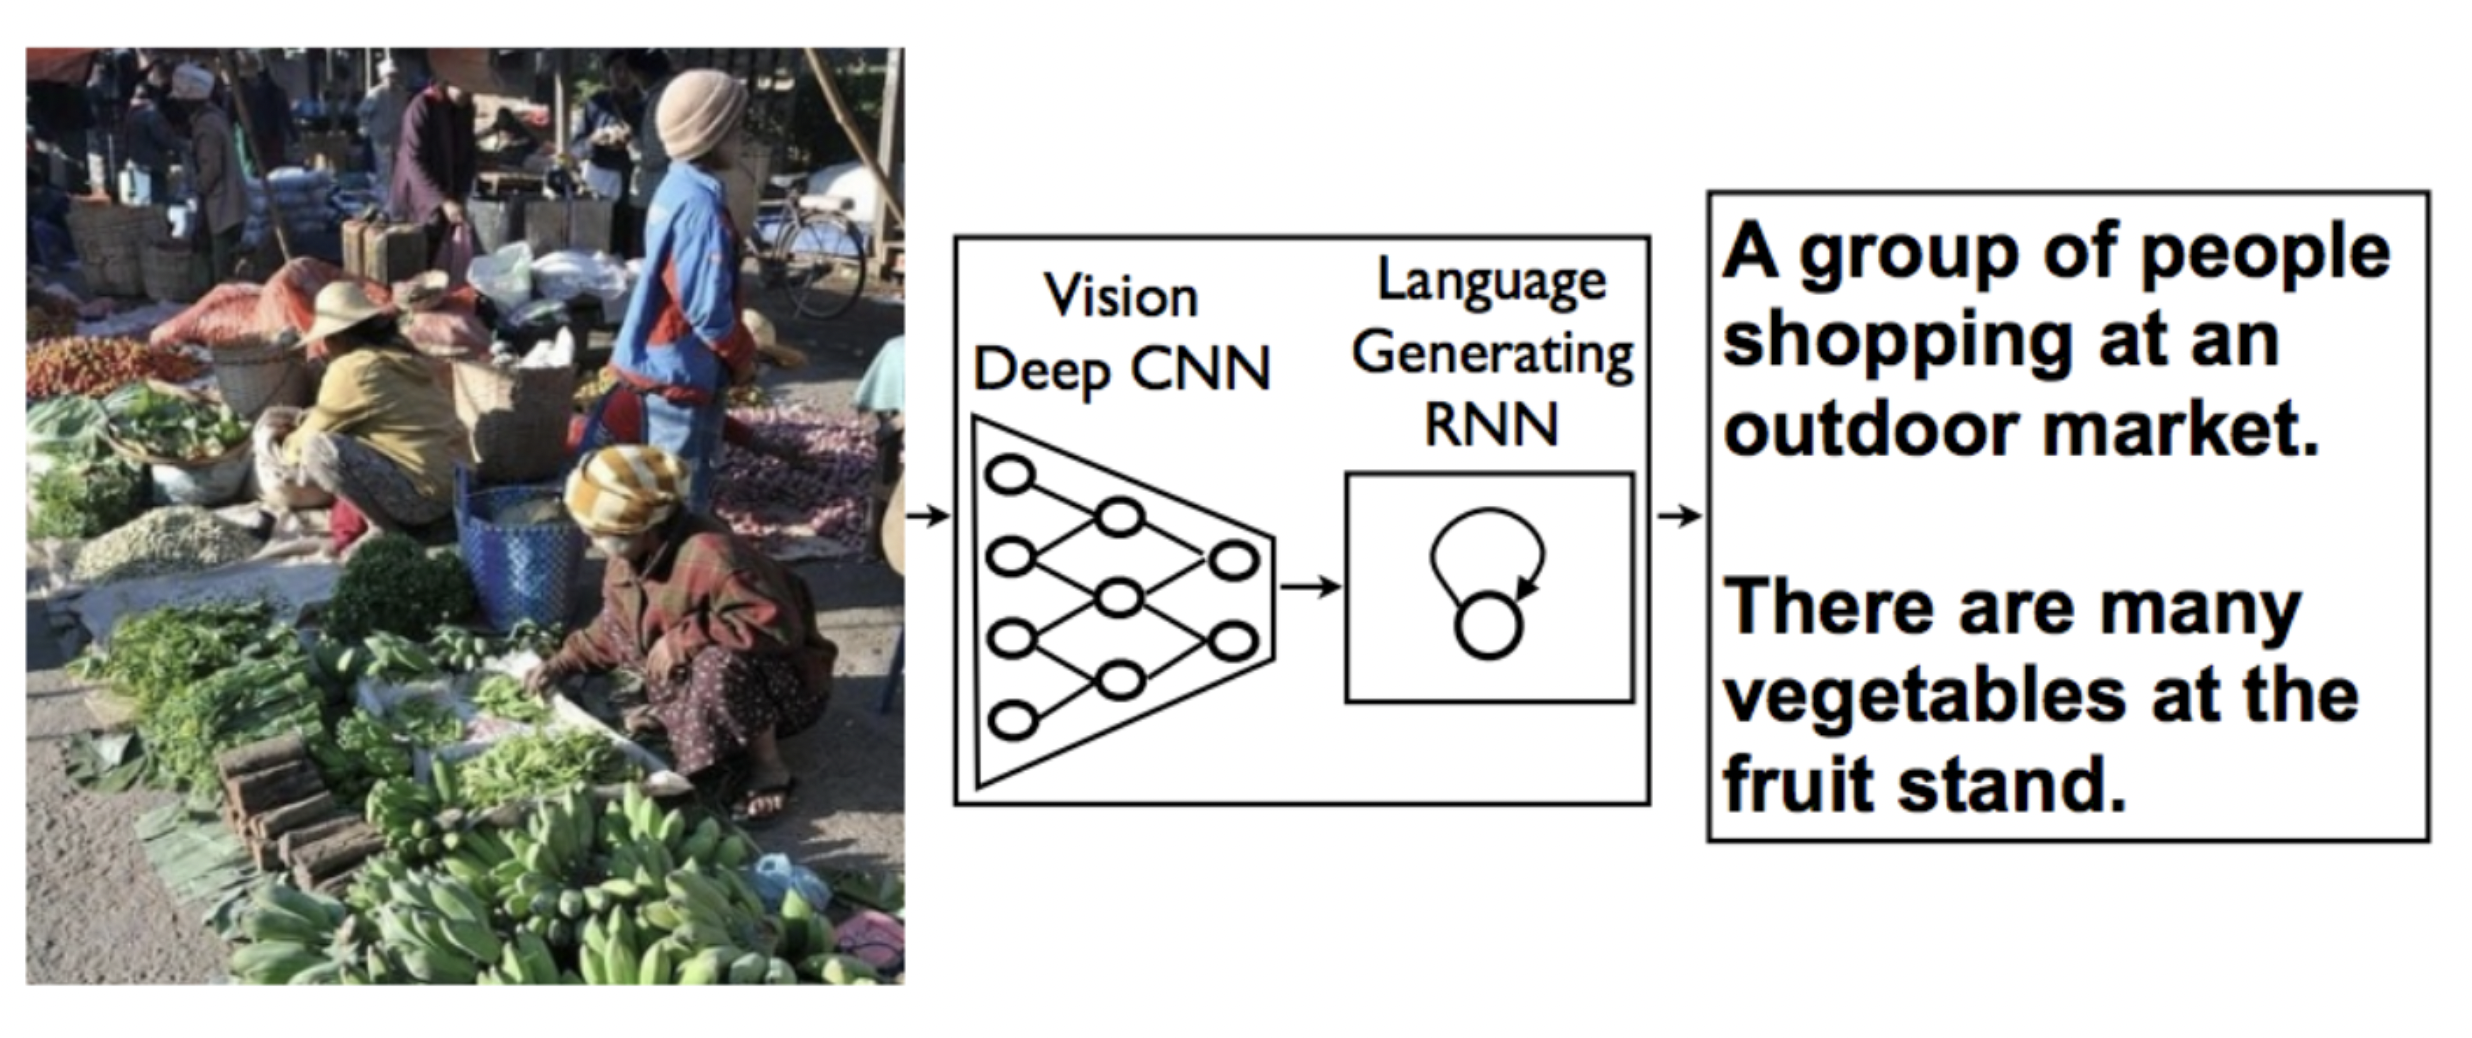
\includegraphics[width=.7\linewidth]{text_by_pic.png}
	\end{center}
	\vfill
	\footnotesize  {\color{blue} \url{https://arxiv.org/pdf/1411.4555.pdf}}
\end{frame} 


\begin{frame}{Генерация текста по картинке (2015)}
	\begin{center}
		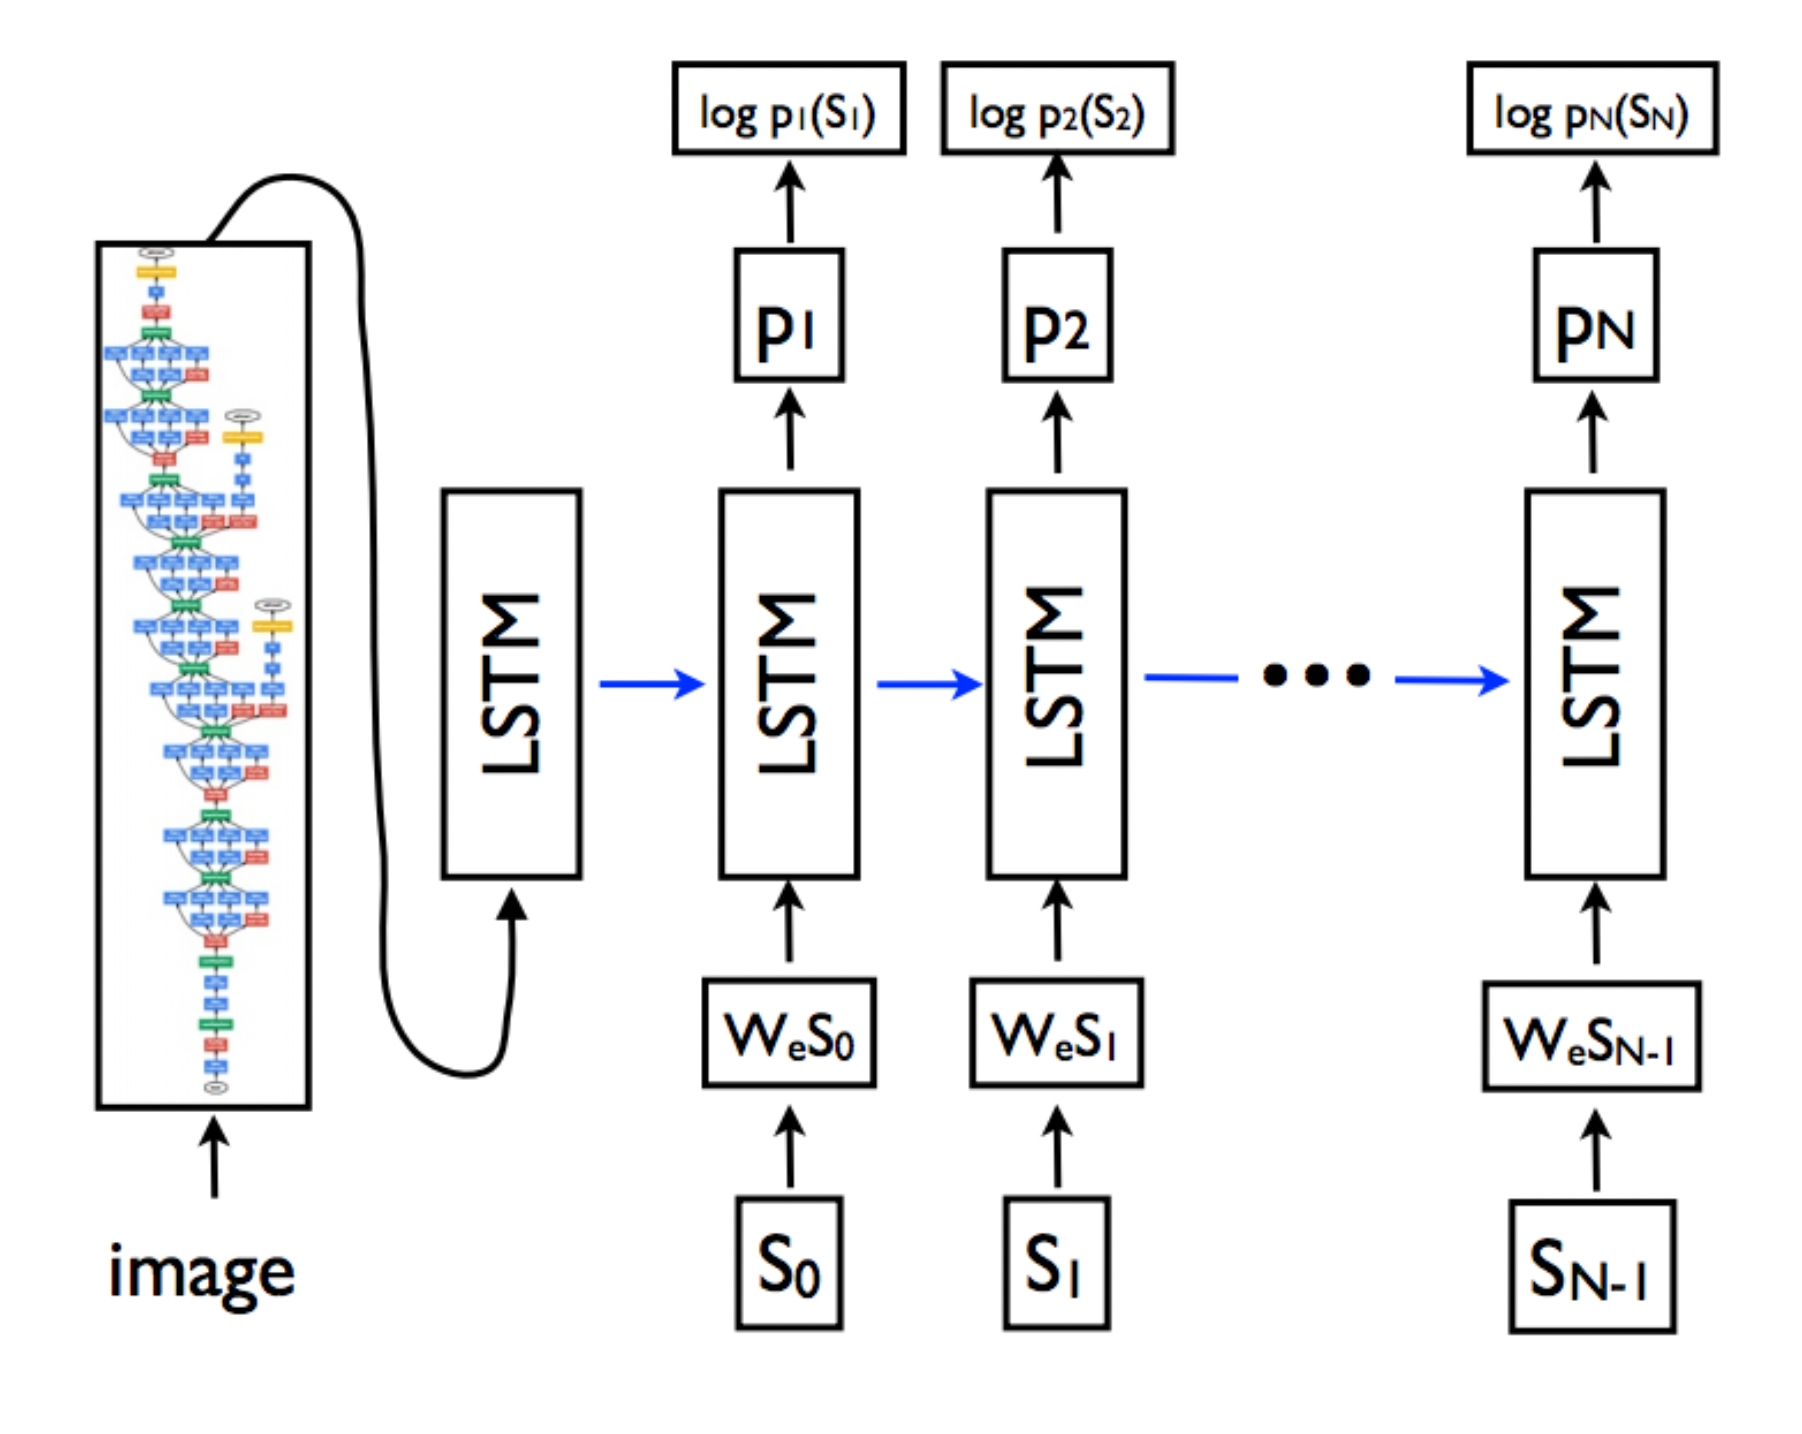
\includegraphics[width=.5\linewidth]{text_by_pic_model.png}
	\end{center}
	\vfill
	\footnotesize  {\color{blue} \url{https://arxiv.org/pdf/1411.4555.pdf}}
\end{frame} 


\begin{frame}{Генерация текста по картинке (2015)}
	\begin{center}
		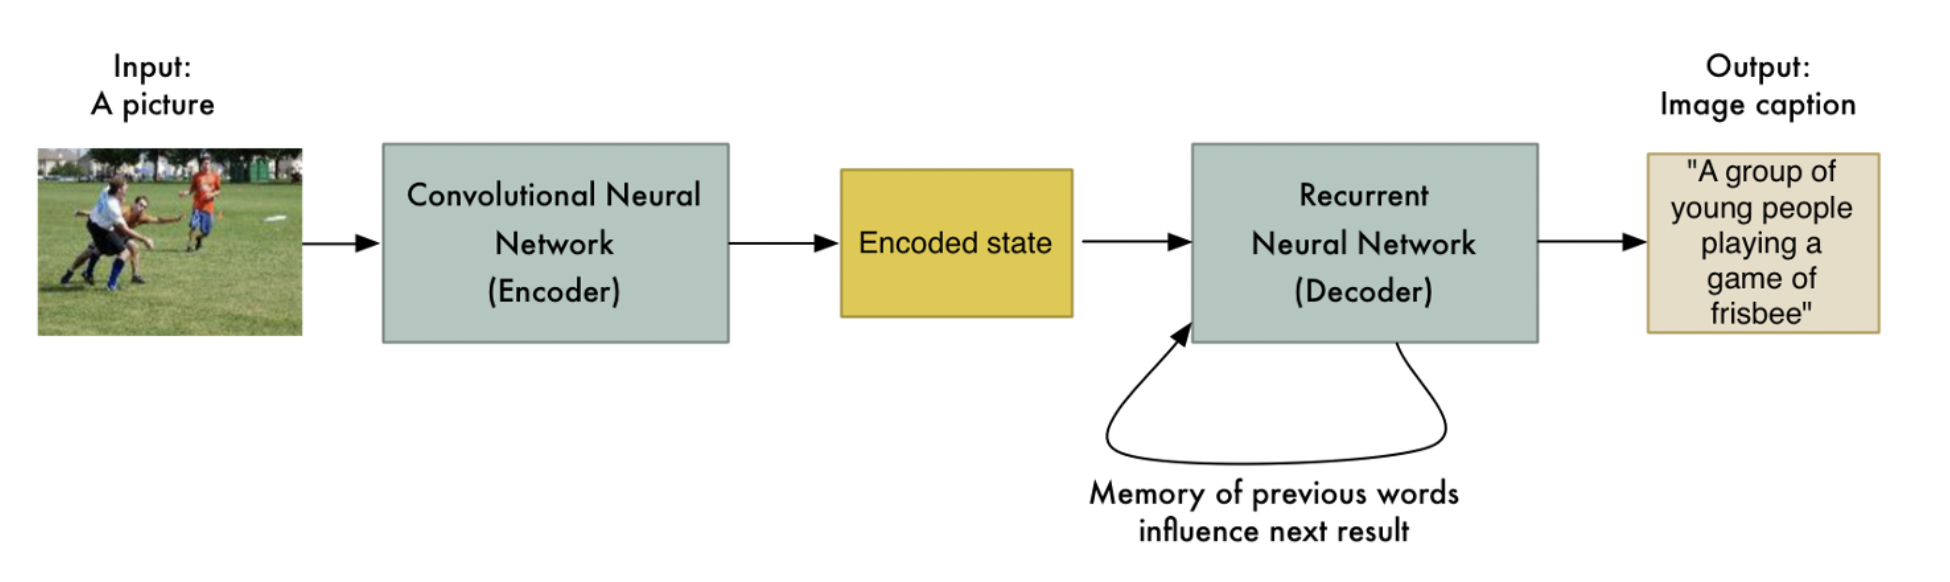
\includegraphics[width=.95\linewidth]{pic_text_model2.png}
	\end{center}
	\vfill
	\footnotesize  {\color{blue} \url{https://arxiv.org/pdf/1411.4555.pdf}}
\end{frame} 


\begin{frame}{Генерация текста по картинке (2015)}
	\begin{center}
		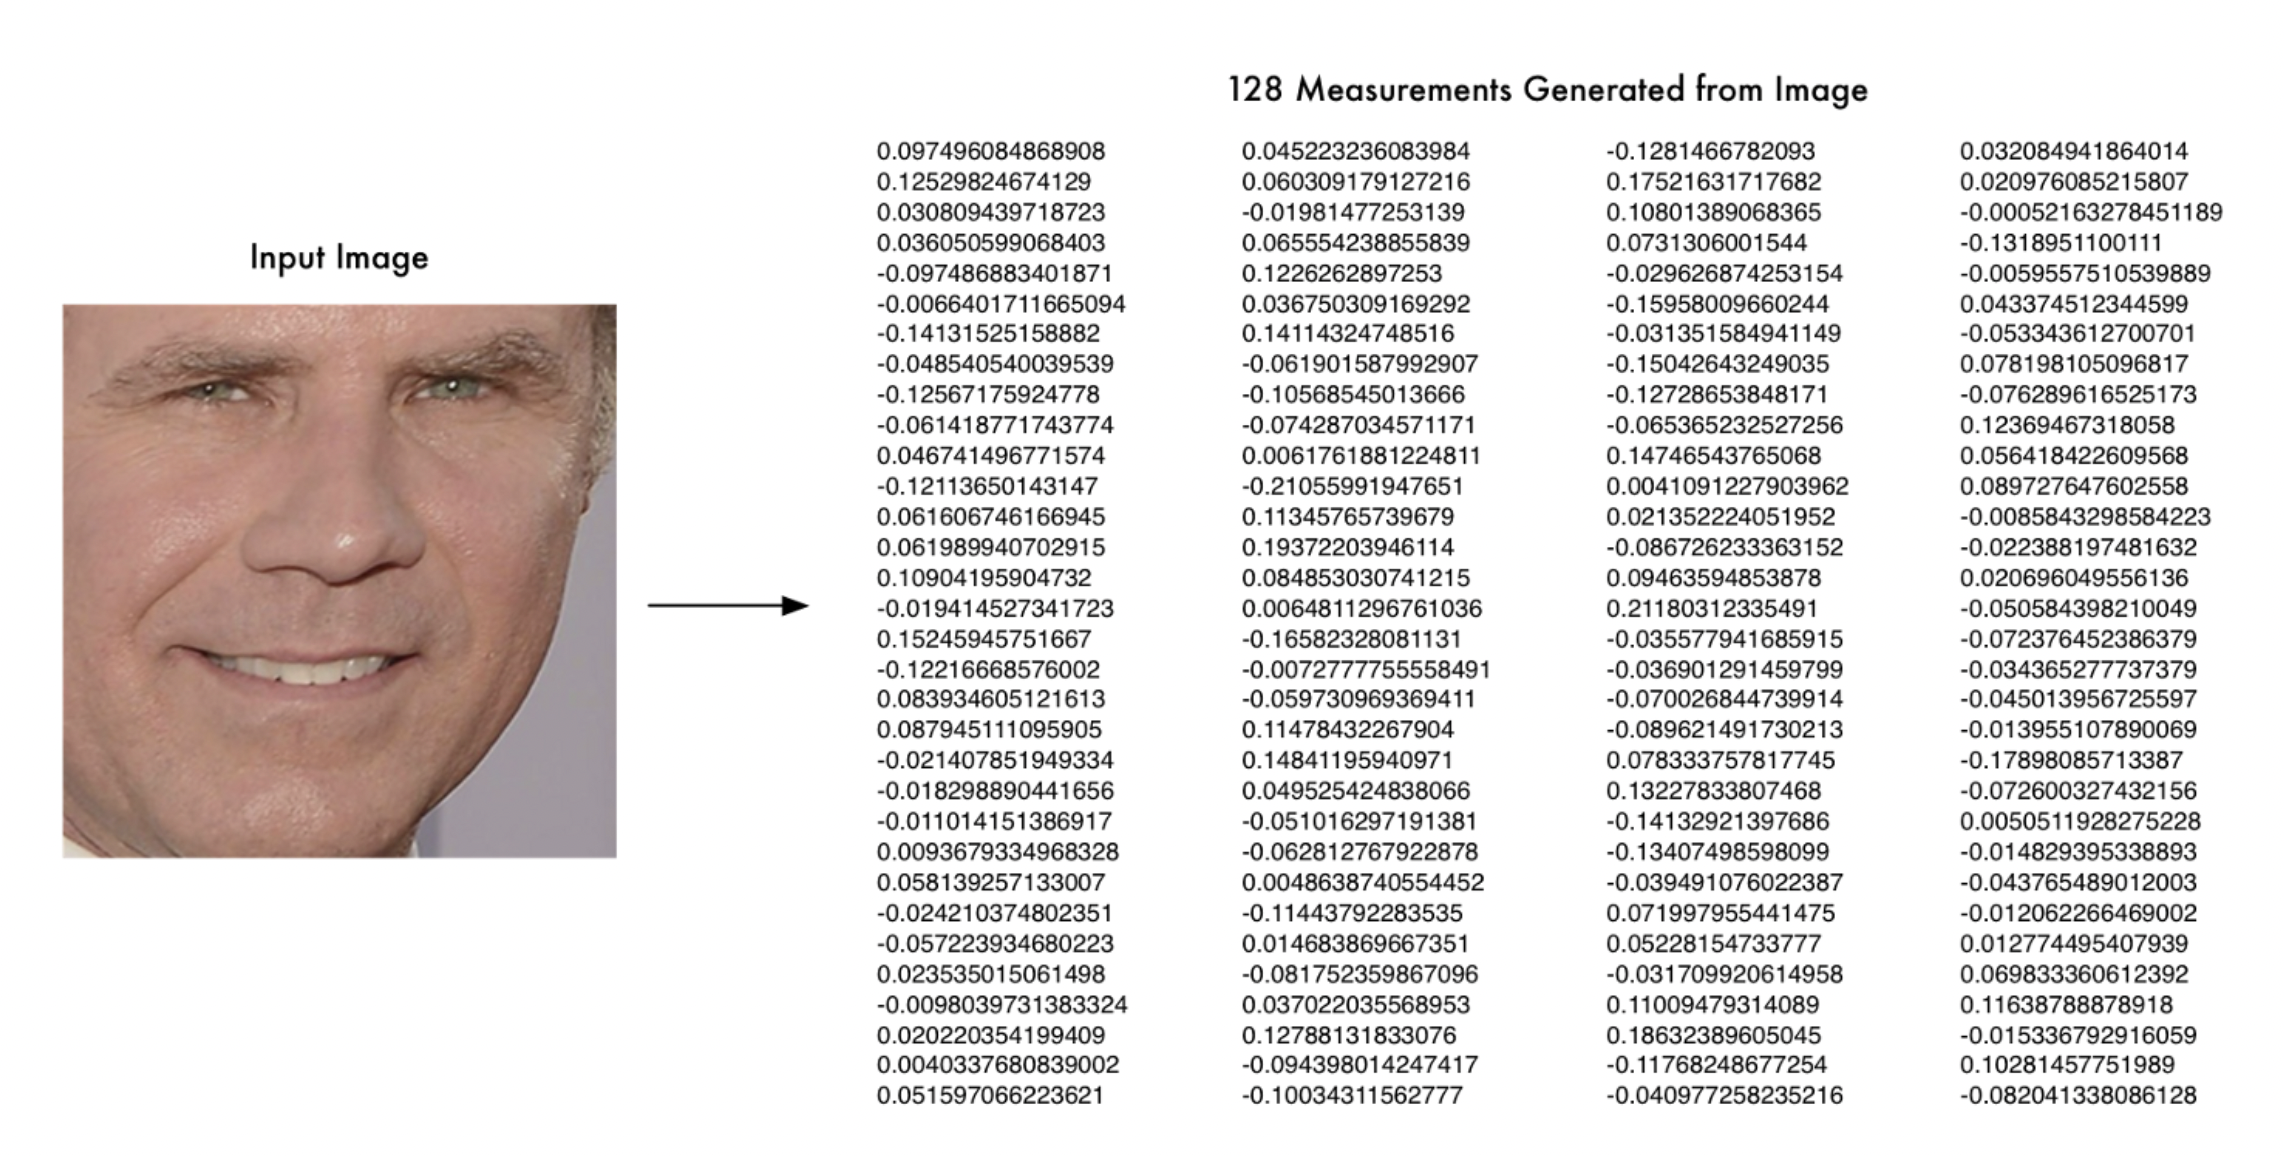
\includegraphics[width=.8\linewidth]{pic_text_face.png}
	\end{center}
	\vfill
	\footnotesize  {\color{blue} \url{https://arxiv.org/pdf/1411.4555.pdf}}
\end{frame} 



\begin{frame}{Генерация текста по картинке (2015)}
	\begin{center}
		\includegraphics[width=.65\linewidth]{text_by_pic_ex.png}
	\end{center}
	\vfill
	\footnotesize  {\color{blue} \url{https://arxiv.org/pdf/1411.4555.pdf}}
\end{frame} 


\begin{frame}{Генерация текста по картинке (2015)}
	\begin{center}
		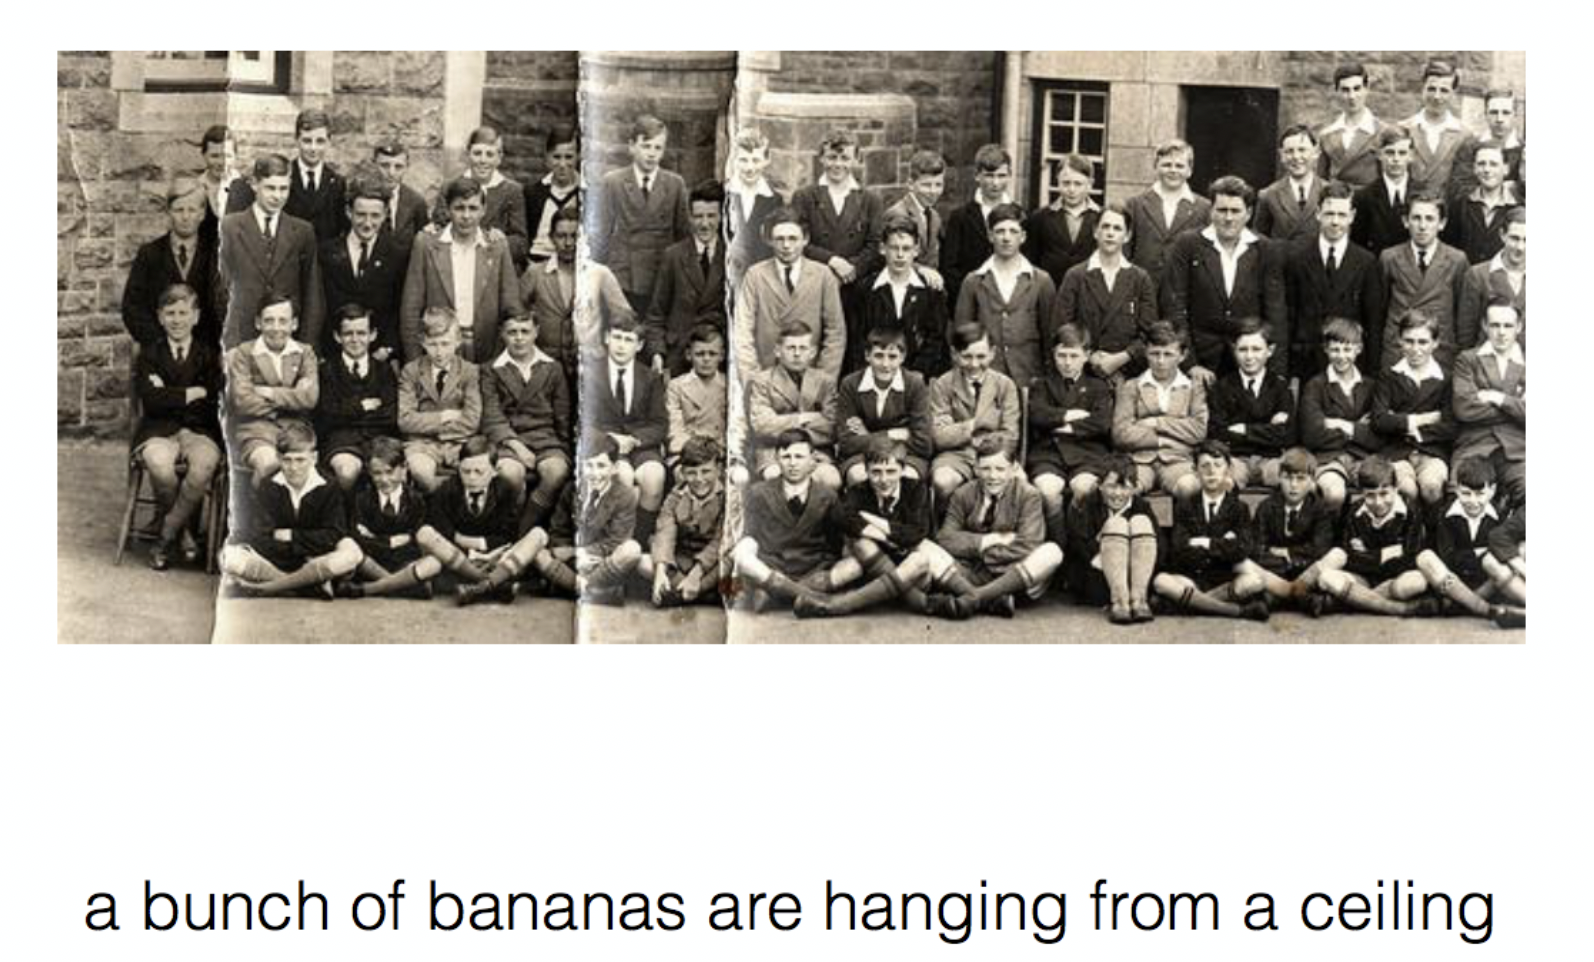
\includegraphics[width=.7\linewidth]{text_by_pic_ex2.png}
	\end{center}
	\vfill
	\footnotesize  {\color{blue} \url{https://arxiv.org/pdf/1411.4555.pdf}}
\end{frame} 


\begin{frame}{Генерация картинок по тексту (2022)}
	\begin{center}
		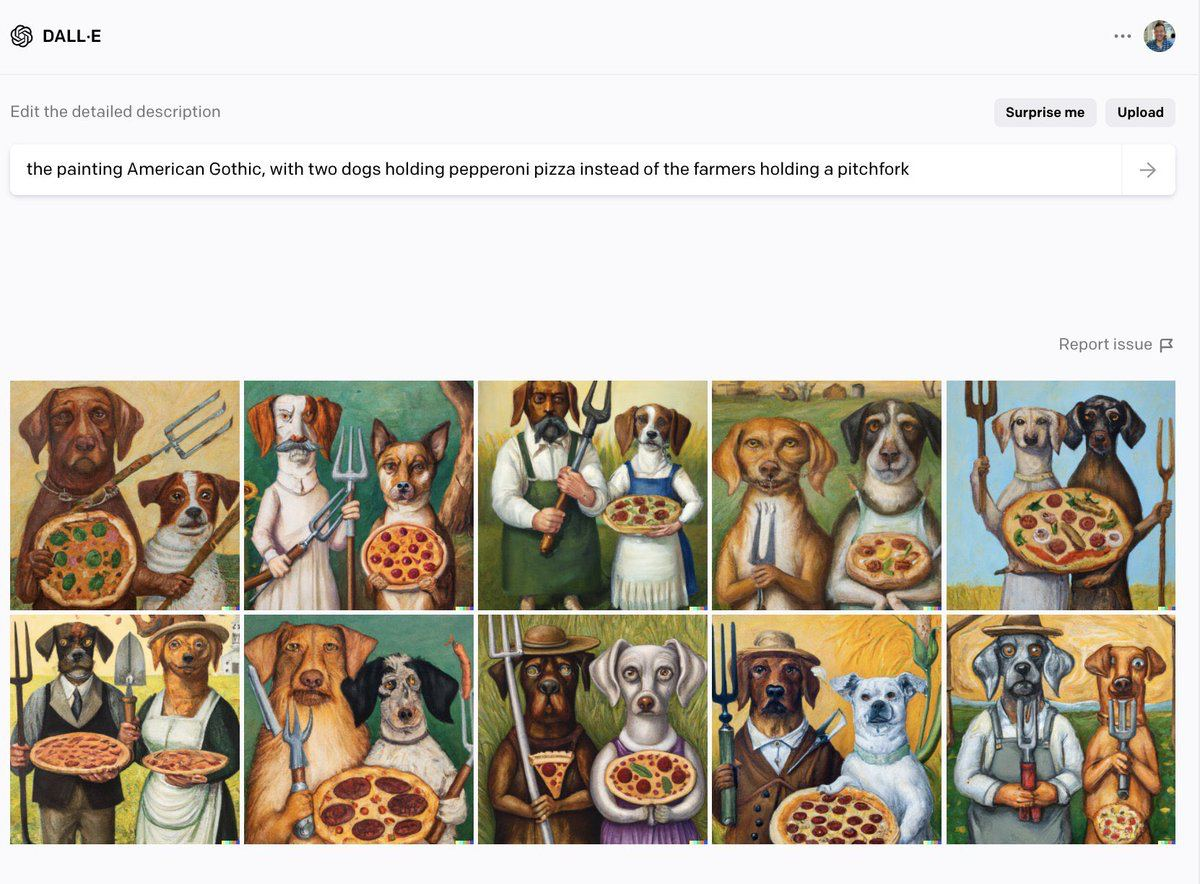
\includegraphics[width=.6\linewidth]{dogs_dalle.png}
	\end{center}
	\vfill
	\footnotesize  {\color{blue} \url{https://openai.com/dall-e-2/} \\ \url{https://arxiv.org/pdf/2204.06125.pdf}} 
\end{frame} 



\begin{frame}{Генерация картинок по тексту (2022)}
	\begin{center}
		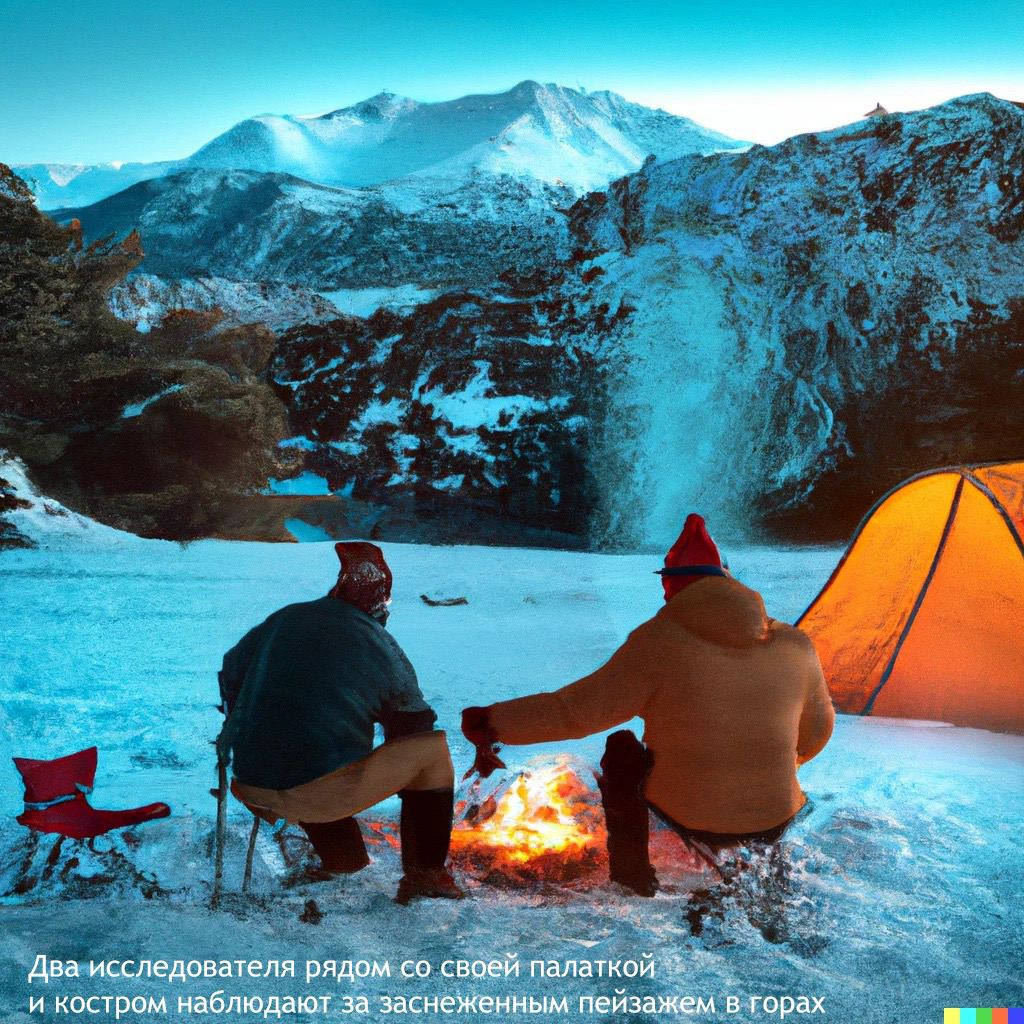
\includegraphics[width=.45\linewidth]{dalle_ex2.png}
	\end{center}
	\vfill
\footnotesize  {\color{blue} \url{https://openai.com/dall-e-2/} \\ \url{https://arxiv.org/pdf/2204.06125.pdf}} 
\end{frame} 



\begin{frame}{Генерация картинок по тексту (2022)}
	\begin{center}
		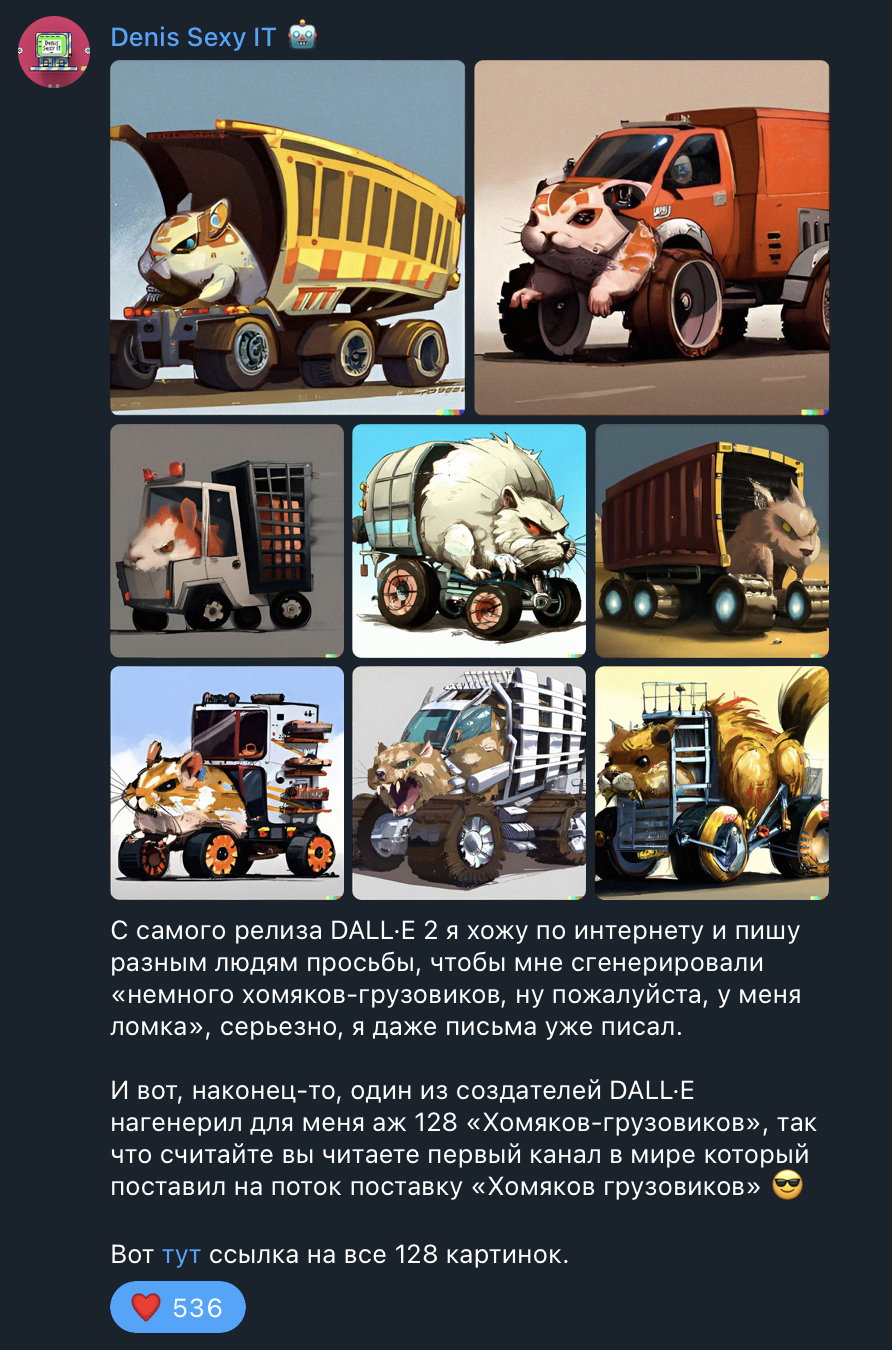
\includegraphics[width=.3\linewidth]{humsters.png}
	\end{center}
	\vfill
	\footnotesize  {\color{blue} \url{https://t.me/denissexy}} 
\end{frame} 



\begin{frame}{Генерация картинок по тексту (2022)}
	\begin{center}
		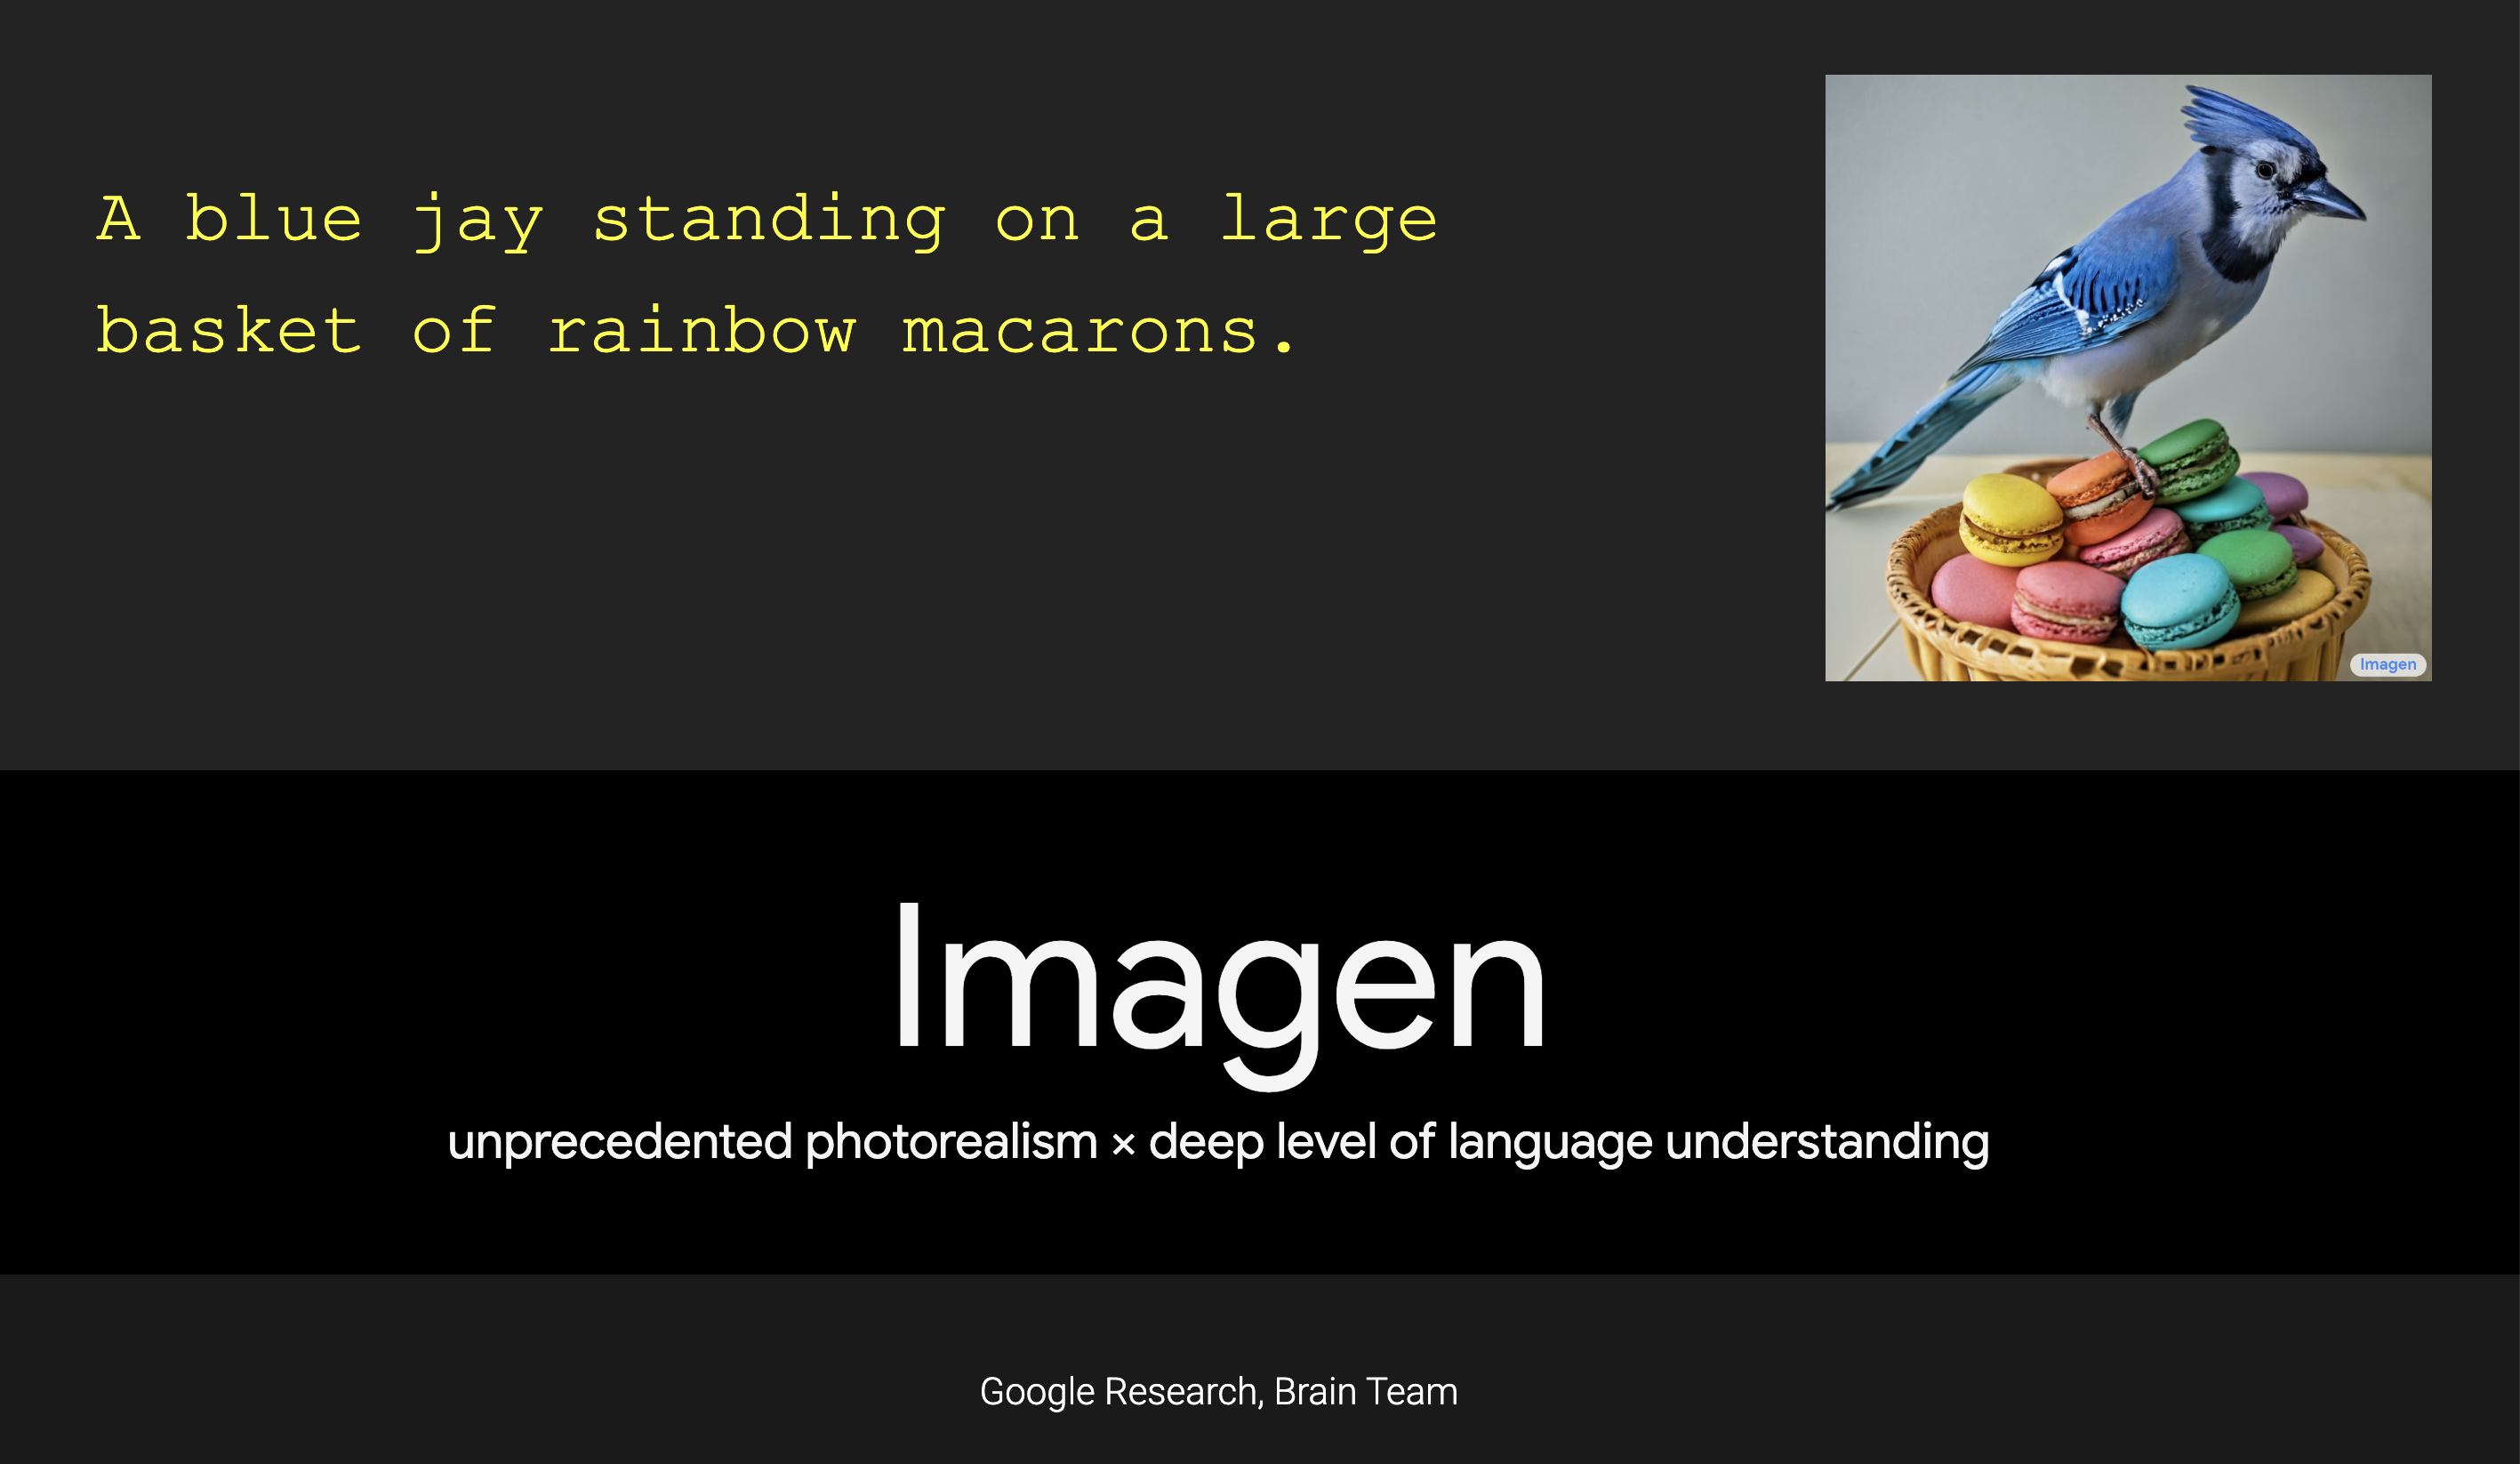
\includegraphics[width=.7\linewidth]{google_imgen.png}
	\end{center}
	\vfill
	\footnotesize  {\color{blue} \url{https://imagen.research.google/}} 
\end{frame} 



\begin{transitionframe}
	\begin{center}
		\Huge  История автоперевода
	\end{center}
\end{transitionframe}


\begin{frame}{Переводчики}
	\begin{center}
		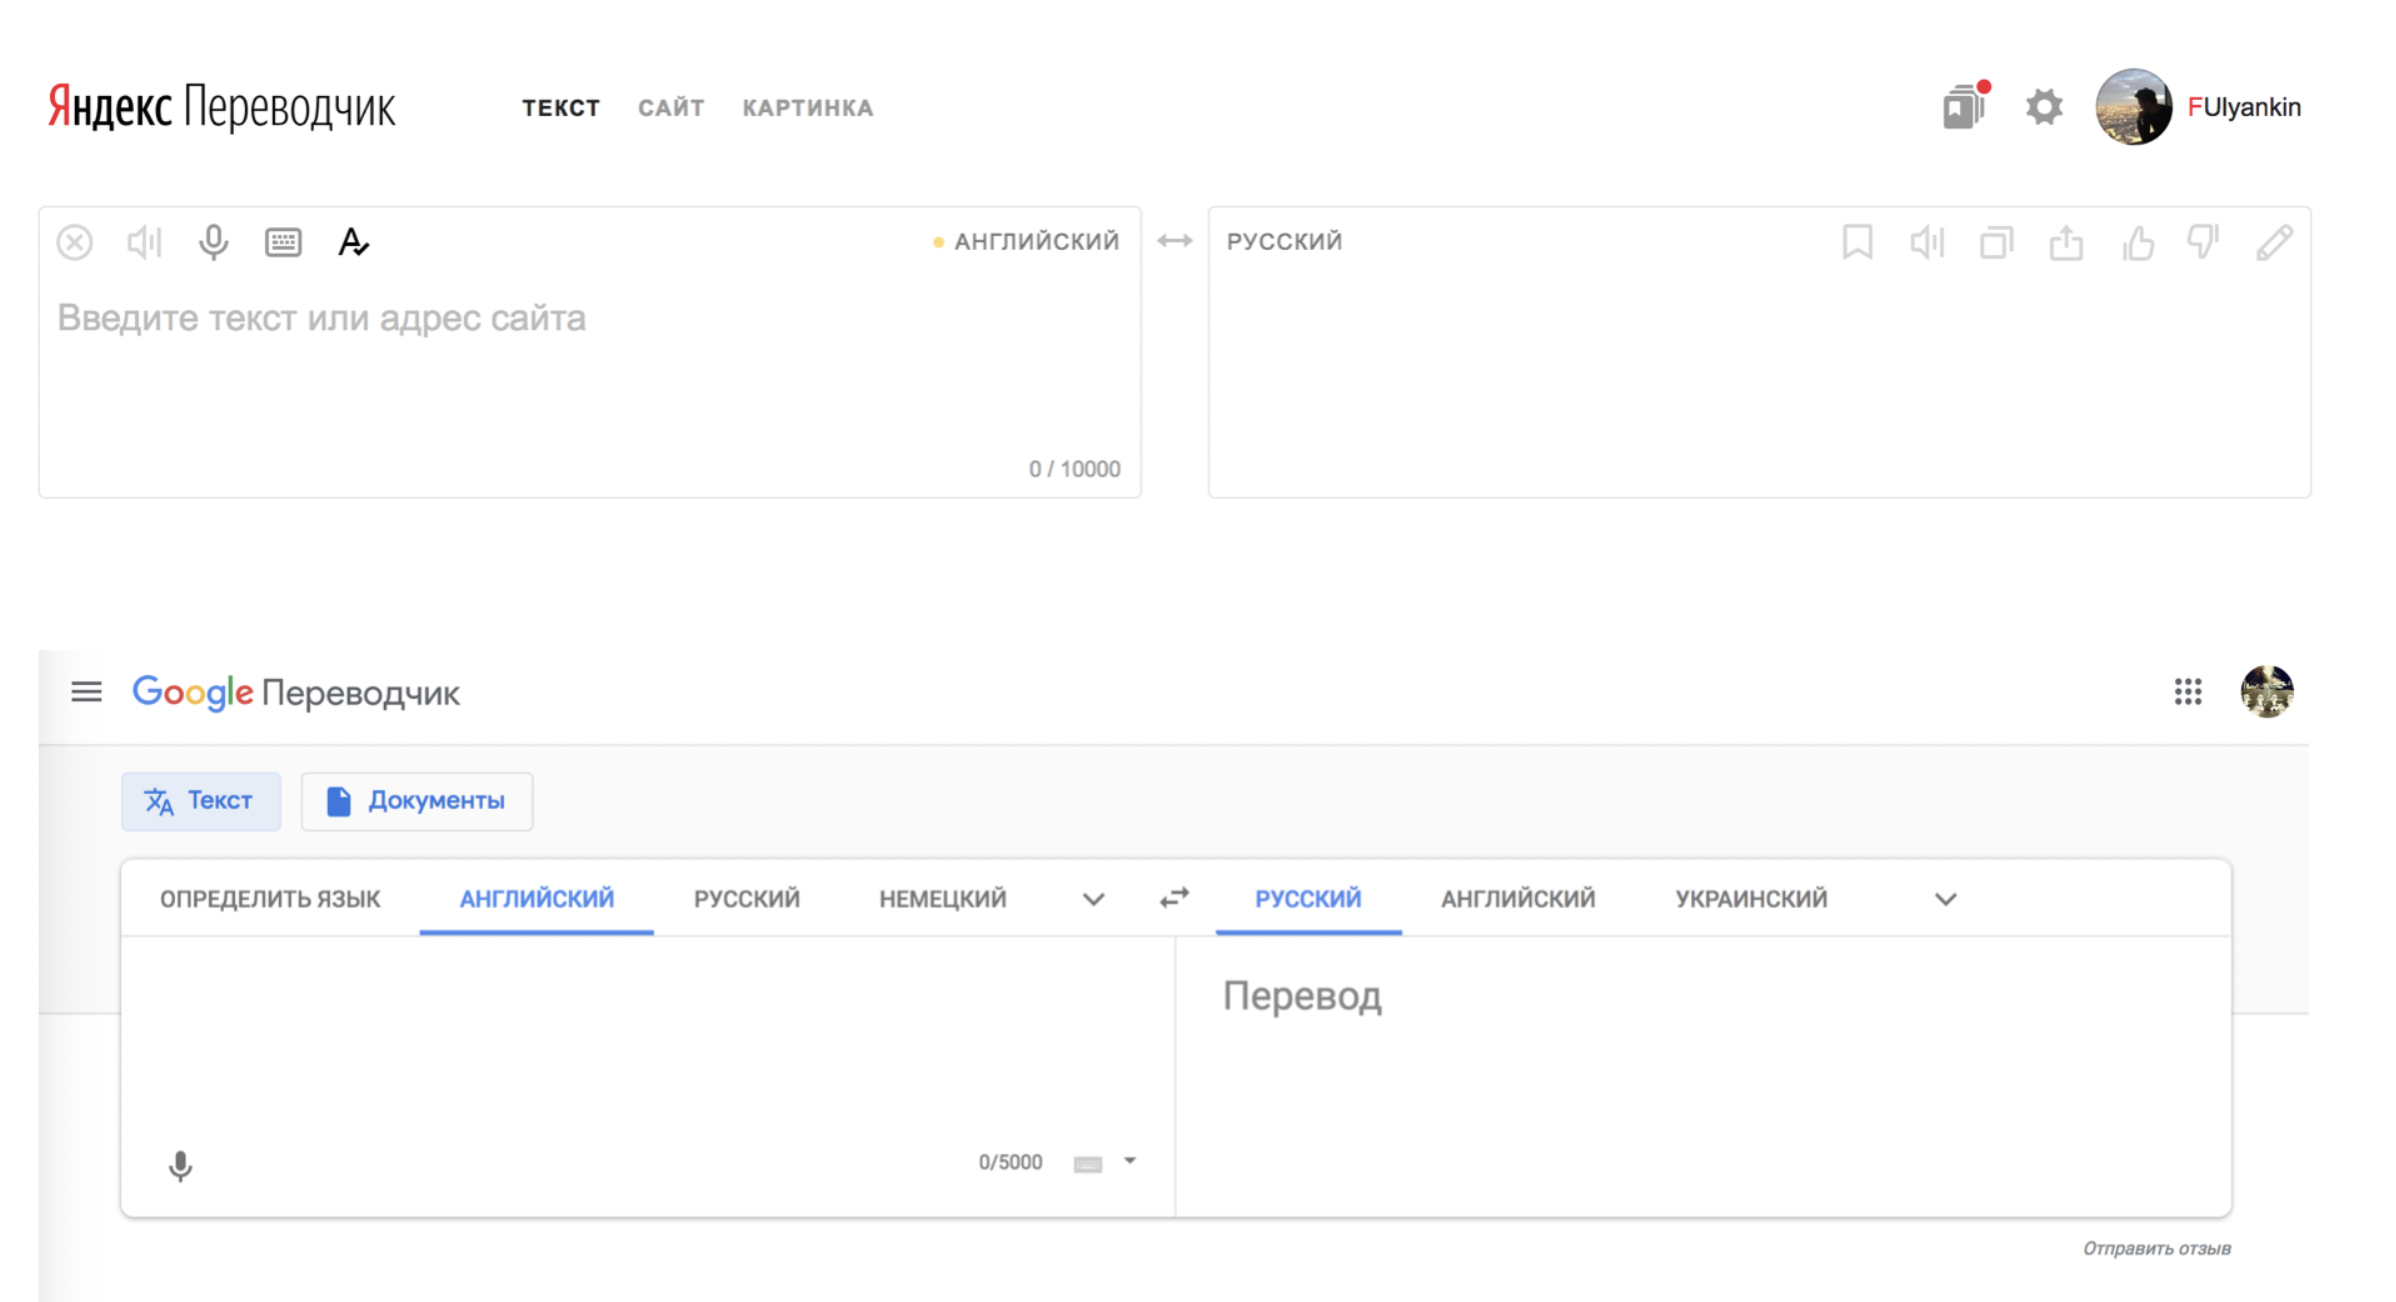
\includegraphics[width=.8\linewidth]{gy_tr.png}
	\end{center}
\end{frame} 


\begin{frame}{Кто и когда захотел}
	\begin{wideitemize} 
		\item  Холодная война, 1954 год. США и СССР хотят получить машину для автопереводов
		\item  Джорджтаунский эксперимент (IBM): перевод 60 предложений с перфокарт 
		\item  В СССР аналогичный эксперимент
		\item  В обоих государствах все предложения для перевода тщательно подобраны и оттестированы :(
	\end{wideitemize} 
	\vfill
\footnotesize  {\color{blue} \url{https://vas3k.ru/blog/machine_translation/}} 
\end{frame} 



\begin{frame}{Кто и когда захотел}
	\begin{wideitemize} 
		\item  Учёные обещают, что в течение ближайших 5 лет задача машинного перевода будет решена.
		\item  Через 12 лет, в 1966 американский комитет ALPAC публикует отчёт, в котором называет машинный перевод дорогим, неточным и бесперспективным
	\end{wideitemize} 
	\vfill
\footnotesize  {\color{blue} \url{https://vas3k.ru/blog/machine_translation/}} 
\end{frame} 


\begin{frame}{Rule-based machine translation, RBMT}
	\begin{wideitemize} 
		\item  Получает интенсивное развитие в 1970-х годах
		\item  Словари + попытка посмотреть на то как работают лингвисты и вбить какие-то паттерны в компьютер (существительные оканчиваются на а-я и тп)
		\item Бывает разных видов
	\end{wideitemize} 
	\vfill
\footnotesize  {\color{blue} \url{https://vas3k.ru/blog/machine_translation/}} 
\end{frame} 


\begin{frame}{Rule-based machine translation, RBMT}
	\begin{wideitemize} 
		\item   \alert{Дословный перевод (Direct Machine Translation):}  делим текст по словам, переводим каждое, правим каждое слово в соответствии с накопленными правилами (окончания, падежи и тп). Правила придумывают лингвисты.
		\item  \alert{Трансферные системы (Transfer-based Machine Translation):} сначала выделяем синтаксические конструкции (сказуемые, подлежащие и тп), понимаем как слова надо переставить, а потом уже переводим.
	\end{wideitemize} 
	\vfill
	\footnotesize  {\color{blue} \url{https://vas3k.ru/blog/machine_translation/}} 
\end{frame} 


\begin{frame}{Эти типы стали есть на складе}
	\begin{wideitemize} 
		\item  Придумывать правила вручную - сложно
		\item  Огромное количество исключений
		\item  Омонимия (разный смысл одних и тех же слов в зависимости от контекста)
		\item  RBMT системы за годы холодной войны вышли на пик и успешно умерли, сегодня они не используются нигде
	\end{wideitemize} 
	\vfill
	\footnotesize  {\color{blue} \url{https://vas3k.ru/blog/machine_translation/}} 
\end{frame} 


\begin{frame}{Statistical machine translation (SMT)}
	\begin{wideitemize} 
		\item  IBM, 1990 г.
		\item  Берём корпус параллельных текстов, смотрим как часто слово house
		переводится как дом, строение, постройка, так и переводим!
		\item  Работало лучше, чем всё что было до этого
	\end{wideitemize} 
	\vfill
	\footnotesize  {\color{blue} \url{https://vas3k.ru/blog/machine_translation/}} 
\end{frame} 


\begin{frame}{Statistical machine translation (SMT)}
	\begin{center}
		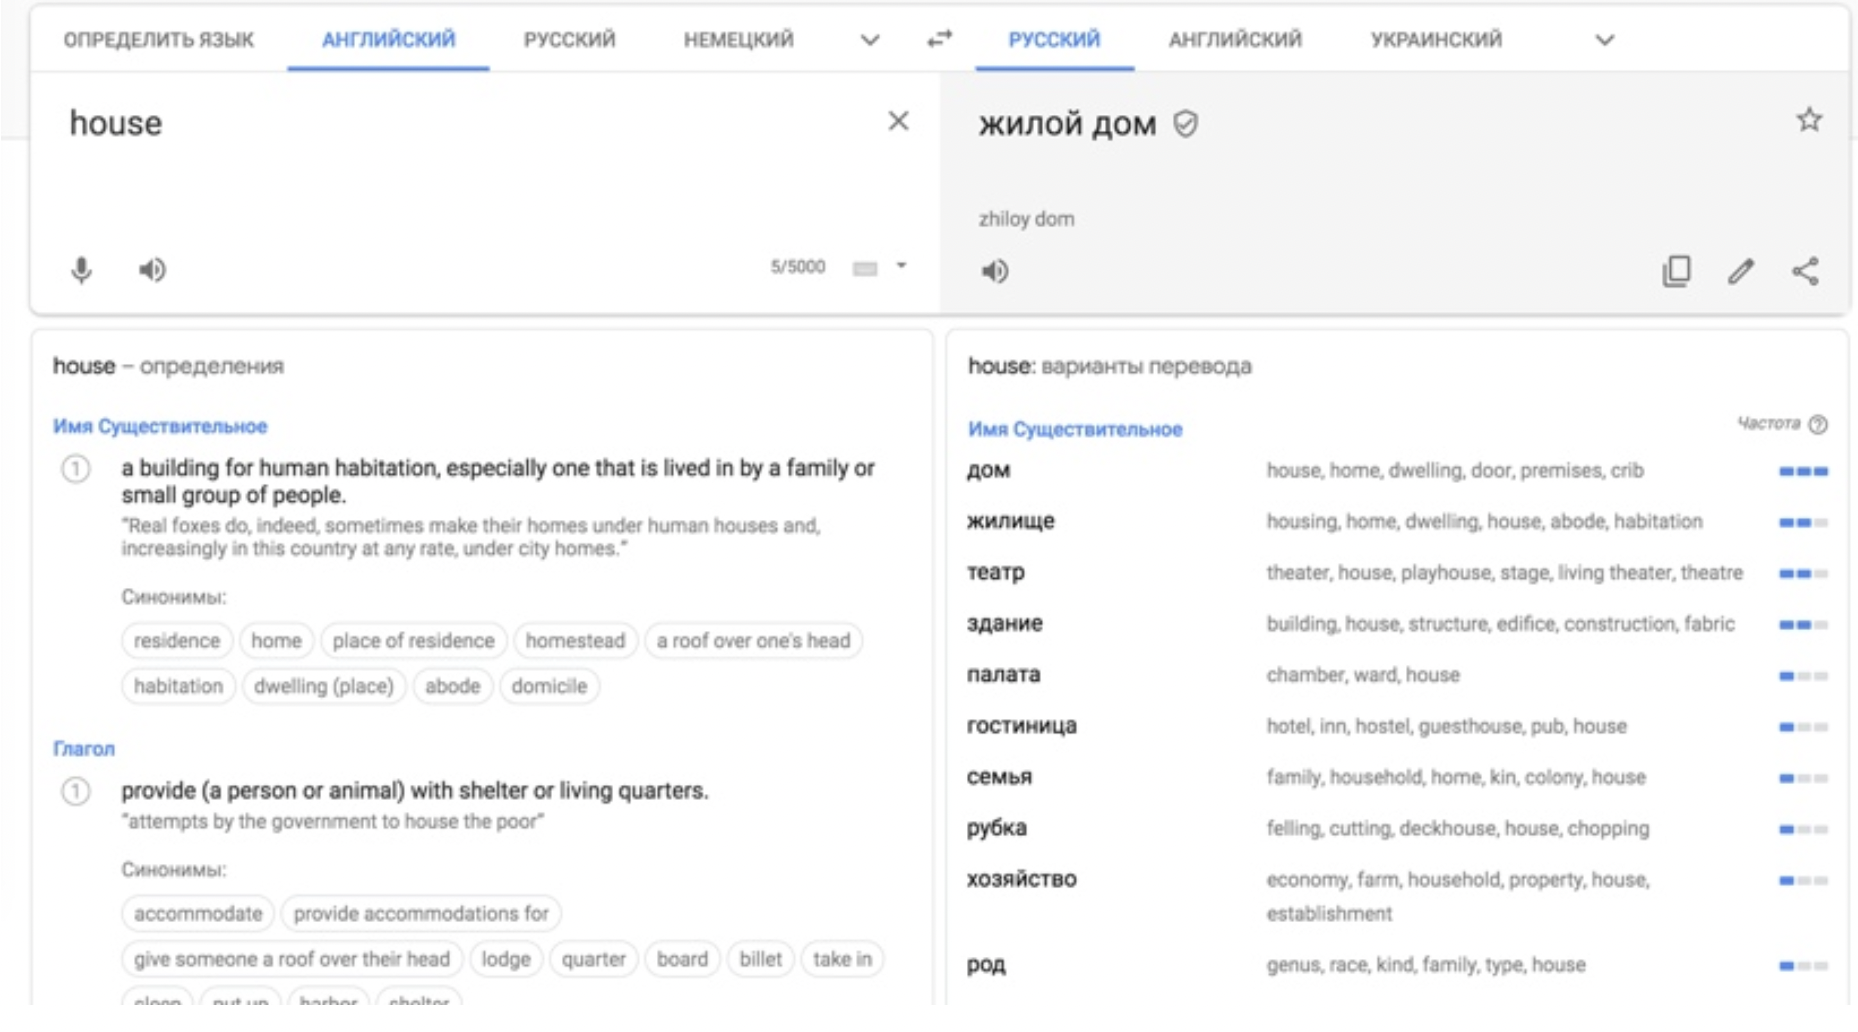
\includegraphics[width=.7\linewidth]{smt_ex.png}
	\end{center}
\end{frame} 


\begin{frame}{Word-based SMT}
	\begin{wideitemize} 
		\item  Начали конечно же со статистического перевода по отдельным словам
		\item  Пример реализации на python: \url{https://github.com/shawa/IBM-Model-1}
		\item  Дальше попробовали также по статистике переставлять слова, добавлять недостающие артикли
		\item  Всё ещё много проблем с омонимией и согласованностью слов в предложениях
	\end{wideitemize} 
	\vfill
	\footnotesize  {\color{blue} \url{https://vas3k.ru/blog/machine_translation/}} 
\end{frame} 


\begin{frame}{GTA San Andreas (2005) }
	\begin{center}
		
\includegraphics[width=.8\linewidth]{cj.png}
	\end{center}
\end{frame} 


\begin{frame}{Phrase-based SMT}
	\begin{wideitemize} 
		\item  Word-based SMT был основан на мешке слов, тут подмешали N-граммы
		\item  C 2006 года этот подход использовали абсолютно все
		\item  Так продолжалось до 2016 года
		\item  В 2016 году Google перевернул игру: \url{https://ai.googleblog.com/2016/09/a-neural-network-for-machine.html}
	\end{wideitemize} 
	\vfill
	\footnotesize  {\color{blue} \url{https://vas3k.ru/blog/machine_translation/}} 
\end{frame} 


\begin{transitionframe}
	\begin{center}
		\Huge  Нейросетевой перевод
	\end{center}
\end{transitionframe}


\begin{frame}{Энкодер для картинки}
	\begin{center}
		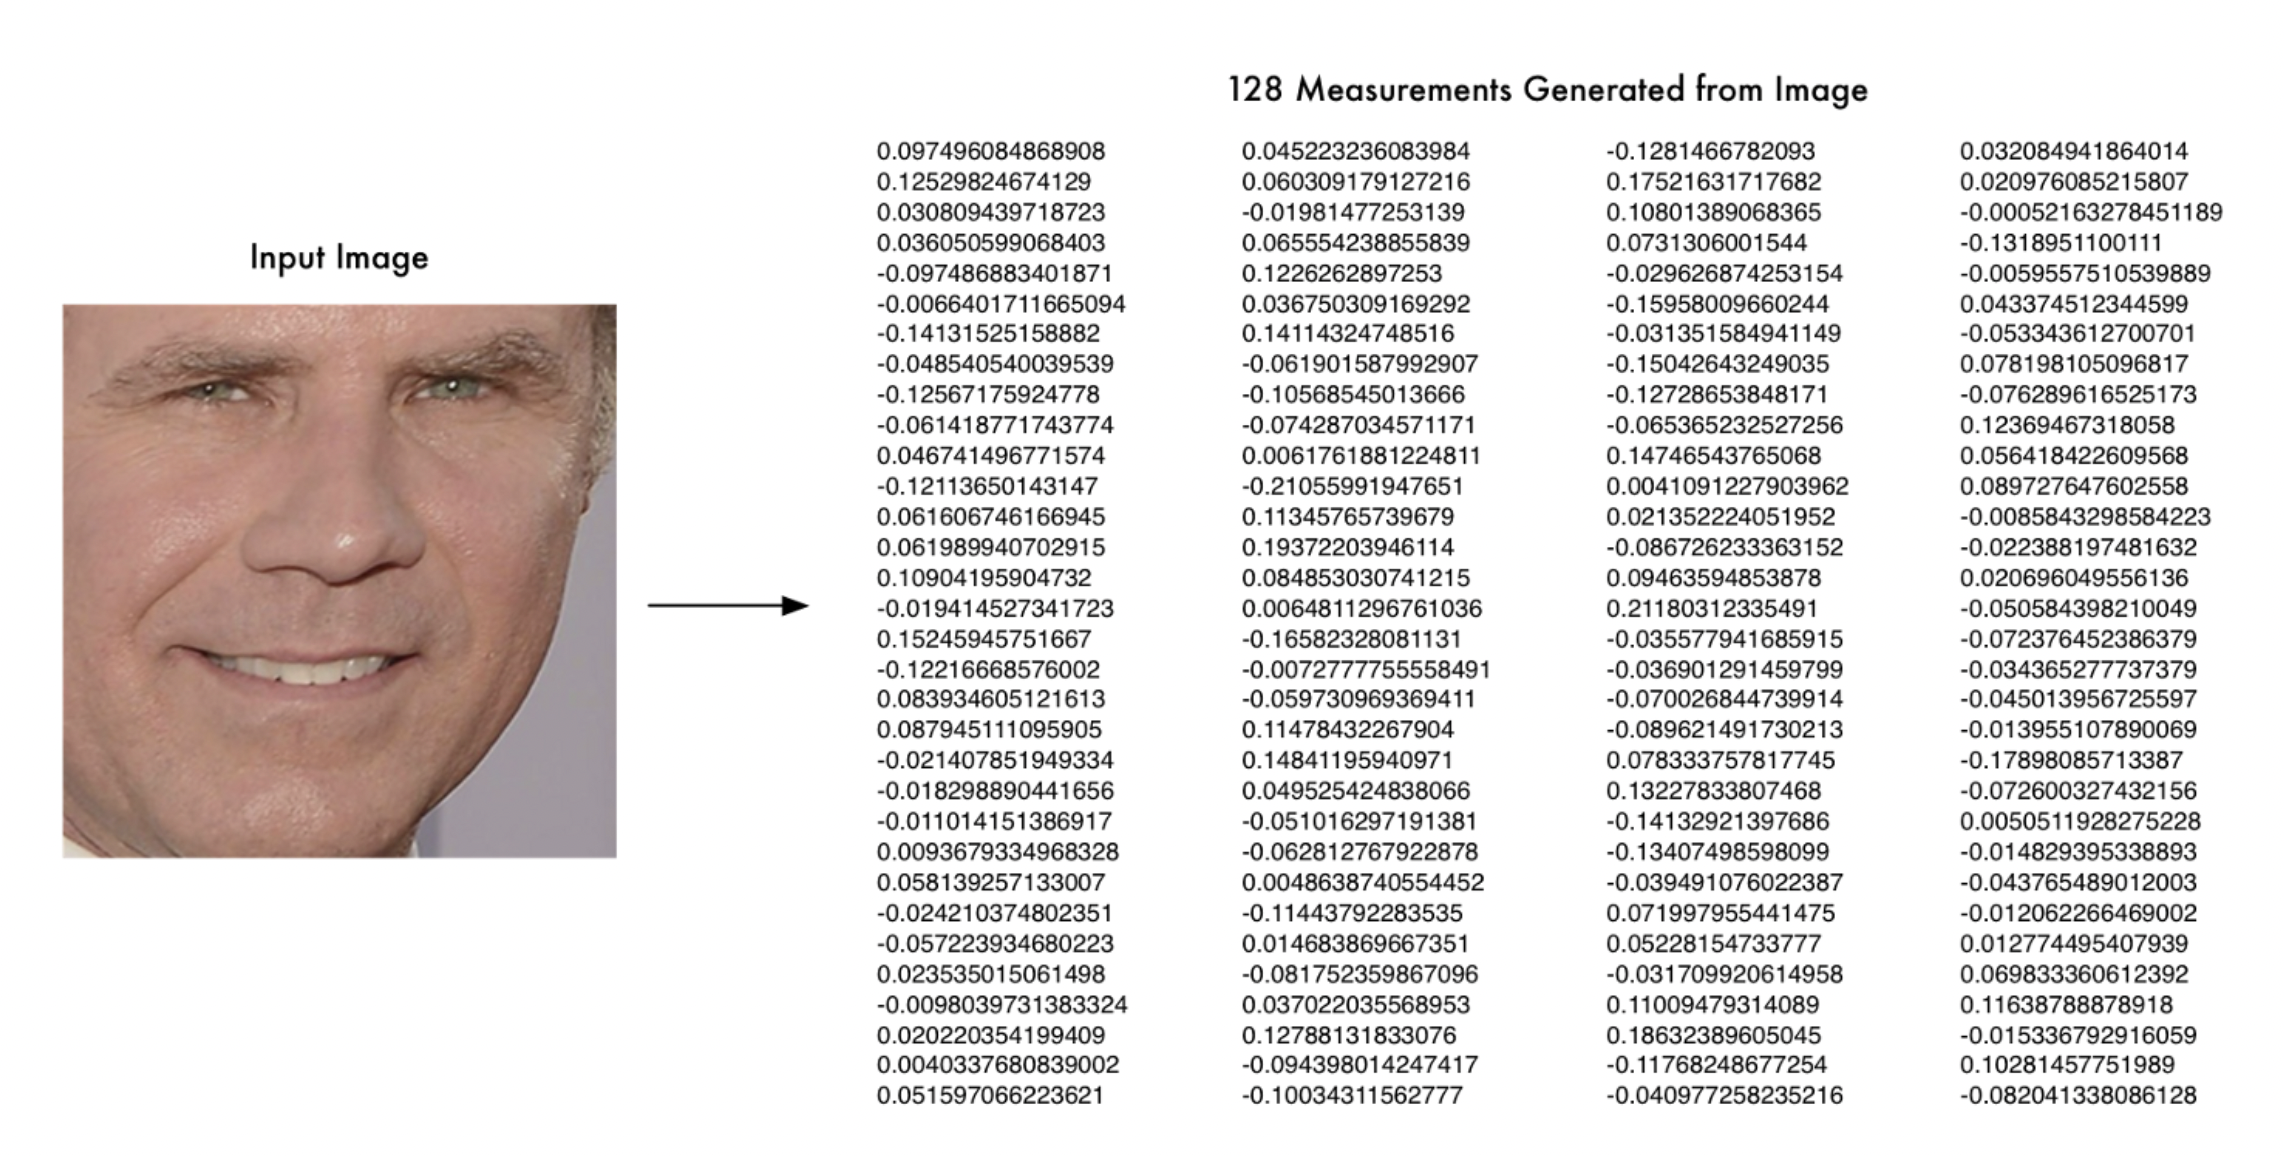
\includegraphics[width=.8\linewidth]{pic_text_face.png}
	\end{center}
\end{frame} 


\begin{frame}{Энкодер для текста}
	\begin{center}
		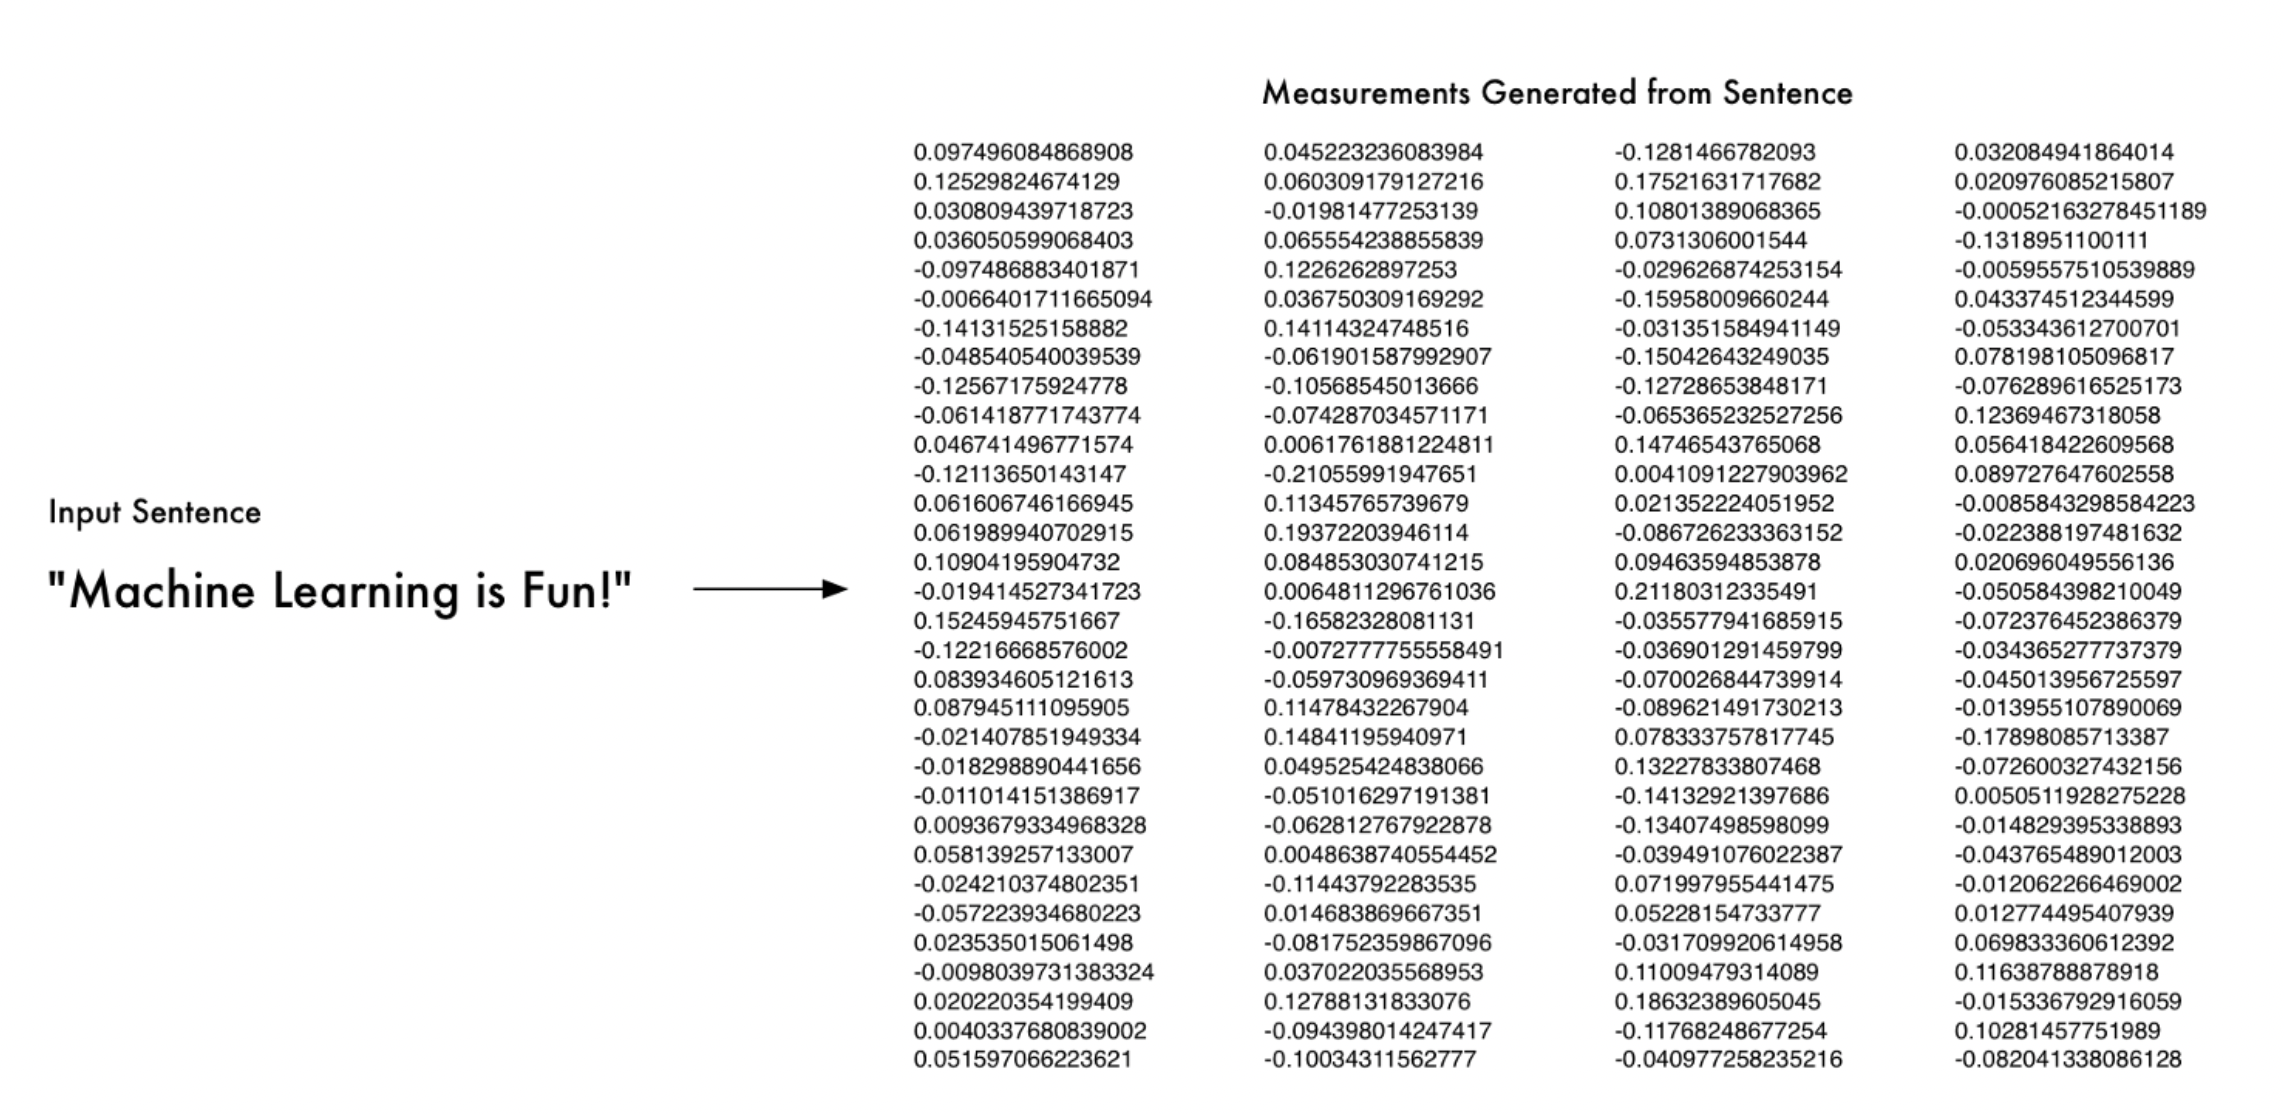
\includegraphics[width=.8\linewidth]{pic_text_text.png}
	\end{center}
\end{frame} 


\begin{frame}{Автокодировщик для текста}
	\begin{center}
		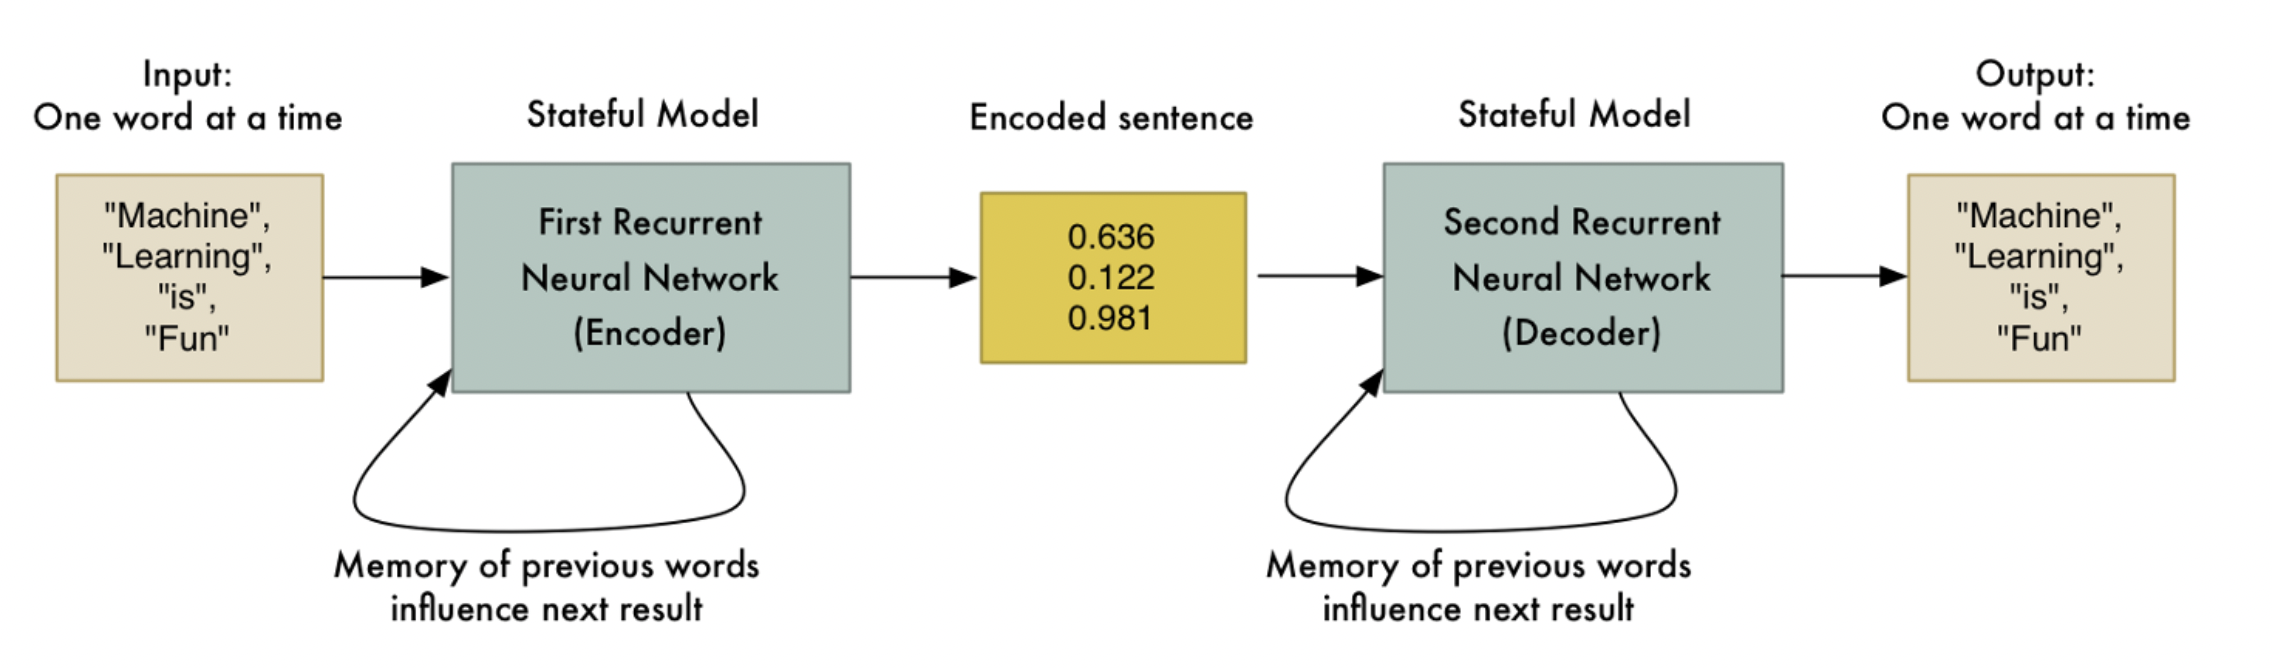
\includegraphics[width=.95\linewidth]{autoencoder_text.png}
	\end{center}
	\vfill
\footnotesize  {\color{blue} \url{https://medium.com/@ageitgey/build-your-own-google-translate-quality-machine-translation-system-d7dc274bd476}} 
\end{frame} 


\begin{frame}{Автокодировщик для текста}
	\begin{center}
		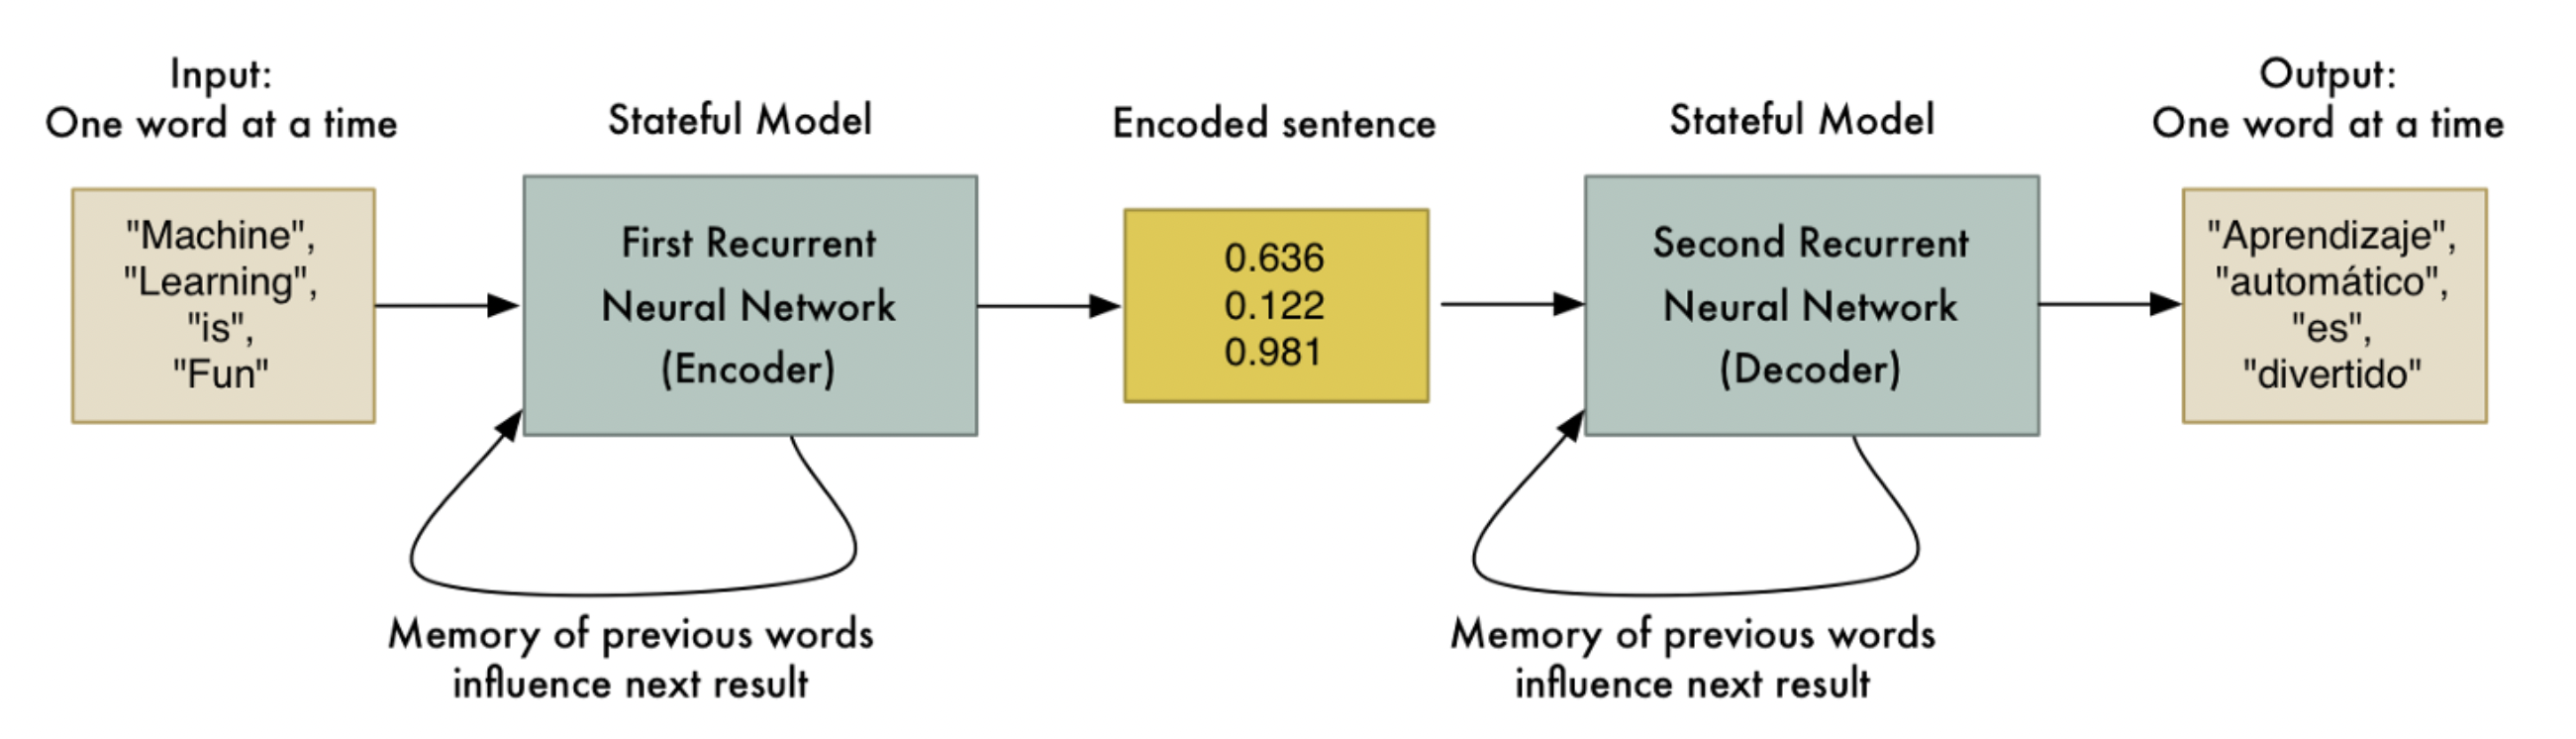
\includegraphics[width=.95\linewidth]{autoencoder_translater.png}
	\end{center}
	\vfill
	\footnotesize  {\color{blue} \url{https://medium.com/@ageitgey/build-your-own-google-translate-quality-machine-translation-system-d7dc274bd476}} 
\end{frame} 


\begin{frame}{Нейросетевые переводы}
	\begin{wideitemize} 
		\item  Энкодер пытается понять смысл и закодировать текст 
		\item  Декодер пытается раскодировать текст и сгенерировать таргет
	\end{wideitemize} 
\end{frame} 


\begin{frame}{Нейросетевые переводы}
	\begin{wideitemize} 
		\item  Архитектуры переводчиков очень разные
		\item  Поначалу это были RNN, после перешли на многослойные двунаправленные LSTM
		\item  Дальше стали пробовать разные виды эмбеддингов и механизмы внимания
		\item  Сегодня автопереводы делаются приемущественно трансформерами 
	\end{wideitemize} 
\end{frame} 


\begin{frame}{Нейросети + catboost}
	\begin{wideitemize} 
		\item  На коротких фразах нейросетевой перевод работает плохо
		\item  Перевод идёт двумя способами: статистическим и нейросетевым, а после Catboost выбирает тот, который лучше подходит
		\item  Пресс-релиз Яндекса от 2017:  \url{https://yandex.ru/blog/company/ kak-pobedit-mornikov-yandeks-zapustil-gibridnuyu-sistemu-perevoda}
		\item  - Статья Яндекса на хабре про историю автоперевода: \url{https://habr.com/ru/company/yandex/blog/224445/}
	\end{wideitemize} 
\end{frame} 



\begin{frame}{Простейшая модель: RNN энкодер-декодер}
	\begin{center}
		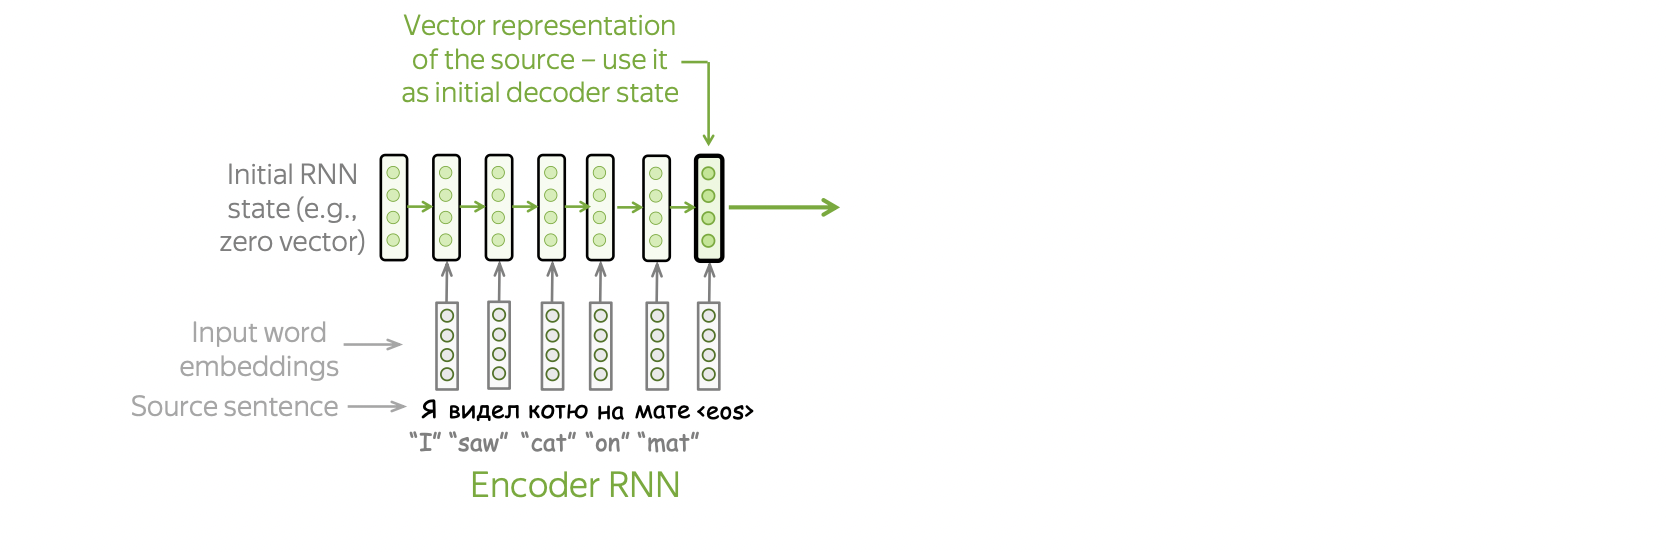
\includegraphics[width=.99\linewidth]{rnn_enc_1.png}
	\end{center}
	\vfill
	\footnotesize  {\color{blue} \url{https://github.com/yandexdataschool/nlp_course/tree/2021/week04_seq2seq}} 
\end{frame} 


\begin{frame}{Простейшая модель: RNN энкодер-декодер}
	\begin{center}
		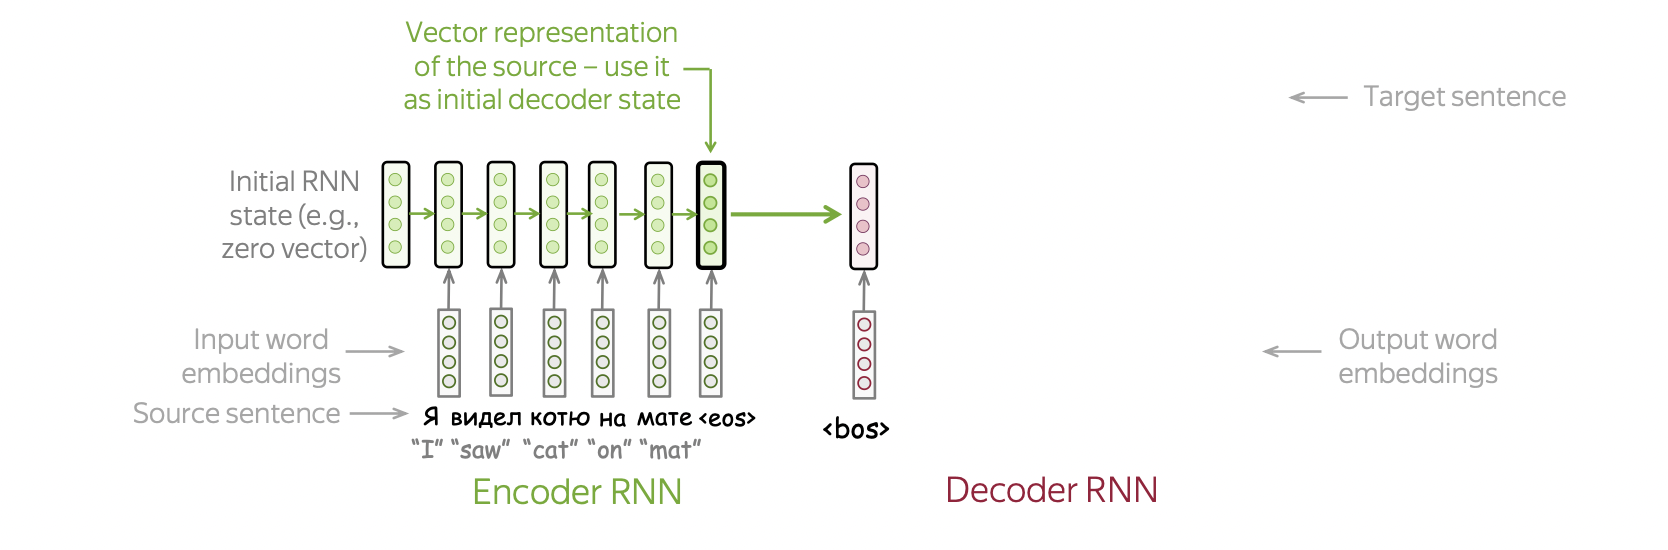
\includegraphics[width=.99\linewidth]{rnn_enc_2.png}
	\end{center}
	\vfill
	\footnotesize  {\color{blue} \url{https://github.com/yandexdataschool/nlp_course/tree/2021/week04_seq2seq}} 
\end{frame} 


\begin{frame}{Простейшая модель: RNN энкодер-декодер}
	\begin{center}
		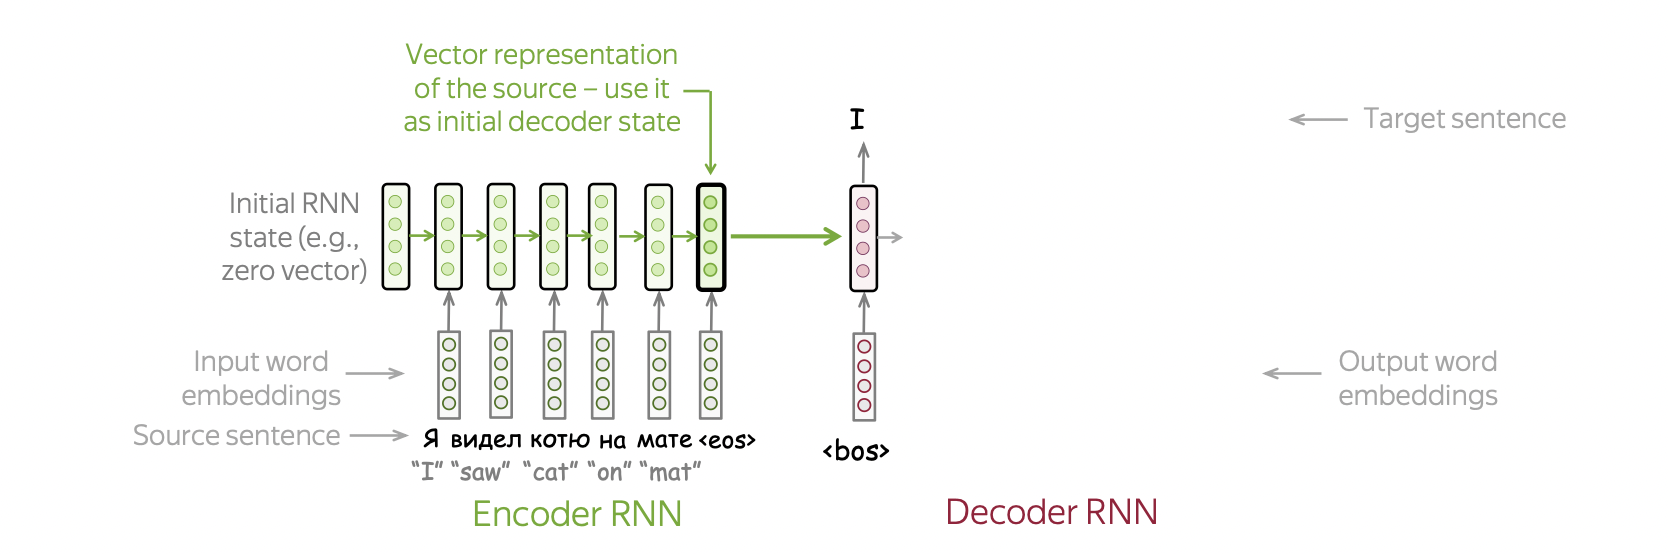
\includegraphics[width=.99\linewidth]{rnn_enc_3.png}
	\end{center}
	\vfill
	\footnotesize  {\color{blue} \url{https://github.com/yandexdataschool/nlp_course/tree/2021/week04_seq2seq}} 
\end{frame} 


\begin{frame}{Простейшая модель: RNN энкодер-декодер}
	\begin{center}
		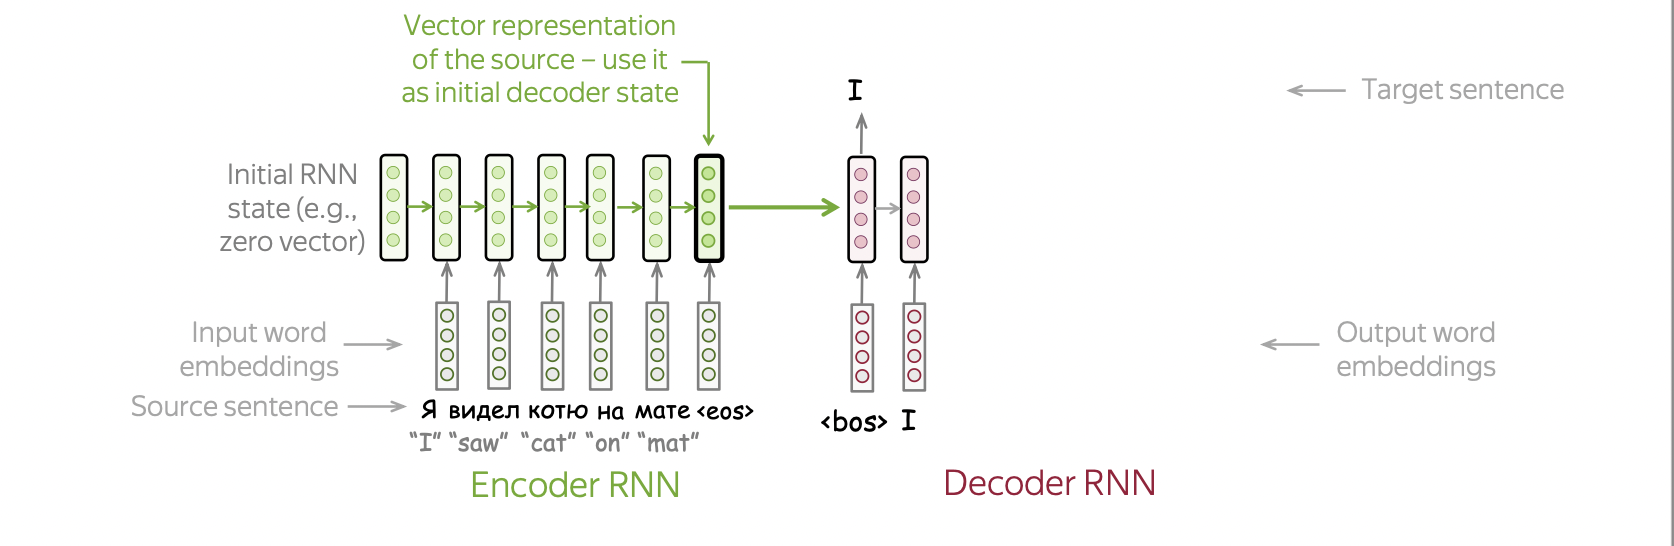
\includegraphics[width=.99\linewidth]{rnn_enc_4.png}
	\end{center}
	\vfill
	\footnotesize  {\color{blue} \url{https://github.com/yandexdataschool/nlp_course/tree/2021/week04_seq2seq}} 
\end{frame} 


\begin{frame}{Простейшая модель: RNN энкодер-декодер}
	\begin{center}
		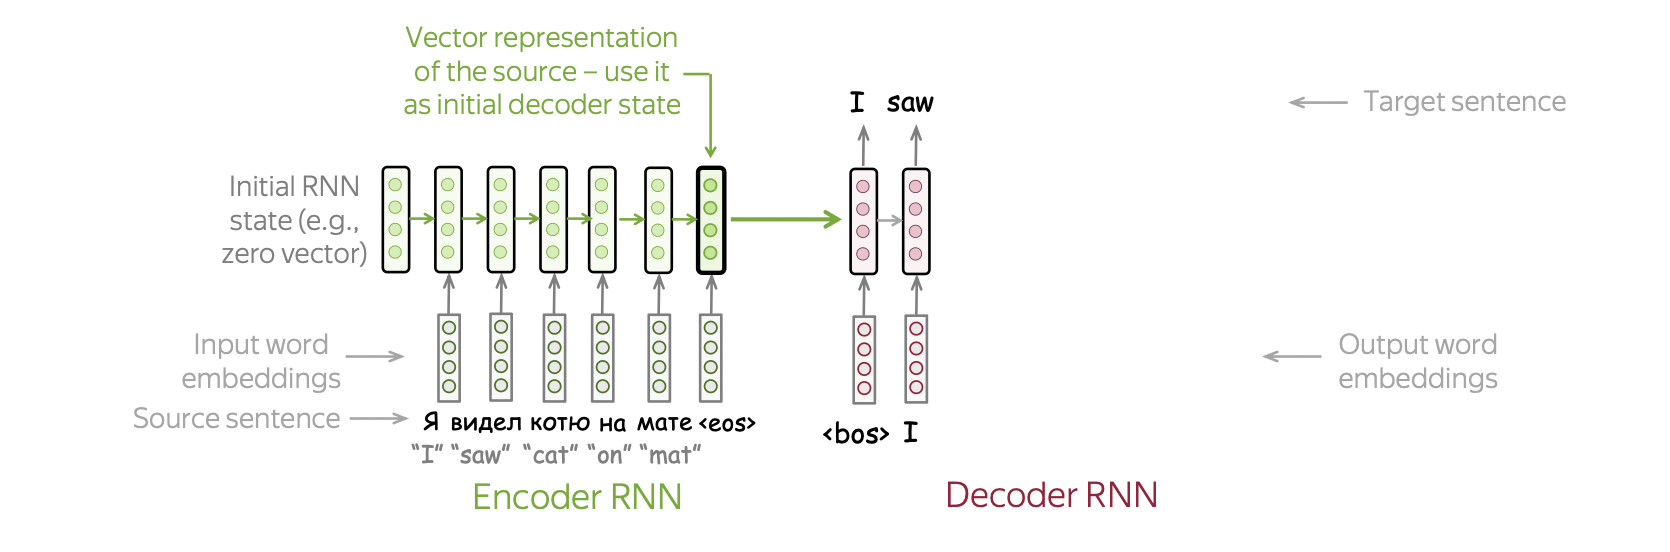
\includegraphics[width=.99\linewidth]{rnn_enc_5.png}
	\end{center}
	\vfill
	\footnotesize  {\color{blue} \url{https://github.com/yandexdataschool/nlp_course/tree/2021/week04_seq2seq}} 
\end{frame} 


\begin{frame}{Простейшая модель: RNN энкодер-декодер}
	\begin{center}
		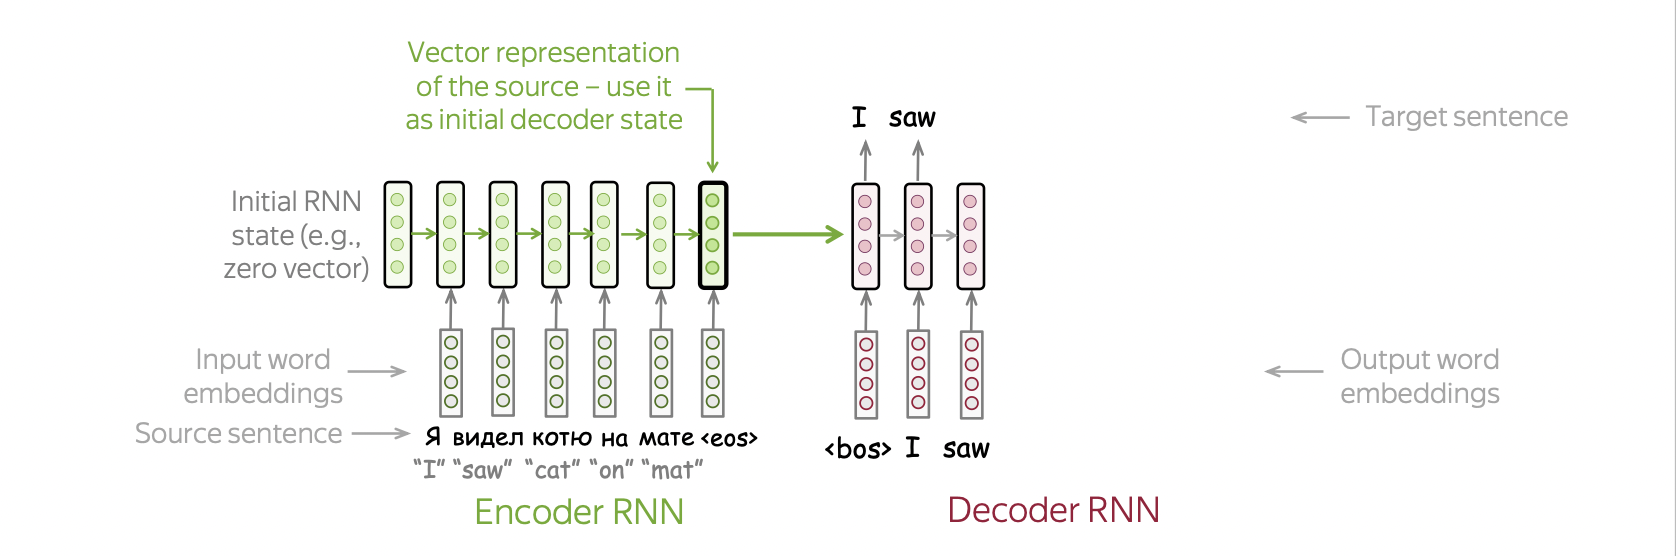
\includegraphics[width=.99\linewidth]{rnn_enc_6.png}
	\end{center}
	\vfill
	\footnotesize  {\color{blue} \url{https://github.com/yandexdataschool/nlp_course/tree/2021/week04_seq2seq}} 
\end{frame} 


\begin{frame}{Простейшая модель: RNN энкодер-декодер}
	\begin{center}
		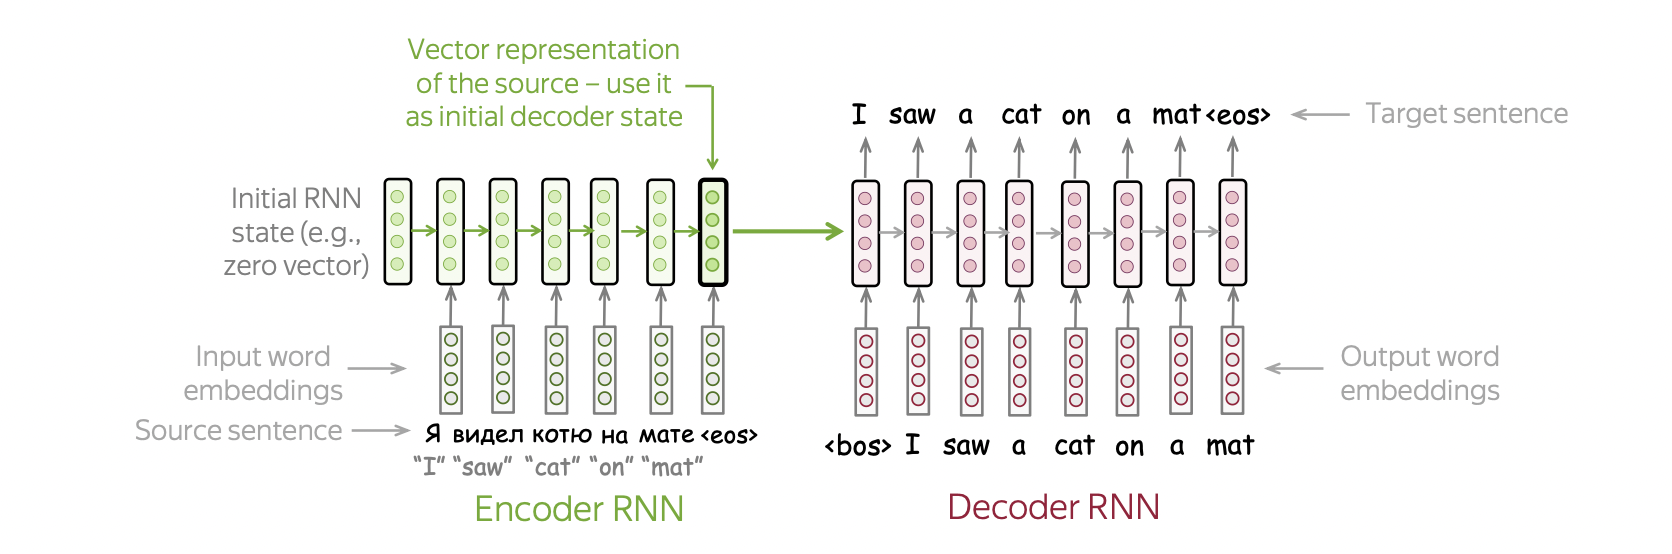
\includegraphics[width=.99\linewidth]{rnn_enc_7.png}
	\end{center}
	\vfill
	\footnotesize  {\color{blue} \url{https://github.com/yandexdataschool/nlp_course/tree/2021/week04_seq2seq}} 
\end{frame} 



\begin{frame}{Как обучить модель?}
	\begin{center}
		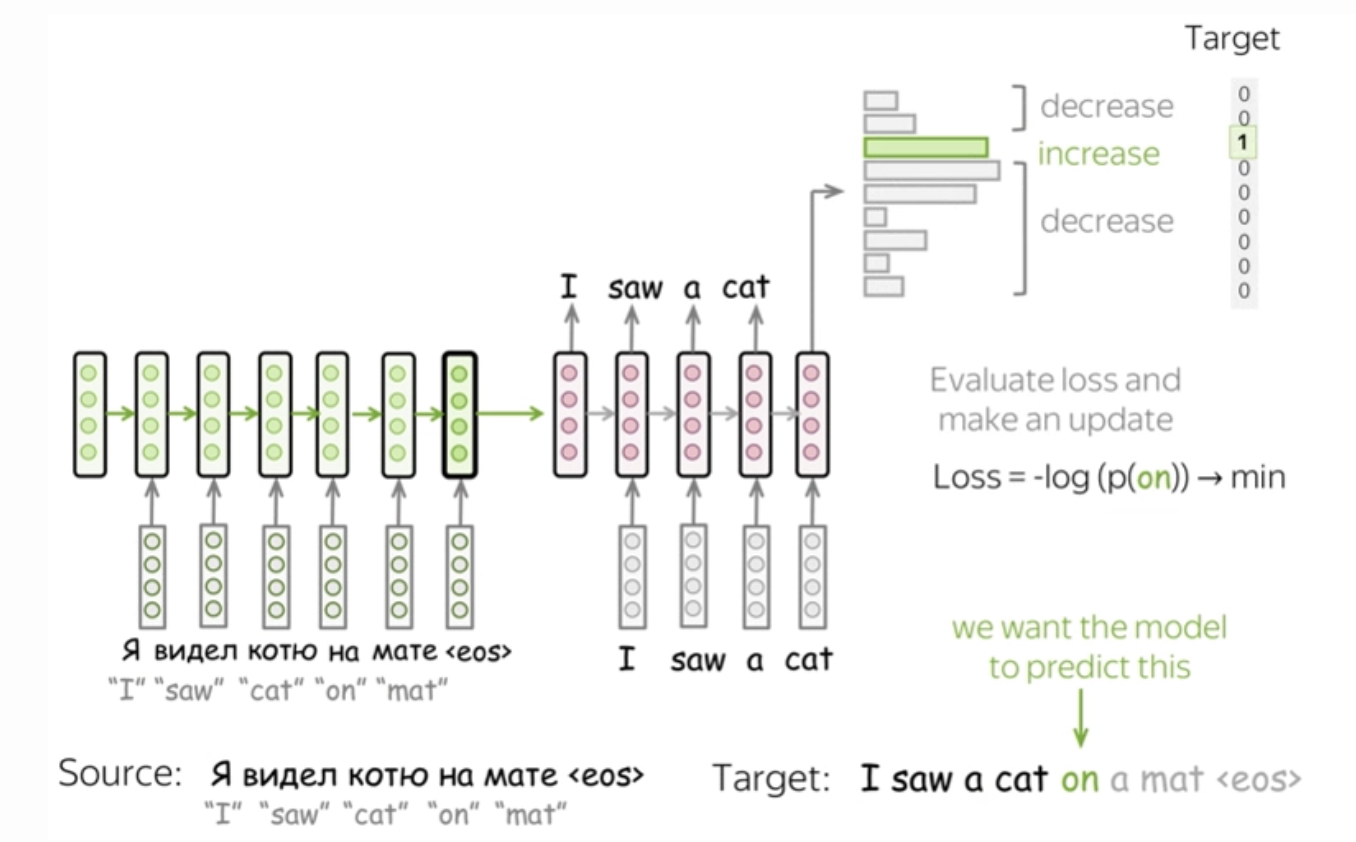
\includegraphics[width=.65\linewidth]{model_learn.png}
	\end{center}
	\vfill
	\scriptsize  {\color{blue} \url{https://lena-voita.github.io/resources/lectures/seq2seq/general/seq2seq_training_with_target.mp4}} 
\end{frame} 


\begin{frame}{Как сделать прогноз?}
	\begin{wideitemize} 
		\item  \alert{Жадно (greedy decoding):}  на каждом шаге берём токен с самой большой вероятностью
		
		\[ 
		\prod_{t=1}^T \arg \max_{y_t} p(y_t \mid y_{<t}, x)  \ne  \arg \max_{y}  \prod_{t=1}^T p(y_t \mid y_{<t}, x) 
		\]
		
		\item  Наш прогноз это последовательность, жадный способ на каждом шаге выбирает локальный оптимум
		
		\item  Перебирать все траектории, чтобы найти глобальный оптимум очень дорого
	\end{wideitemize} 

\end{frame} 

\begin{frame}{Неоптимальность Greedy Decoding}
	\begin{center}
			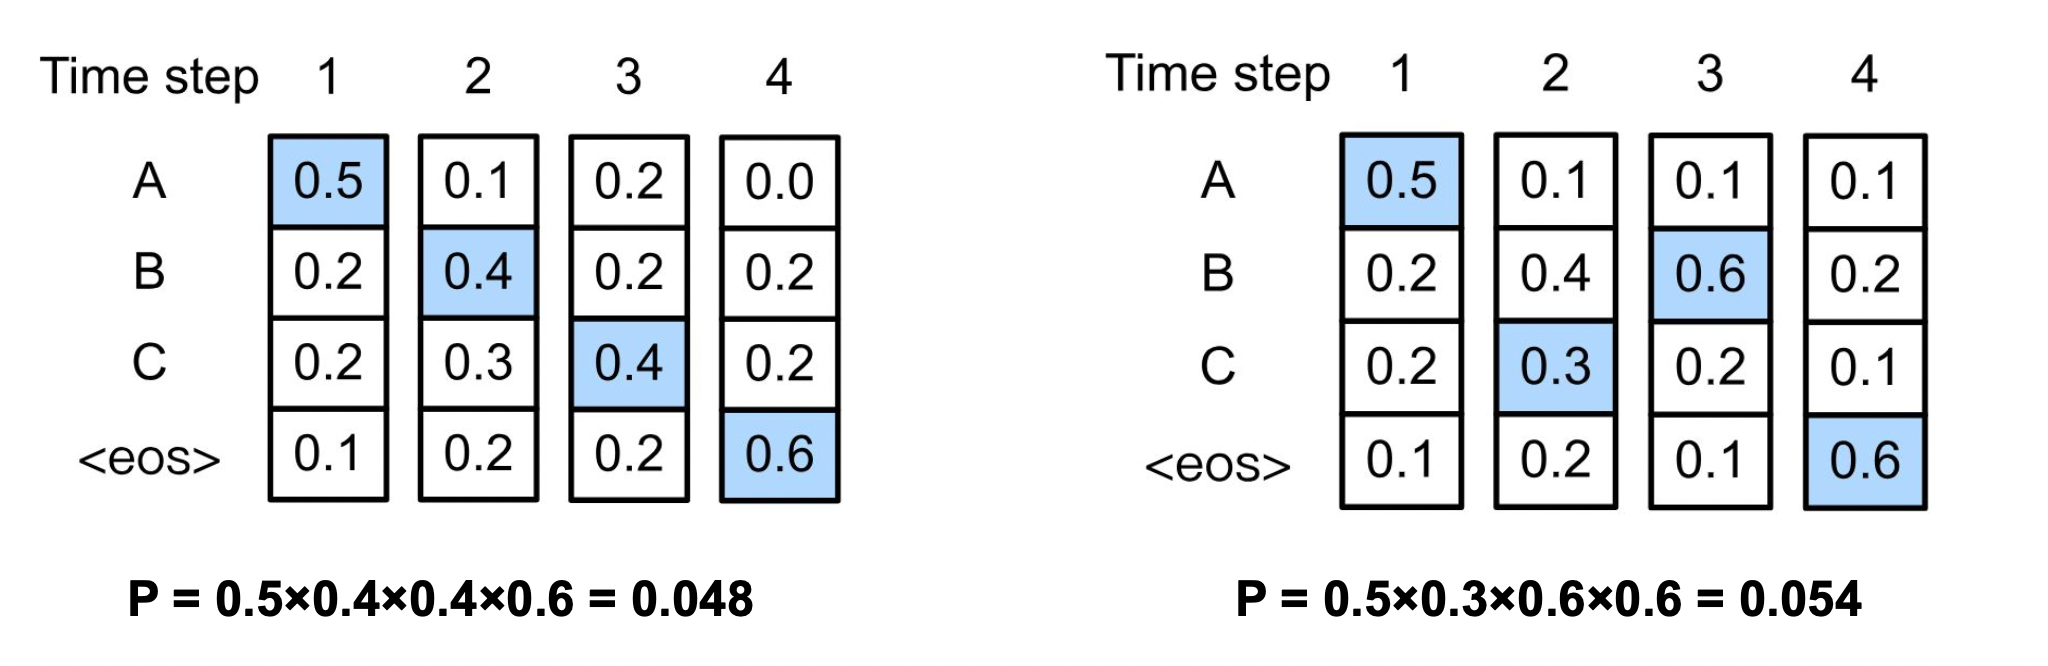
\includegraphics[width=.8\linewidth]{search.png}
	\end{center}
\end{frame} 


\begin{frame}{Beam Search}
	\begin{wideitemize} 	
			\item  Давайте поддерживать несколько самых вероятных траекторий
			\item  Такая стратегия называется \alert{Beam Search}
			\item  Число траекторий, которое мы помним будет гиперпараметром (больше $10$ брать не стоит)
	\end{wideitemize} 
\end{frame} 



\begin{frame}{Beam Search}
	\begin{center}
		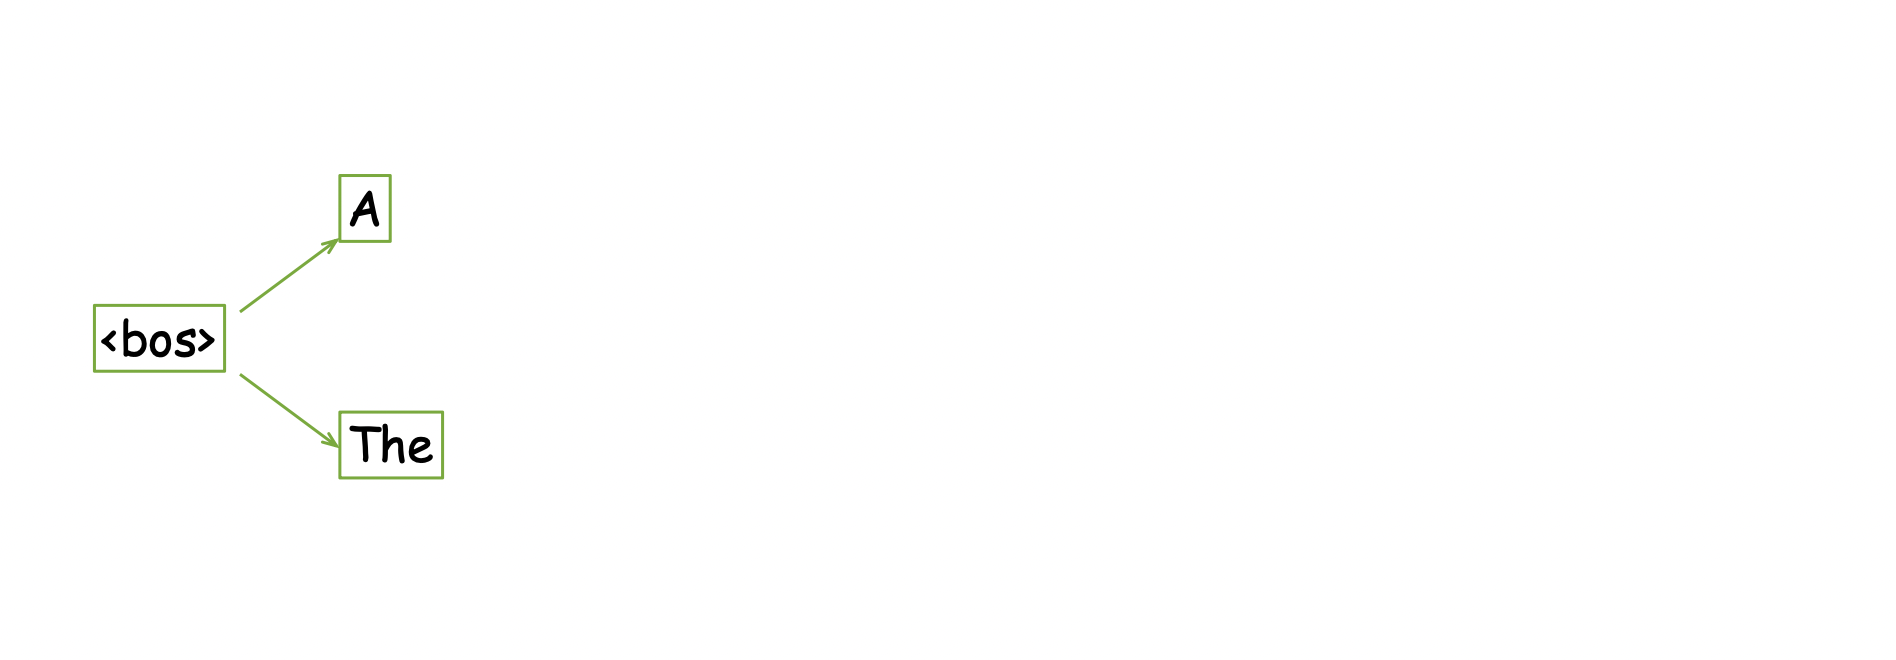
\includegraphics[width=.99\linewidth]{bs1.png}
	\end{center}
	\vfill
	\footnotesize  {\color{blue} \url{https://github.com/yandexdataschool/nlp_course/tree/2021/week04_seq2seq}} 
\end{frame} 

\begin{frame}{Beam Search}
	\begin{center}
		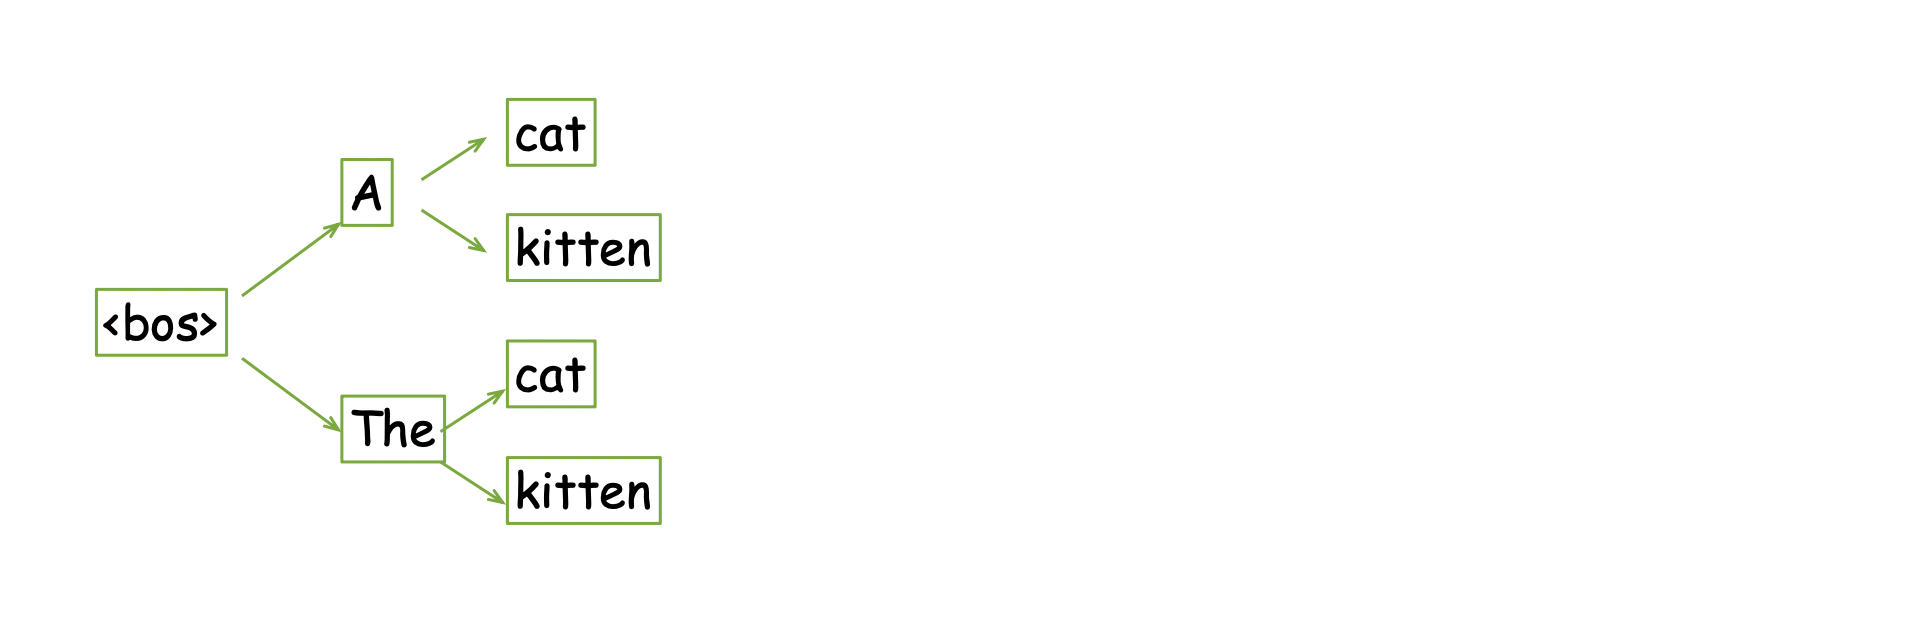
\includegraphics[width=.99\linewidth]{bs2.png}
	\end{center}
	\vfill
	\footnotesize  {\color{blue} \url{https://github.com/yandexdataschool/nlp_course/tree/2021/week04_seq2seq}} 
\end{frame} 

\begin{frame}{Beam Search}
	\begin{center}
		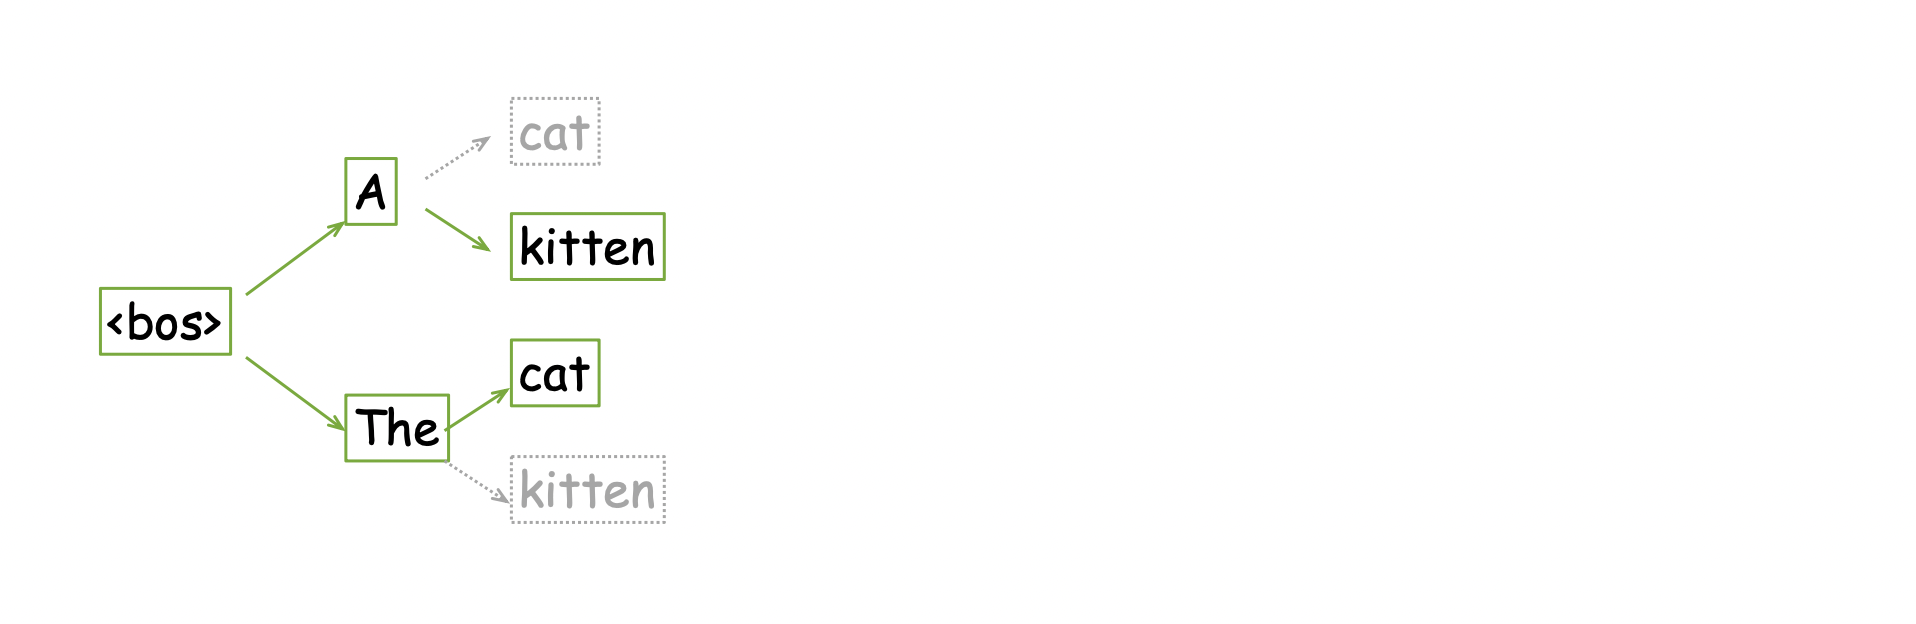
\includegraphics[width=.99\linewidth]{bs4.png}
	\end{center}
	\vfill
	\footnotesize  {\color{blue} \url{https://github.com/yandexdataschool/nlp_course/tree/2021/week04_seq2seq}} 
\end{frame} 

\begin{frame}{Beam Search}
	\begin{center}
		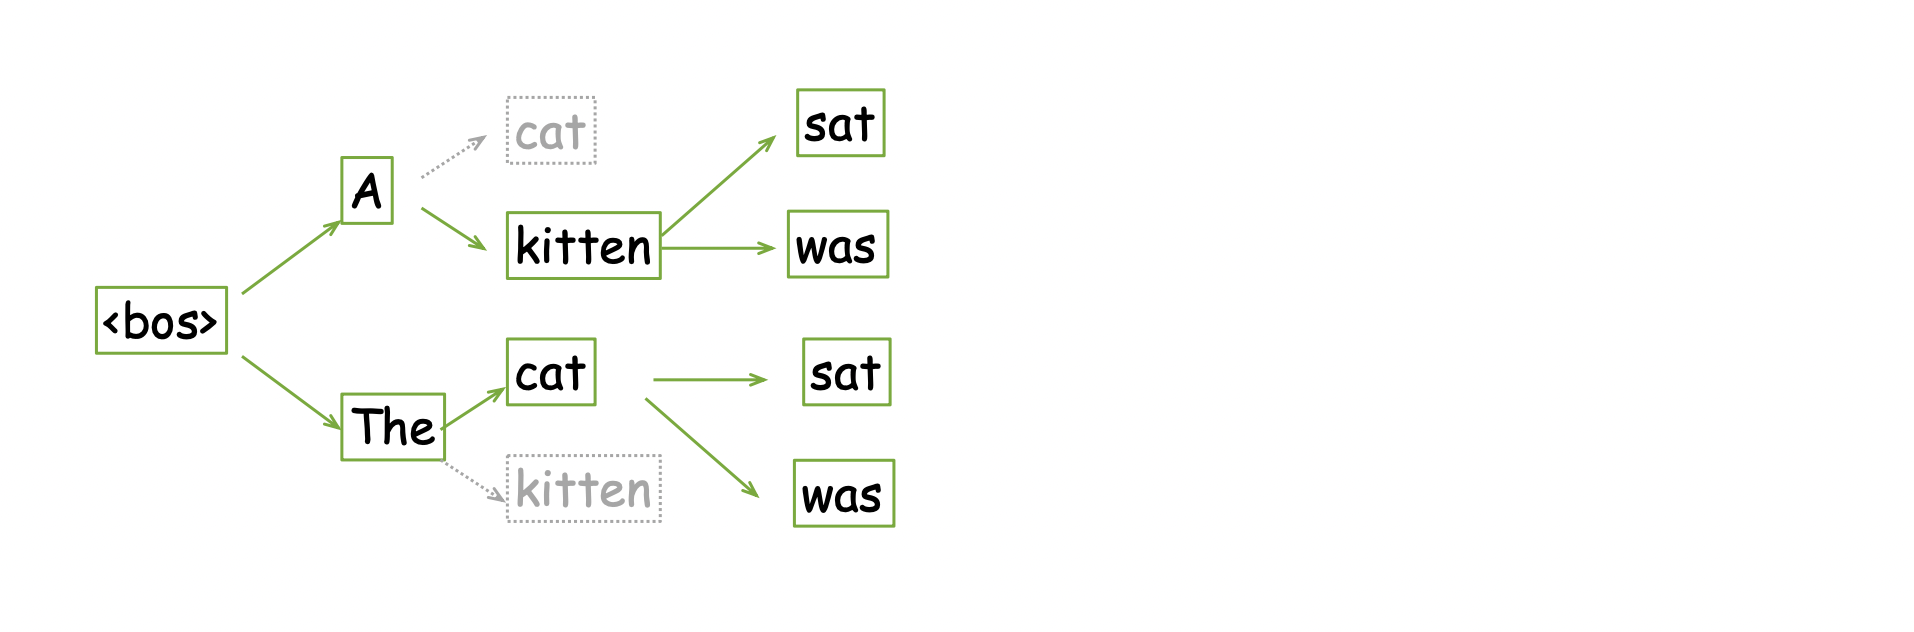
\includegraphics[width=.99\linewidth]{bs5.png}
	\end{center}
	\vfill
	\footnotesize  {\color{blue} \url{https://github.com/yandexdataschool/nlp_course/tree/2021/week04_seq2seq}} 
\end{frame} 

\begin{frame}{Beam Search}
	\begin{center}
		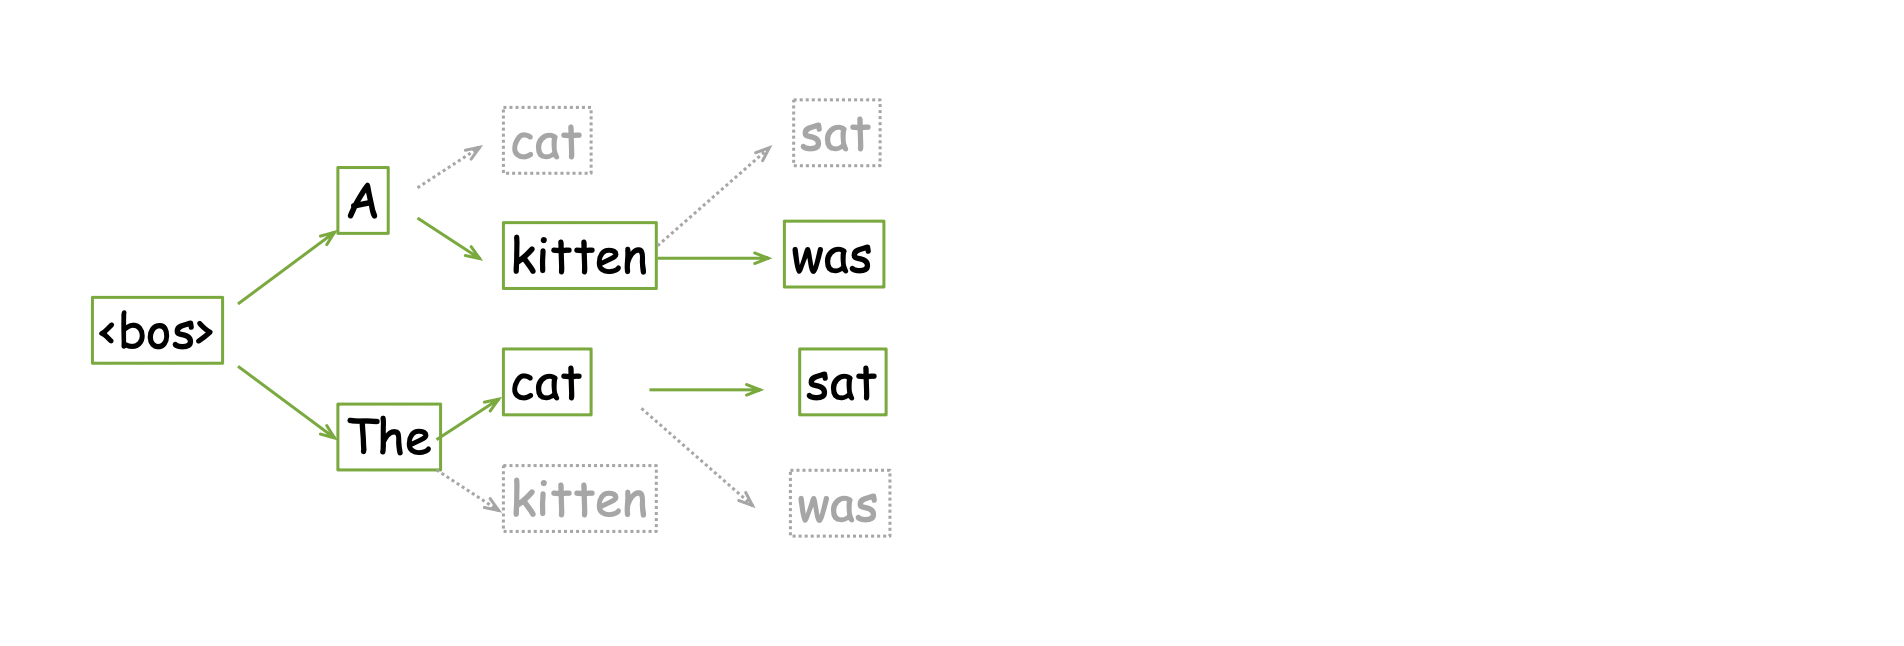
\includegraphics[width=.99\linewidth]{bs6.png}
	\end{center}
	\vfill
	\footnotesize  {\color{blue} \url{https://github.com/yandexdataschool/nlp_course/tree/2021/week04_seq2seq}} 
\end{frame} 

\begin{frame}{Beam Search}
	\begin{center}
		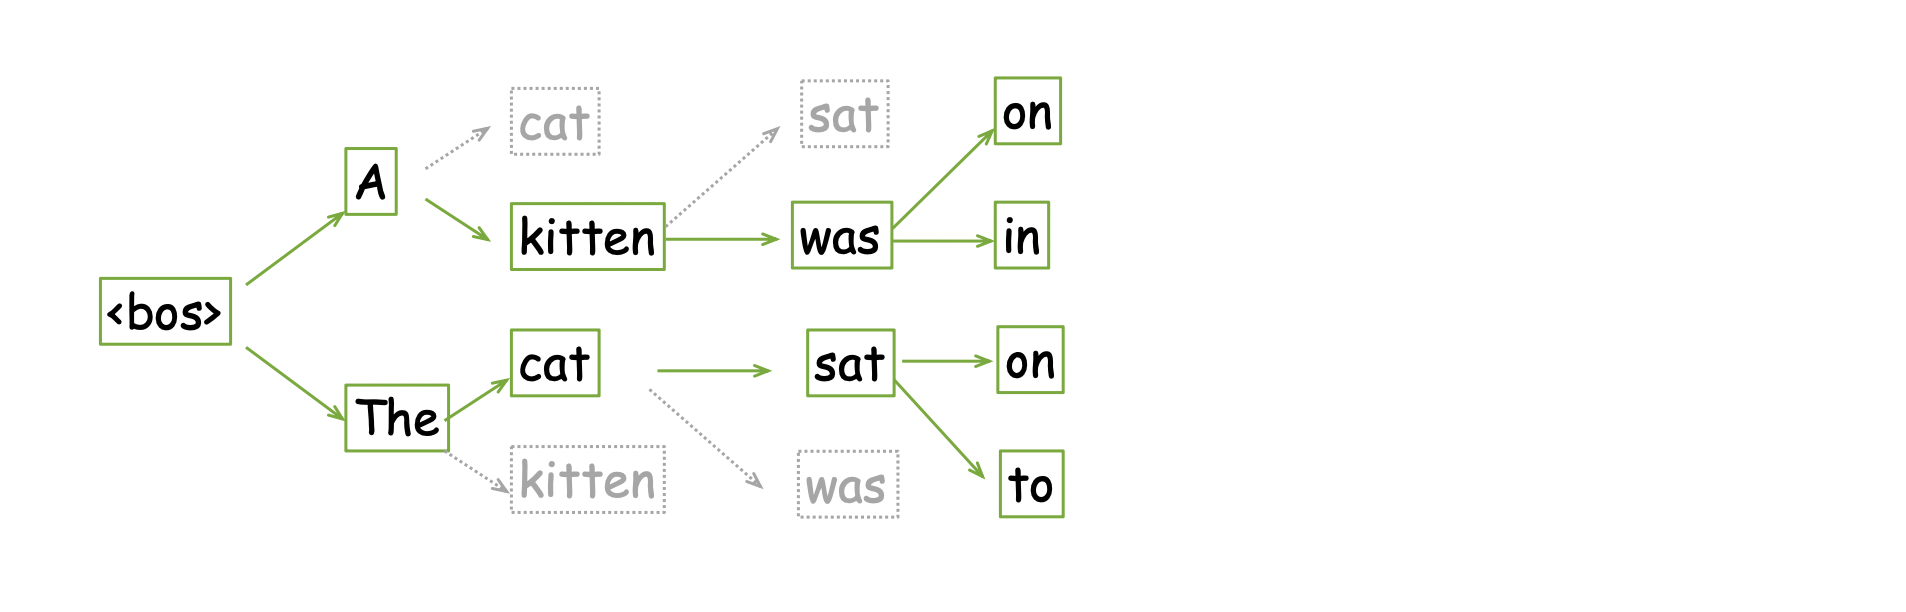
\includegraphics[width=.99\linewidth]{bs7.png}
	\end{center}
	\vfill
	\footnotesize  {\color{blue} \url{https://github.com/yandexdataschool/nlp_course/tree/2021/week04_seq2seq}} 
\end{frame} 

\begin{frame}{Beam Search}
	\begin{center}
		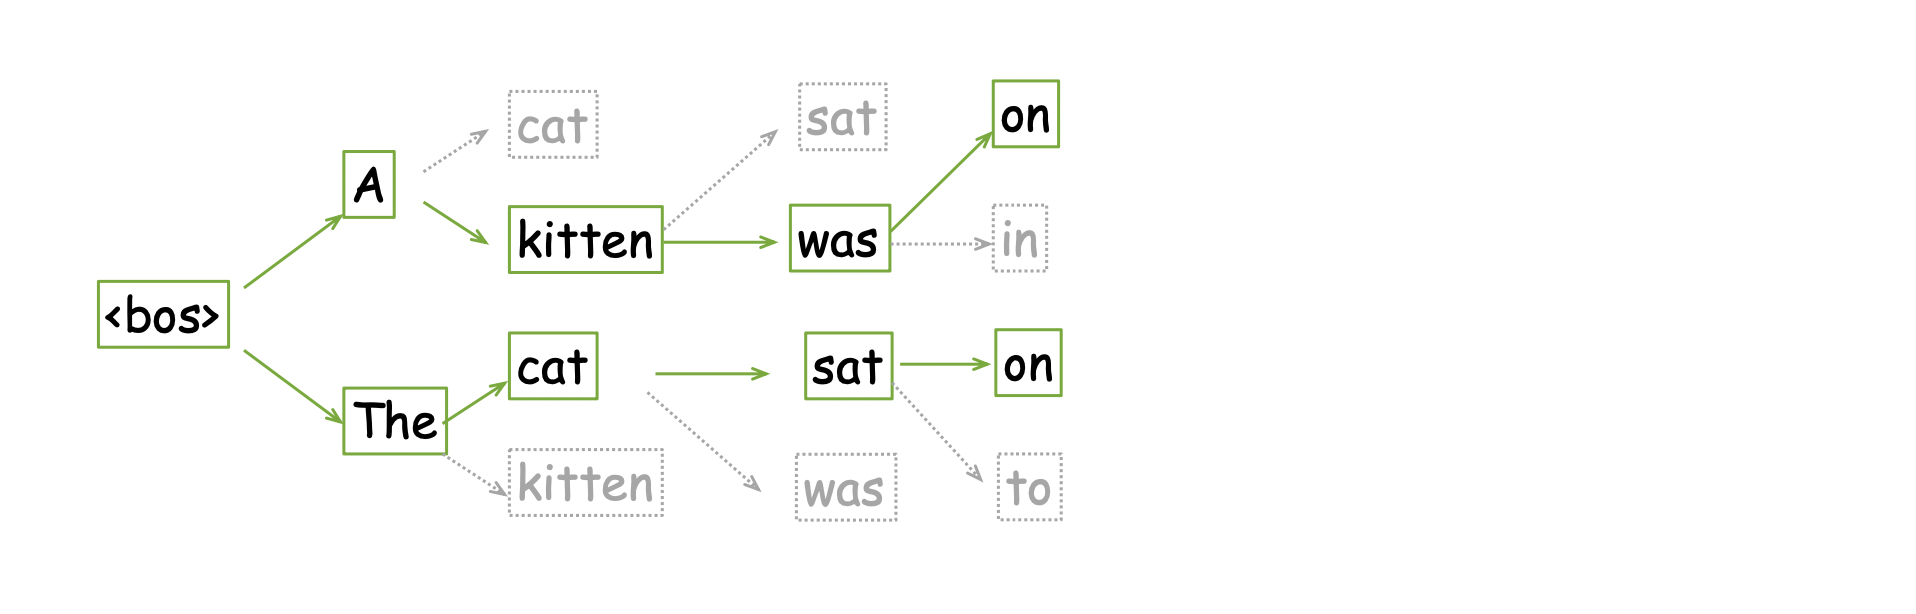
\includegraphics[width=.99\linewidth]{bs8.png}
	\end{center}
	\vfill
	\footnotesize  {\color{blue} \url{https://github.com/yandexdataschool/nlp_course/tree/2021/week04_seq2seq}} 
\end{frame} 

\begin{frame}{Beam Search}
	\begin{center}
		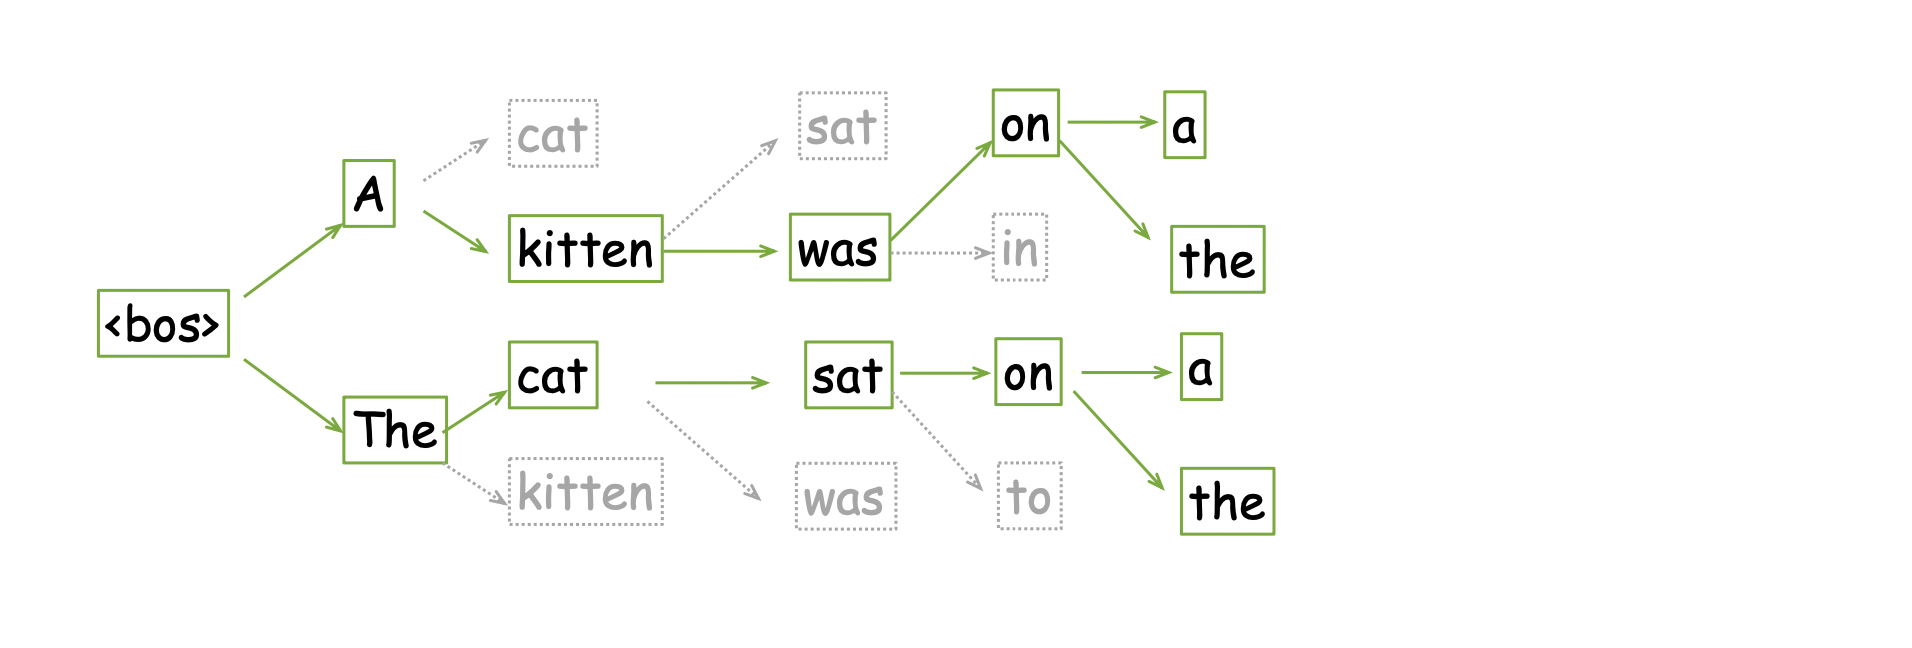
\includegraphics[width=.99\linewidth]{bs9.png}
	\end{center}
	\vfill
	\footnotesize  {\color{blue} \url{https://github.com/yandexdataschool/nlp_course/tree/2021/week04_seq2seq}} 
\end{frame} 

\begin{frame}{Beam Search}
	\begin{center}
		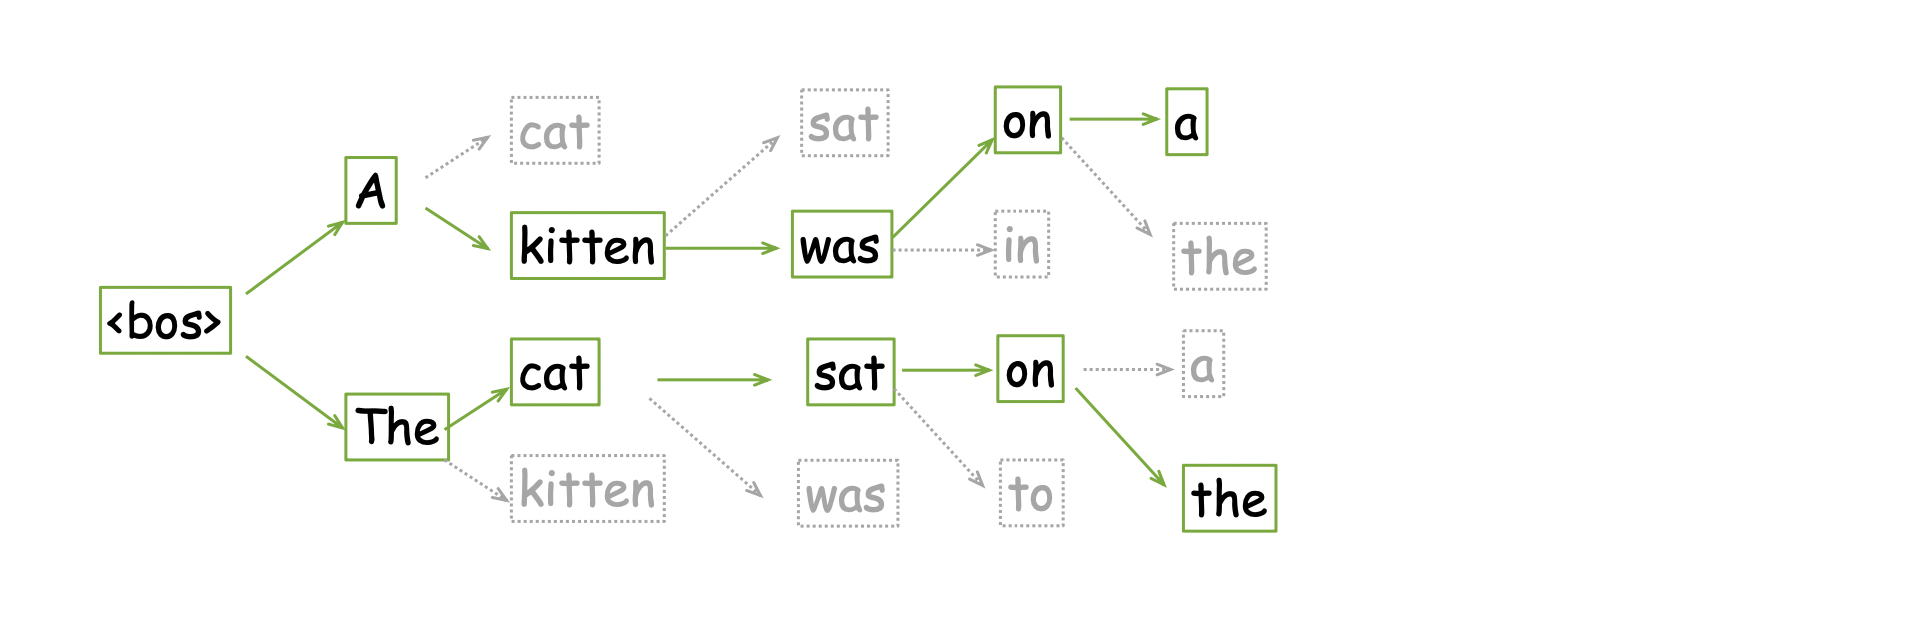
\includegraphics[width=.99\linewidth]{bs10.png}
	\end{center}
	\vfill
	\footnotesize  {\color{blue} \url{https://github.com/yandexdataschool/nlp_course/tree/2021/week04_seq2seq}} 
\end{frame} 

\begin{frame}{Beam Search}
	\begin{center}
		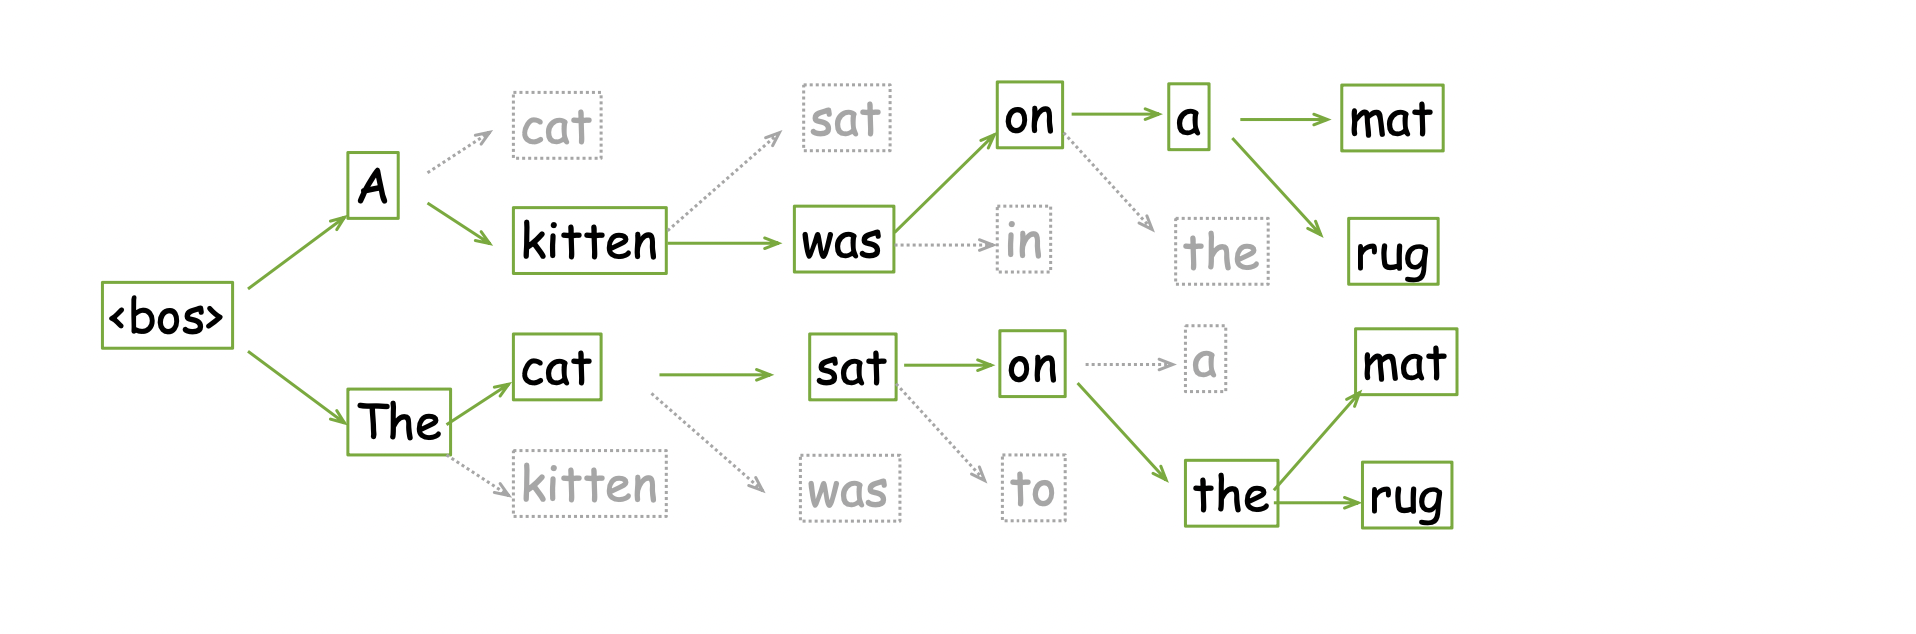
\includegraphics[width=.99\linewidth]{bs11.png}
	\end{center}
	\vfill
	\footnotesize  {\color{blue} \url{https://github.com/yandexdataschool/nlp_course/tree/2021/week04_seq2seq}} 
\end{frame} 

\begin{frame}{Beam Search}
	\begin{center}
		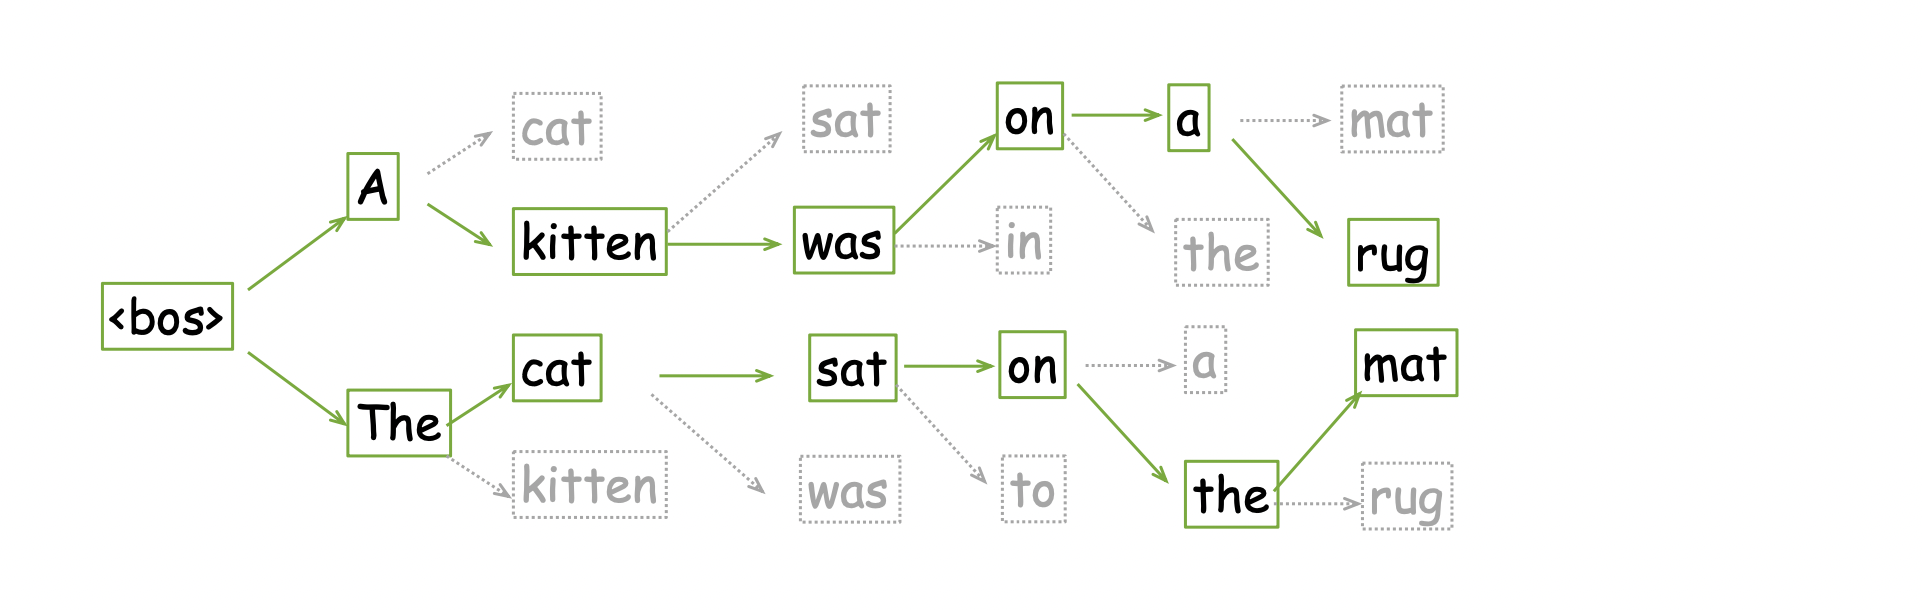
\includegraphics[width=.99\linewidth]{bs12.png}
	\end{center}
	\vfill
	\footnotesize  {\color{blue} \url{https://github.com/yandexdataschool/nlp_course/tree/2021/week04_seq2seq}} 
\end{frame} 

\begin{frame}{Beam Search}
	\begin{center}
		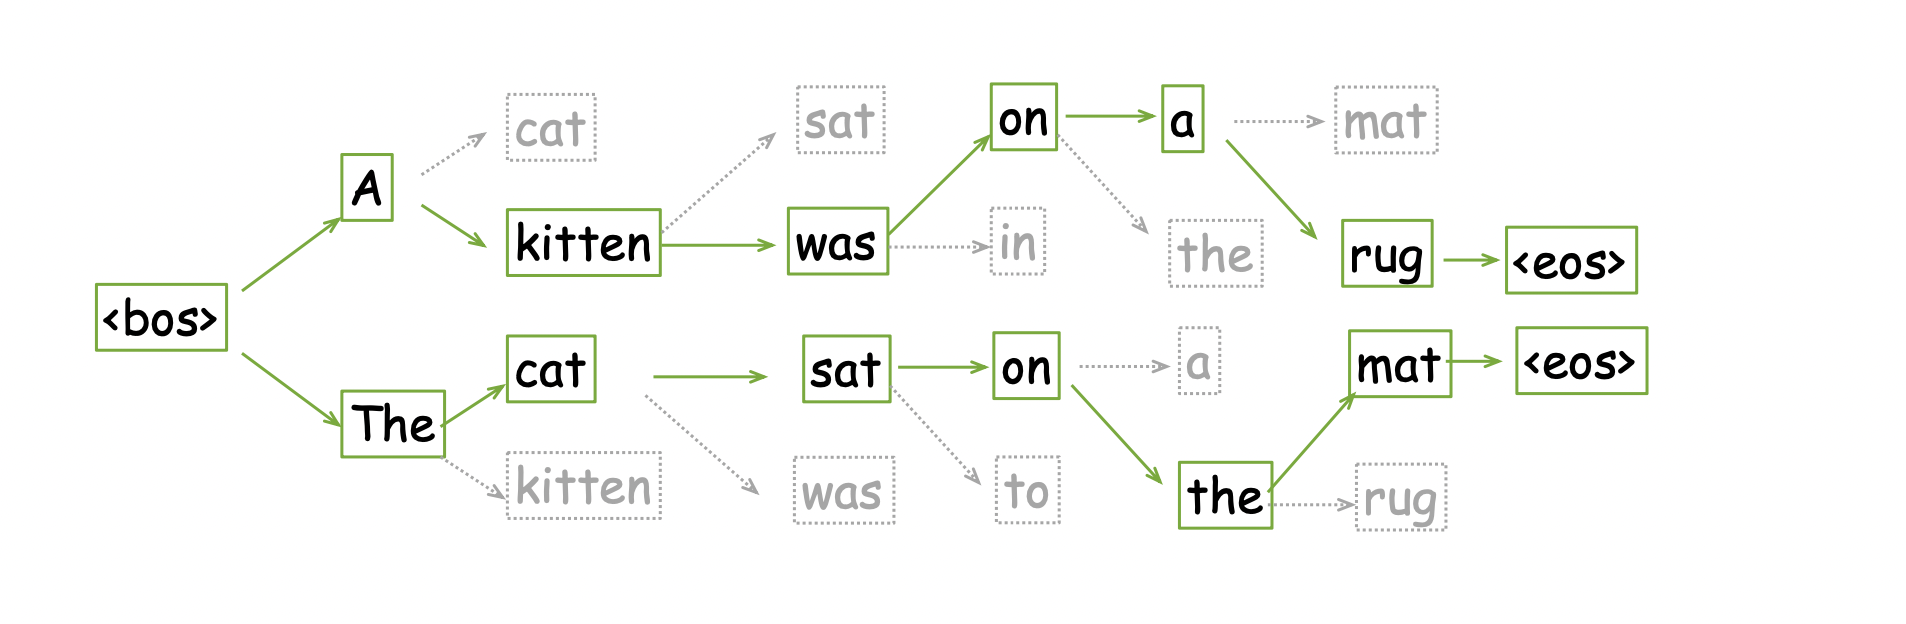
\includegraphics[width=.99\linewidth]{bs13.png}
	\end{center}
	\vfill
	\footnotesize  {\color{blue} \url{https://github.com/yandexdataschool/nlp_course/tree/2021/week04_seq2seq}} 
\end{frame} 

\begin{frame}{Beam Search}
	\begin{center}
		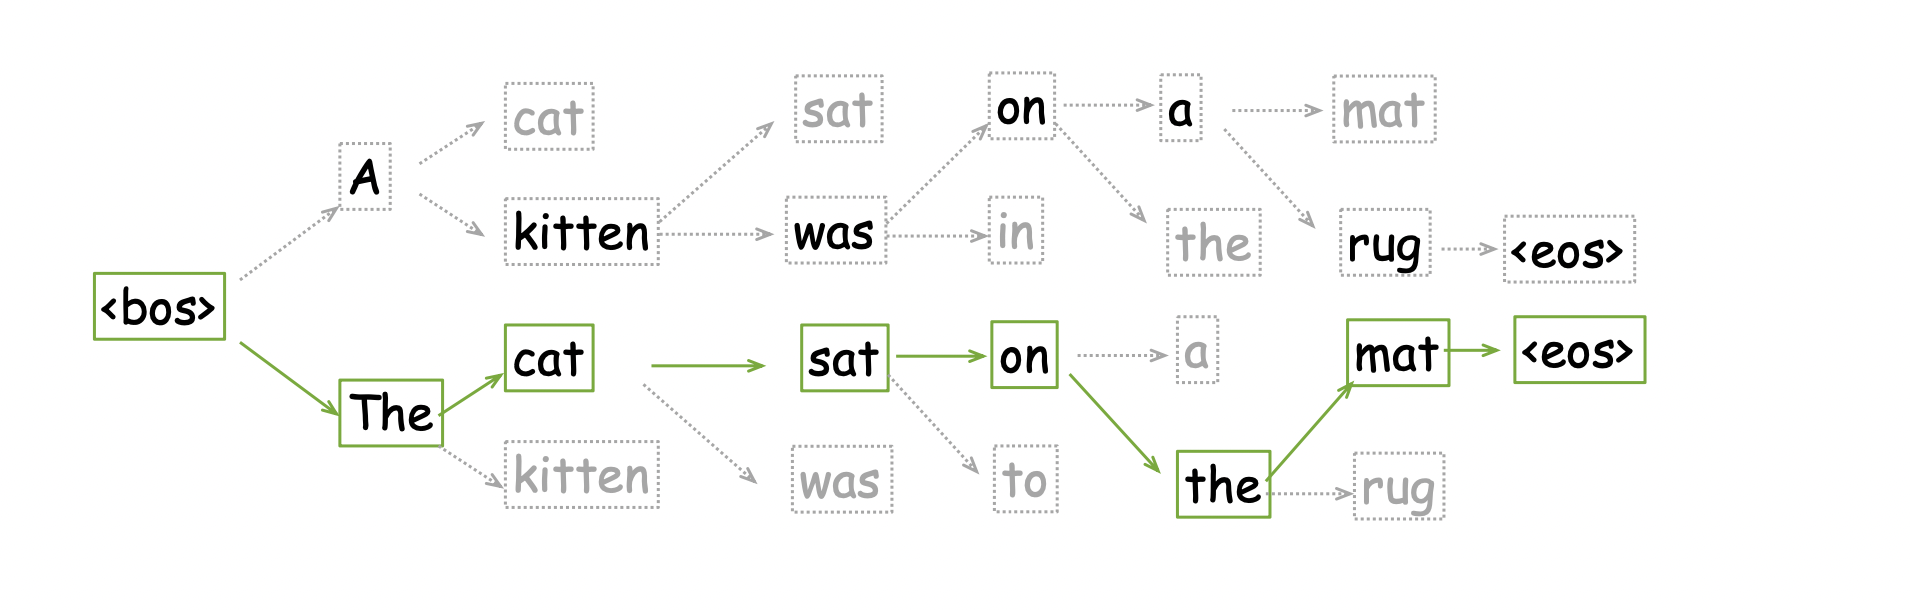
\includegraphics[width=.99\linewidth]{bs14.png}
	\end{center}
	\vfill
	\footnotesize  {\color{blue} \url{https://github.com/yandexdataschool/nlp_course/tree/2021/week04_seq2seq}} 
\end{frame} 


\begin{transitionframe}
	\begin{center}
		\Huge  Механизмы внимания
	\end{center}
\end{transitionframe}

\begin{frame}{В чём проблема простой RNN модели?}
	\begin{center}
		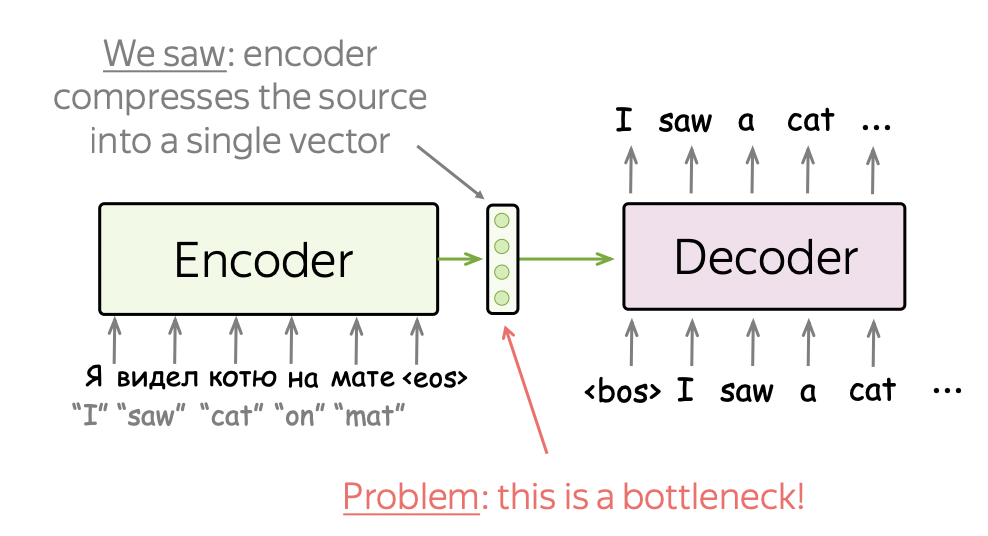
\includegraphics[width=.55\linewidth]{enc_problem.png}
	\end{center}
	\only<1>{
	\begin{wideitemize} 	
		\item  Сжать предложение в вектор сложно
		\item  Декодеру может понадобиться информация о разных частях предложения для его расшифровки
	\end{wideitemize} }
	\only<2>{
	\begin{wideitemize} 	
		\item  \alert{Attention:}  на разных шагах надо позволить модели фокусироваться на разных входных токенах
\end{wideitemize} }
	\vfill
	\footnotesize  {\color{blue} \url{https://github.com/yandexdataschool/nlp_course/tree/2021/week04_seq2seq}} 
\end{frame} 



\begin{frame}{Attention}
	\begin{center}
		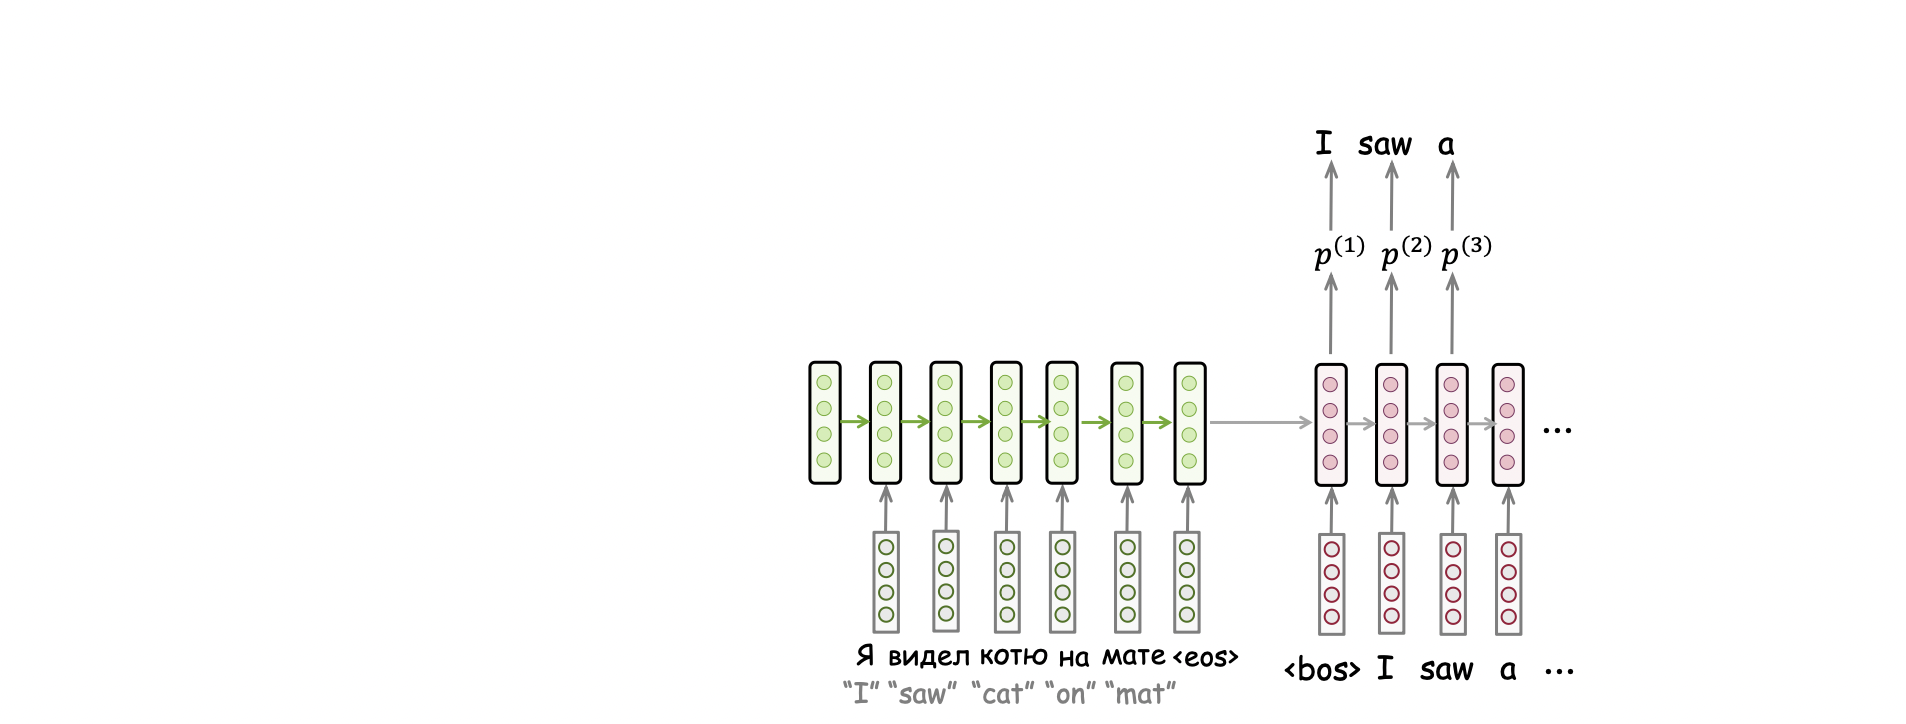
\includegraphics[width=.99\linewidth]{attention1.png}
	\end{center}
	\vfill
	\footnotesize  {\color{blue} \url{https://github.com/yandexdataschool/nlp_course/tree/2021/week04_seq2seq}} 
\end{frame} 

\begin{frame}{Attention}
	\begin{center}
		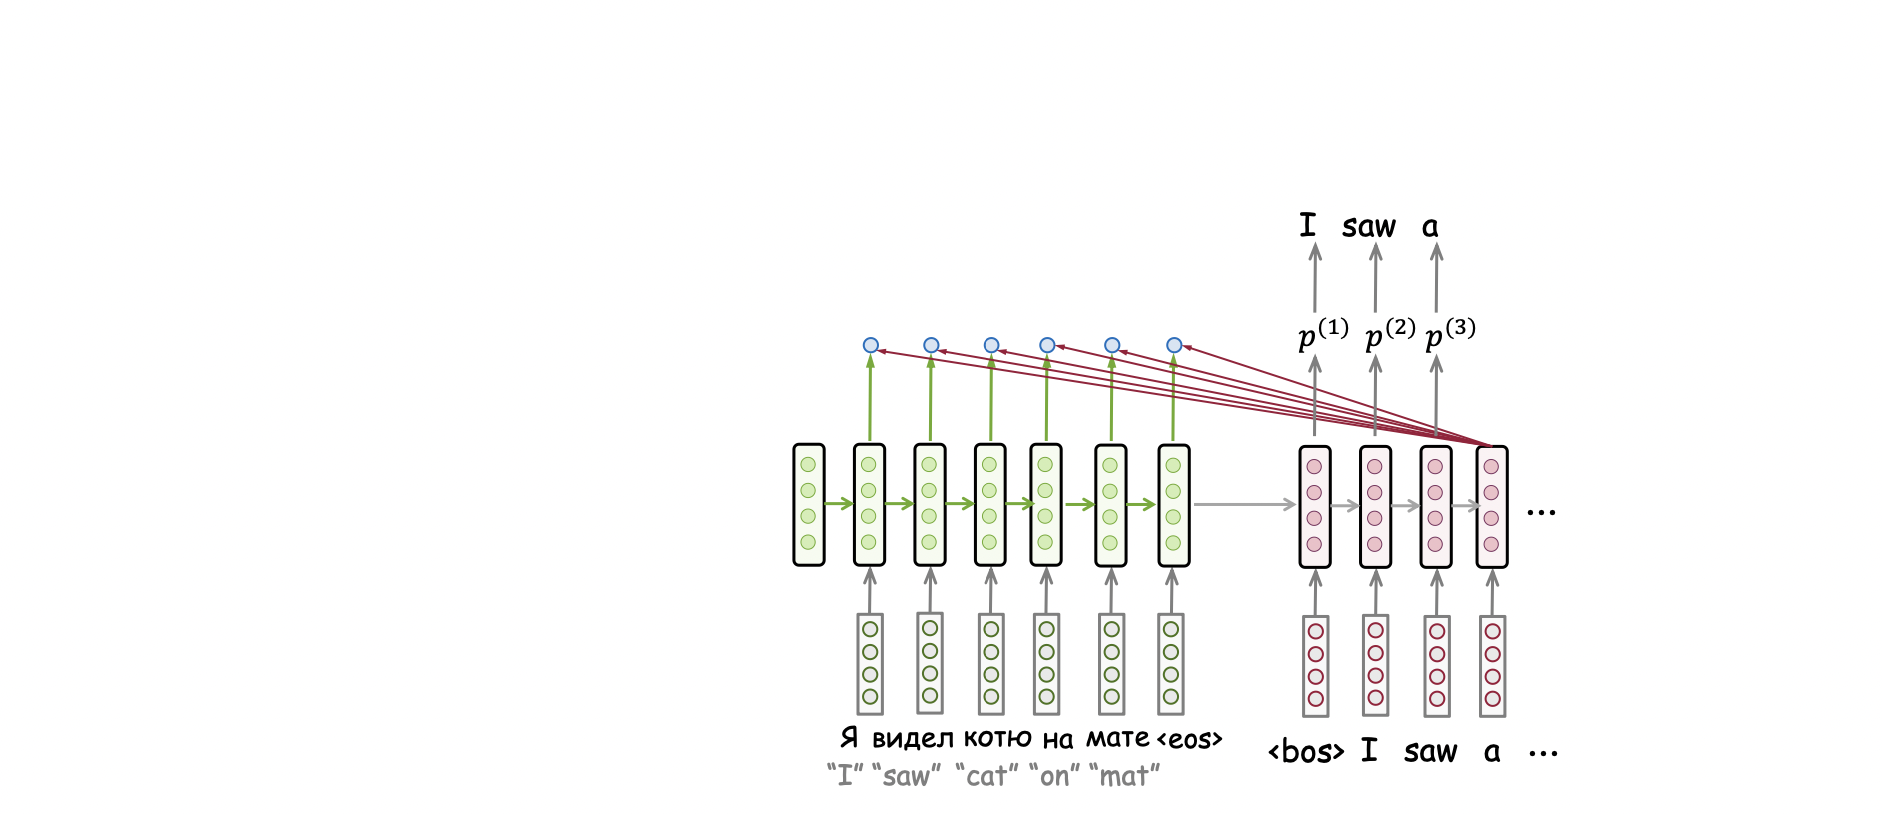
\includegraphics[width=.99\linewidth]{attention2.png}
	\end{center}
	\vfill
	\footnotesize  {\color{blue} \url{https://github.com/yandexdataschool/nlp_course/tree/2021/week04_seq2seq}} 
\end{frame} 

\begin{frame}{Attention}
	\begin{center}
		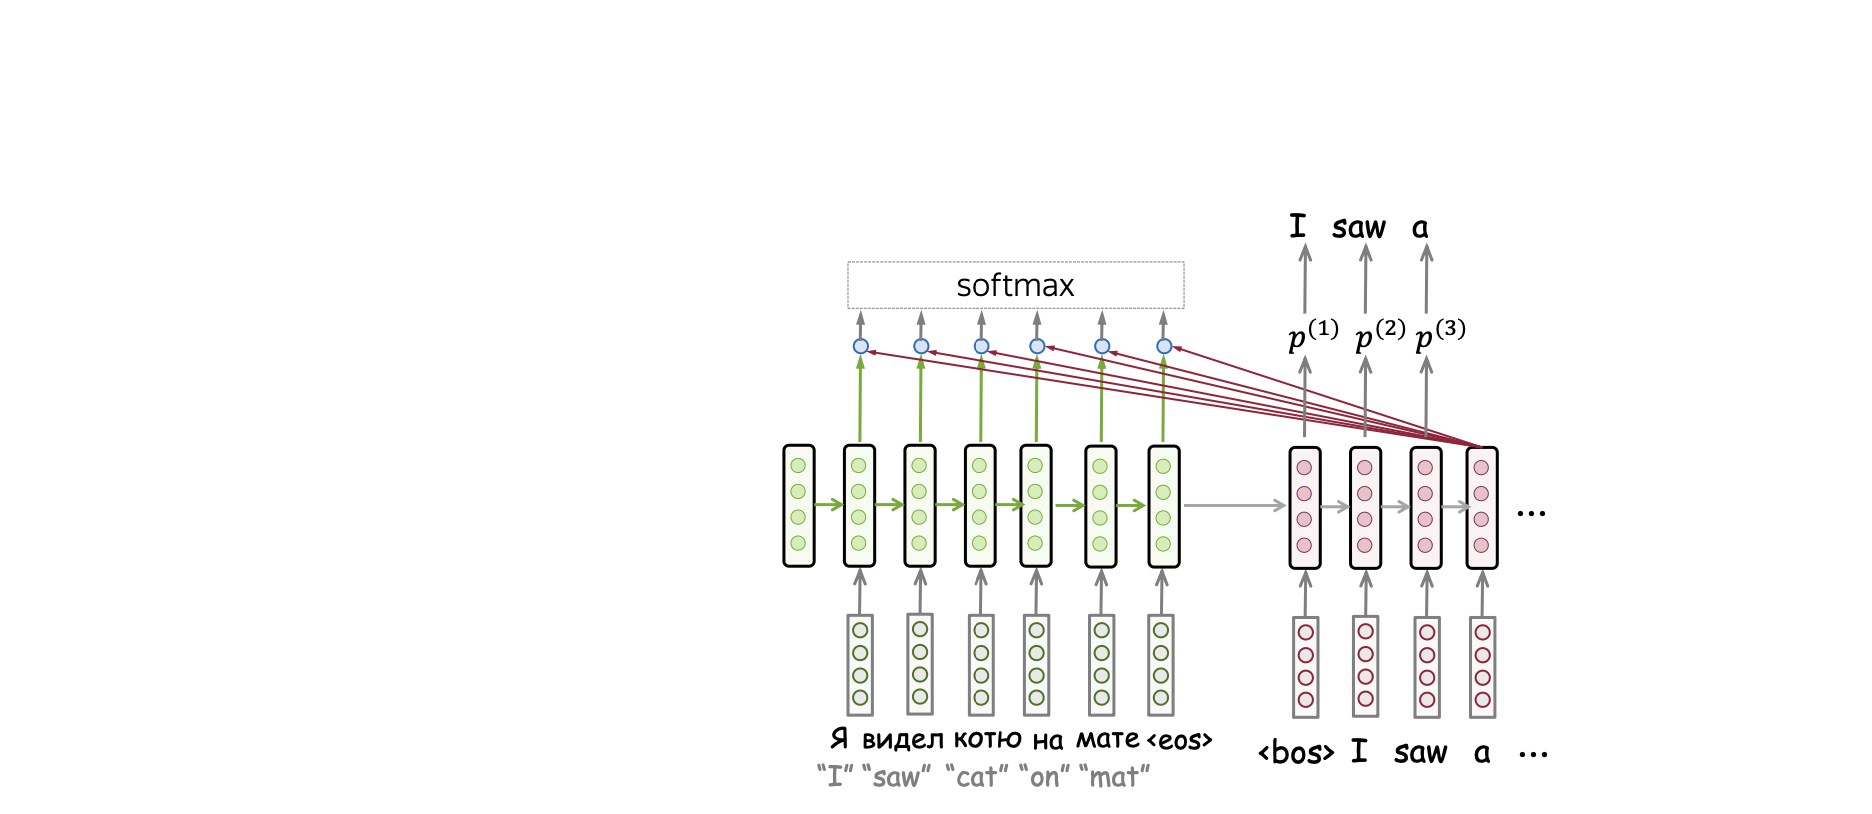
\includegraphics[width=.99\linewidth]{attention3.png}
	\end{center}
	\vfill
	\footnotesize  {\color{blue} \url{https://github.com/yandexdataschool/nlp_course/tree/2021/week04_seq2seq}} 
\end{frame} 

\begin{frame}{Attention}
	\begin{center}
		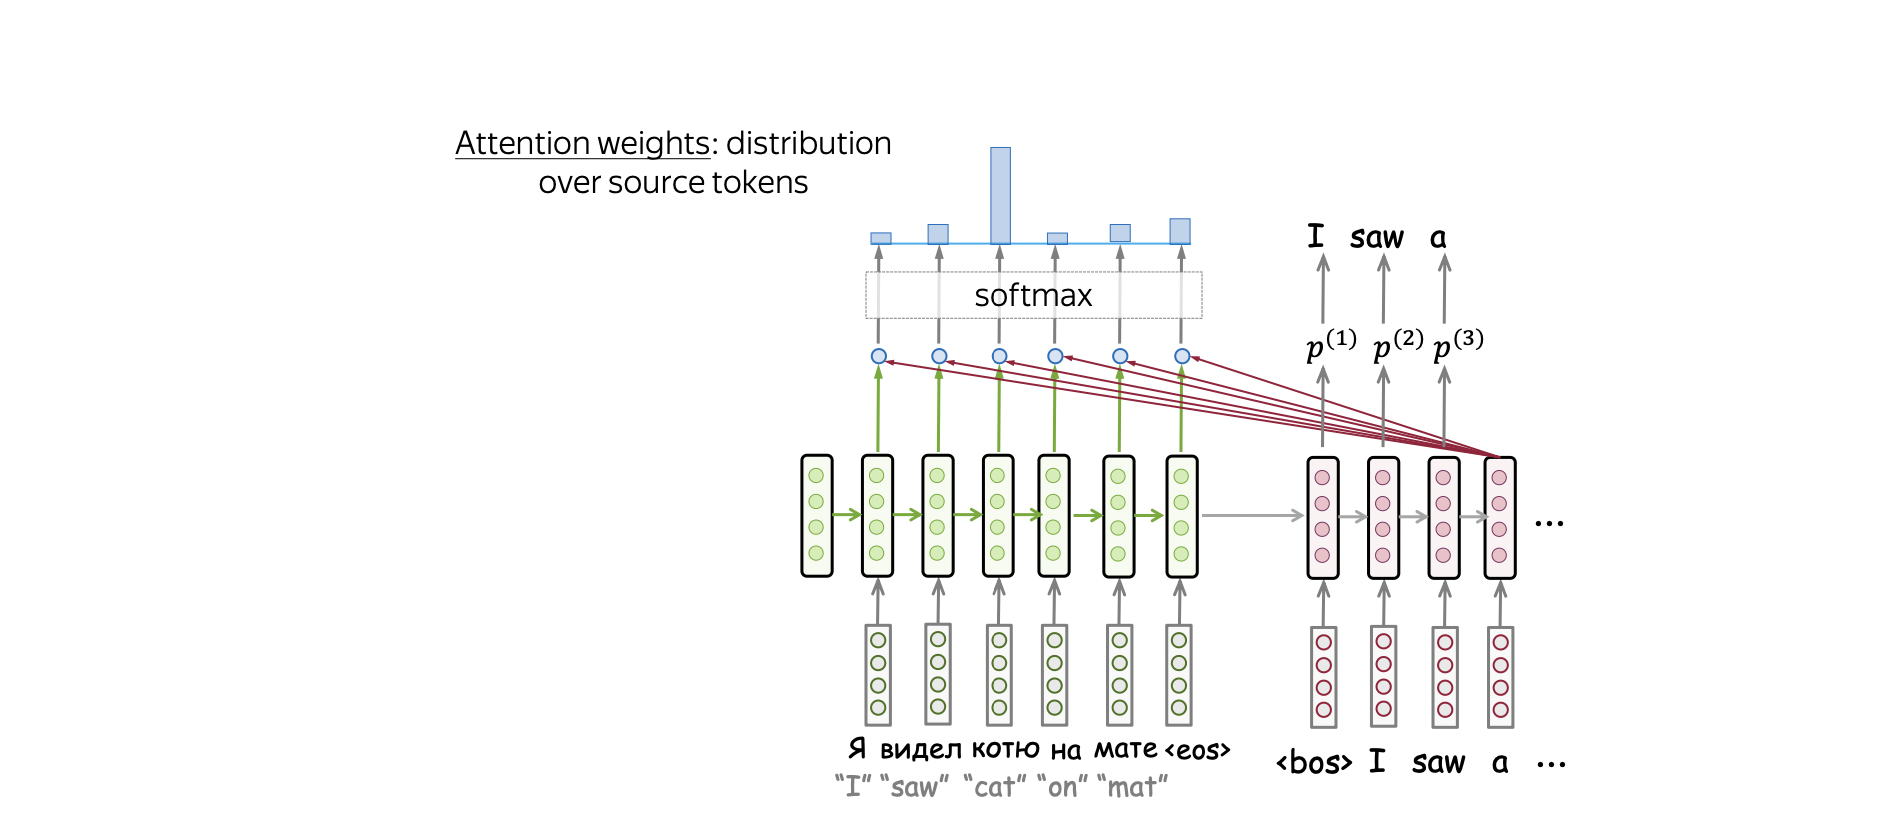
\includegraphics[width=.99\linewidth]{attention4.png}
	\end{center}
	\vfill
	\footnotesize  {\color{blue} \url{https://github.com/yandexdataschool/nlp_course/tree/2021/week04_seq2seq}} 
\end{frame} 

\begin{frame}{Attention}
	\begin{center}
		\includegraphics[width=.99\linewidth]{attention5.png}
	\end{center}
	\vfill
	\footnotesize  {\color{blue} \url{https://github.com/yandexdataschool/nlp_course/tree/2021/week04_seq2seq}} 
\end{frame} 

\begin{frame}{Attention}
	\begin{center}
		\includegraphics[width=.99\linewidth]{attention6.png}
	\end{center}
	\vfill
	\footnotesize  {\color{blue} \url{https://github.com/yandexdataschool/nlp_course/tree/2021/week04_seq2seq}} 
\end{frame} 

\begin{frame}{Attention}
	\begin{center}
		\includegraphics[width=.99\linewidth]{attention7.png}
	\end{center}
	\vfill
	\footnotesize  {\color{blue} \url{https://github.com/yandexdataschool/nlp_course/tree/2021/week04_seq2seq}} 
\end{frame} 



\begin{frame}{Computation Pipeline}
	\begin{center}
		\includegraphics[width=.9\linewidth]{pipe_1.png}
	\end{center}
	\vfill
	\footnotesize  {\color{blue} \url{https://github.com/yandexdataschool/nlp_course/tree/2021/week04_seq2seq}} 
\end{frame} 

\begin{frame}{Computation Pipeline}
	\begin{center}
		\includegraphics[width=.9\linewidth]{pipe_2.png}
	\end{center}
	\vfill
	\footnotesize  {\color{blue} \url{https://github.com/yandexdataschool/nlp_course/tree/2021/week04_seq2seq}} 
\end{frame} 

\begin{frame}{Computation Pipeline}
	\begin{center}
		\includegraphics[width=.9\linewidth]{pipe_3.png}
	\end{center}
	\vfill
	\footnotesize  {\color{blue} \url{https://github.com/yandexdataschool/nlp_course/tree/2021/week04_seq2seq}} 
\end{frame} 

\begin{frame}{Computation Pipeline}
	\begin{center}
		\includegraphics[width=.9\linewidth]{pipe_4.png}
	\end{center}
	\vfill
	\footnotesize  {\color{blue} \url{https://github.com/yandexdataschool/nlp_course/tree/2021/week04_seq2seq}} 
\end{frame} 




\begin{frame}{Внимание в декодере}
	\begin{center}
		\includegraphics[width=.9\linewidth]{attention_use_1.png}
	\end{center}
	\vfill
	\footnotesize  {\color{blue} \url{https://github.com/yandexdataschool/nlp_course/tree/2021/week04_seq2seq}} 
\end{frame} 

\begin{frame}{Внимание в декодере}
	\begin{center}
		\includegraphics[width=.9\linewidth]{attention_use_2.png}
	\end{center}
	\vfill
	\footnotesize  {\color{blue} \url{https://github.com/yandexdataschool/nlp_course/tree/2021/week04_seq2seq}} 
\end{frame} 

\begin{frame}{Внимание в декодере}
	\begin{center}
		\includegraphics[width=.9\linewidth]{attention_use_3.png}
	\end{center}
	\vfill
	\footnotesize  {\color{blue} \url{https://github.com/yandexdataschool/nlp_course/tree/2021/week04_seq2seq}} 
\end{frame} 

\begin{frame}{Внимание в декодере}
	\begin{center}
		\includegraphics[width=.9\linewidth]{attention_use_4.png}
	\end{center}
	\vfill
	\footnotesize  {\color{blue} \url{https://github.com/yandexdataschool/nlp_course/tree/2021/week04_seq2seq}} 
\end{frame} 

\begin{frame}{Внимание в декодере}
	\begin{center}
		\includegraphics[width=.9\linewidth]{attention_use_5.png}
	\end{center}
	\vfill
	\footnotesize  {\color{blue} \url{https://github.com/yandexdataschool/nlp_course/tree/2021/week04_seq2seq}} 
\end{frame} 

\begin{frame}{Внимание в декодере}
	\begin{center}
		\includegraphics[width=.9\linewidth]{attention_use_6.png}
	\end{center}
	\vfill
	\footnotesize  {\color{blue} \url{https://github.com/yandexdataschool/nlp_course/tree/2021/week04_seq2seq}} 
\end{frame} 

\begin{frame}{Внимание в декодере}
	\begin{center}
		\includegraphics[width=.9\linewidth]{attention_use_7.png}
	\end{center}
	\vfill
	\footnotesize  {\color{blue} \url{https://github.com/yandexdataschool/nlp_course/tree/2021/week04_seq2seq}} 
\end{frame} 

\begin{frame}{Внимание в декодере}
	\begin{center}
		\includegraphics[width=.9\linewidth]{attention_use_8.png}
	\end{center}
	\vfill
	\footnotesize  {\color{blue} \url{https://github.com/yandexdataschool/nlp_course/tree/2021/week04_seq2seq}} 
\end{frame} 




\begin{frame}{Attention Score Functions}
	\begin{center}
		\includegraphics[width=.9\linewidth]{att_sc_f_1.png}
	\end{center}
	\vfill
	\footnotesize  {\color{blue} \url{https://github.com/yandexdataschool/nlp_course/tree/2021/week04_seq2seq}} 
\end{frame} 

\begin{frame}{Attention Score Functions}
	\begin{center}
		\includegraphics[width=.9\linewidth]{att_sc_f_2.png}
	\end{center}
	\vfill
	\footnotesize  {\color{blue} \url{https://github.com/yandexdataschool/nlp_course/tree/2021/week04_seq2seq}} 
\end{frame} 

\begin{frame}{Attention Score Functions}
	\begin{center}
		\includegraphics[width=.9\linewidth]{att_sc_f_3.png}
	\end{center}
	\vfill
	\footnotesize  {\color{blue} \url{https://github.com/yandexdataschool/nlp_course/tree/2021/week04_seq2seq}} 
\end{frame} 

\begin{frame}{Attention Score Functions}
	\begin{center}
		\includegraphics[width=.9\linewidth]{att_sc_f_4.png}
	\end{center}
	\vfill
	\footnotesize  {\color{blue} \url{https://github.com/yandexdataschool/nlp_course/tree/2021/week04_seq2seq}} 
\end{frame} 




\begin{frame}{Bahdanau Model (the original attention model)}
	\begin{center}
		\includegraphics[width=.9\linewidth]{bogdanof_model.png}
	\end{center}
	\vfill
	\footnotesize  {\color{blue} \url{https://github.com/yandexdataschool/nlp_course/tree/2021/week04_seq2seq}} 
\end{frame} 

\begin{frame}{Luong Model}
	\begin{center}
		\includegraphics[width=.9\linewidth]{luong_model.png}
	\end{center}
	\vfill
	\footnotesize  {\color{blue} \url{https://github.com/yandexdataschool/nlp_course/tree/2021/week04_seq2seq}} 
\end{frame} 



\begin{frame}{Attention}
	\begin{center}
		\includegraphics[width=.9\linewidth]{attention.png}
	\end{center}
	\vfill
	\footnotesize  {\color{blue} \url{https://arxiv.org/pdf/1409.0473.pdf}} 
\end{frame} 


\end{document}



